\documentclass[a4paper, 12pt, openany]{report} %chose the paper size and font size. Openany ensures that all all chapters and similar may begin at any page, not only odd pages. For the introductory pages and appendices we want openany, but for chapter pages in the main content we want chapters to begin only on odd pages (right hand side). The book class ensures that the margins are automatically adjusted such that left hand pages are slightly moved to the left and vice versa at the right, which makes the thesis very readable and good-looking when printed in bound book format.
\usepackage{comment}
\usepackage{enumitem}
\setlistdepth{10}
\usepackage[utf8]{inputenc} %to manage special characters
\usepackage[T1]{fontenc} %to manage special characters
\usepackage[Bjarne]{fncychap} %fancy chapter style (much more available, like Sonny or Lenny, etc.)
\usepackage{fancyhdr} %to customize the headers
\usepackage[lmargin=1.5in, rmargin=1in, tmargin=1in, bmargin=1in]{geometry} %sets the margins for the pages
\setcounter{tocdepth}{2} %table of contents number depth for subsections (2 = x.x.x)
\setcounter{secnumdepth}{4} %numbering depth for headers for subsections in the text(4 = x.x.x.x)
\usepackage{url} %to include URLs
\usepackage{pdfpages}
\usepackage{listings} %include this if you want to include code in the thesis
\usepackage{amsmath,amssymb} %mathematical package
\usepackage{siunitx} %includes SI-units
\usepackage[bf]{caption} %makes float captions bold
\usepackage{array, booktabs} %to make better tables
\usepackage{graphicx} %to include graphics
\usepackage{float} %to include floats
\usepackage[export]{adjustbox} %to adjust floats
\usepackage{subfig} %to include subfigures
\usepackage{chngcntr} %will make it possible to change the counter for tables, figures, etc. such as below
\counterwithin{figure}{section} %change counter for figures within sections (also possible to choose for each chapter
\counterwithin{table}{section} %change counter for tables within sections
\usepackage{color, xcolor} %edit e.g. text colors
\usepackage{hyperref}
\usepackage{graphicx} % for including graphics
\usepackage{pgffor}   % for the \foreach loop
\usepackage{etoolbox} % for \csedef

\usepackage{fancyvrb}
\DefineVerbatimEnvironment{Verbatim}{Verbatim}{fontsize=\footnotesize}


\usepackage{ragged2e}
\pretolerance=5000
\tolerance=5000
\emergencystretch=50pt

\usepackage{tikz} % self added
\usetikzlibrary{positioning} % self addded


\usepackage[backend = biber,
            style = numeric,
            date = long,     % Long: 24th Mar. 1997 | Short: 24/03/1997
            sorting = none,
            maxcitenames = 3,   % max names to include before et. al.
            ]{biblatex} %customize the look of your citations and bibliography
\addbibresource{bibliography.bib} %declare the bibliography resource
\usepackage{comment} %to be able to comment out sections in the .tex files
\usepackage{afterpage} %to customize page commands such as below
\newcommand\myemptypage{
    \null
    \thispagestyle{empty}
    \addtocounter{page}{-1}
    \newpage
    } %sets the new page command to insert an empty page without adding to the page counter or having a page number




\begin{document}
%%%%%%%%%%%%%%%%%%%%%%%%%%%%%%%%%%%%%%%%%%%%%%%%%%%%%%%%
%\begin{comment}
% The title page:
% For NTNU students this page will be generated automatically when submitting your paper, and should not be included in the final file from Latex. Delete or comment out the title page setup. The final report should then start with the first page being the abstract. I have included a title page here so it is possible to see what it may look like, and for those who do not get an automatically generated title page. Of course, you must change your case's names and titles, etc...

% The title page should be an odd page (right hand side)

%\begin{titlepage}
%\newgeometry{left=1.6in, right=2in}
%\vspace*{1.5cm}

%\noindent  \textcolor{gray}{\large Erlend Withammer-Ekerhovd} \\
%\vspace{1cm}

%\noindent \textbf{\Large Classifying States of Attention and Mind Wandering from EEG signals} \\
%\vspace{0.5cm}

%\noindent {\large : A Tool for Assessing the Efficacy and Progression of Contemplative Practices} \\



%\vspace{7cm}
%\noindent Master's thesis in Cybernetics and Robotics \\
%Supervisor: Marta Molinas \\
%Co-supervisors: Andres Soler, Amandeep Cheema \\
%June 2024 \\

%\vspace{0.2cm}
%\noindent Norwegian University of Science and Technology \\
%Faculty of Information Technology and Electrical Engineering \\
%Department of Engineering Cybernetics \\

%\begin{figure}[h]
%    
\includegraphics[width=0.28\textwidth]{Figures/ntnu_basic.png}
%\end{figure}
%\end{titlepage}
%\restoregeometry
%\myemptypage %empty page such that the abstract starts at the first right-hand side after the title page
%\end{comment}
%%%%%%%%%%%%%%%%%%%%%%%%%%%%%%%%%%%%%%%%%%%%%%%%%%%%%%%%

% The pre-chapters
\chapter*{Abstract} %pre-chapters should not be numbered, hence the "*"
\pagenumbering{roman} %introductory pages should be roman
\setcounter{page}{1}
\addcontentsline{toc}{chapter}{\protect\numberline{}Abstract} %add the chapter to the table of contents, this is not automatically added when creating unnumbered chapters (*). Add it in a chapter style, and keep all chapters on the same number line indent regardless of number or not on the chapter

This thesis explores contemplative practices and cognitive neuroscience through machine learning applied to EEG data, laying the groundwork for developing a methodological framework assessing mind wandering. With a growing body of research underscoring the benefits of practices such as meditation on mental health, there is a critical need for objective tools to measure their impact effectively.

Leveraging a dataset that includes EEG recordings from tasks designed to induce mind wandering, this work focuses on building and refining a Convolutional Neural Network (CNN) based on the EEGNeX architecture. The primary goal is to classify states of attention and mind wandering, thereby providing a tool to assess the efficacy and progression of contemplative practices. This classification aids in understanding how these practices influence cognitive processes and mental states, which can be particularly useful for tailoring individual therapeutic approaches in clinical settings.

In developing this CNN, various data balancing techniques were applied to address class imbalances, and noise reduction strategies were employed to enhance the quality of EEG signals. The model was trained and validated using rigorous cross-validation techniques to ensure its robustness and generalizability across different individuals and contemplative states using two different mind-wandering-inducing tasks.

The findings from this thesis could contribute to contemplative neuroscience by offering insights into methods for classifying neural mechanisms underlying mind wandering. This work provides a foundation for future research and the development of objective measures of progress in contemplative practices for possible improvements in mental health.

Ultimately, this thesis underscores the potential of combining traditional contemplative practices with modern neuroscience and machine learning techniques, paving the way for innovative approaches to enhancing well-being and treating mental health conditions.

\newpage
\chapter*{Sammendrag}

Denne Masteroppgaven utforsker kontemplative praksiser gjennom bruk av maskinlæring på EEG-data, med mål om å utvikle et metodisk rammeverk for å vurdere tankevandring (Mind Wandering) og meditative tilstander. Med en økende mengde forskning på feltet som understreker fordelene med øvelser som meditasjon og yoga på mental helse, er det et stort behov for objektive verktøy for måling av deres innvirkning på kropp og sinn.

Ved å utnytte et datasett som inkluderer EEG-opptak fra oppgaver designet for å forårsake tankevandring, fokuserer denne masteroppgaven på å lage og finjustere et konvolusjonsnettverk (CNN) basert på EEGNeX-arkitekturen. Hovedmålet er å klassifisere tilstander av oppmerksomhet og tankevandring, noe som gir et verktøy for å vurdere effektiviteten av, og individers fremgangen i, kontemplative praksiser. Denne klassifiseringen bidrar til å forstå hvordan disse praksisene påvirker kognitive prosesser og mentale tilstander, noe som kan være spesielt nyttig for å skreddersy individuelle terapeutiske tilnærminger.

I prosessen med å utvikle denne CNN modellen ble ulike teknikker for datautjevning anvendt for å takle klasseubalanser, og støyreduksjonsstrategier ble benyttet for å forbedre kvaliteten på EEG-signalene. Modellen ble trent og validert ved hjelp av kryssvalideringsteknikker for å sikre dens robusthet og generaliserbarhet på tvers av ulike individer og kontemplative tilstander ved bruk av to ulike tankevandringsfremmende øvelser.

Funnene fra denne avhandlingen kan bidra  til feltene kontemplativ nevrovitenskap og mental helse, og tilby nye innsikter i de nevrale mekanismene som ligger til grunn for meditasjon og tankevandring. Dette arbeidet gir et grunnlag for videre forskning på området, og har potensial til å veilede utviklingen av målrettede anvendelser av kontemplative praksiser for mental helse og kognitiv forbedring.

Til slutt påpeker denne avhandlingen potensialet for å kombinere tradisjonelle kontemplative praksiser med moderne nevrovitenskap og maskinlæringsteknikker, og baner vei for innovative tilnærminger til å forbedre velvære og behandle psykiske helseproblemer.





 %insert the chapter text from the files

\chapter*{Preface}
\addcontentsline{toc}{chapter}{\protect\numberline{}Preface} 
This thesis is the result of my academic and personal journey into the fields of contemplative practices and cognitive neuroscience. Ever since I started meditating, I've been interested in the topics. My personal experience with meditation has improved my focus and emotional regulation, which sparked my curiosity about the scientific basis of these practices. I believed that there might have been a difference between the popular claims about meditation and the scientific research. I wanted to explore this gap in hopes of grounding my practice in empirical evidence and strengthening my commitment to it.
\newline
Conducting this research has not been without its challenges. The gap in practical alignment between my master's thesis and the preceding project thesis presented a steep learning curve, as it felt like starting from scratch. I found myself navigating the complexities of high-performance computing interfaces and delving into the intricacies of CNNs with limited prior experience. Moreover, working with EEG data introduced a unique set of challenges, from understanding its specific requirements to adapting methodologies that would faithfully capture and interpret the nuances of such data.
\newline
Throughout this process, constructing a scalable and robust code base emerged as a crucial lesson. The flexibility and efficiency of handling large datasets, especially when not initially prepared for the complex analyses planned, became apparent as a foundational skill. Furthermore, the decision to use a dataset not collected by our team introduced additional hurdles in data interpretation and required adaptations to fit our analytical framework.
\newline
Collaboration played a pivotal role in overcoming many of these obstacles. I was fortunate to connect with the lead author of our dataset, Christina Yi Jin, who provided invaluable assistance by clarifying data specifics and supplying missing components essential for our analyses. While this interaction did not directly influence our research outcomes, it enabled us to use the dataset effectively, highlighting the importance of collaboration in scientific endeavors.
\newline
I envision this thesis as a stepping stone toward developing more refined tools for measuring and understanding mind-wandering and meditative states. These tools have immense potential to advance scientific knowledge and provide practical benefits in meditation training. I aspire for future researchers to build upon this work, expanding the dataset, enhancing methodological rigor, and perhaps integrating these tools into systems that offer real-time, personalized guidance for meditators.
\newline
I want to thank my supervisor, Marta Molinas, whose guidance was invaluable throughout this journey. Her expertise and insightful feedback were crucial in shaping the direction and execution of this research. I am profoundly grateful to my girlfriend, Isabella Starrfield, for her support and understanding throughout the ups and downs of this project. Her encouragement has been a constant source of motivation, and without it, this thesis would not be completed on time.
\newline
I am also incredibly thankful to my parents, whose love and support have been foundational throughout my life. Their encouragement and belief in my abilities have always been precious to me.
This thesis is dedicated to all who find meditation a path to greater clarity and peace and the scientific community that seeks to understand how such simple practices can effect profound changes in our minds and bodies. I hope this work contributes meaningfully to both realms, bridging the gap between anecdotal benefits and scientific validation.
\newline
With gratitude,\newline
Erlend Withammer-Ekerhovd

\tableofcontents
\addcontentsline{toc}{chapter}{\protect\numberline{}Contents}

%add to table of contents list of figures and tables, and insert list of figures and tables
\addcontentsline{toc}{chapter}{\protect\numberline{}\listfigurename}
\listoffigures
\addcontentsline{toc}{chapter}{\protect\numberline{}\listtablename}
\listoftables


\chapter*{Abbreviations}
\addcontentsline{toc}{chapter}{\protect\numberline{}Abbreviations}
% Put in your abbreviations here

List of all abbreviations in alphabetic order:

\begin{itemize}
\item \textbf{BW} Breath Work
\item \textbf{CNN} Convolutional Neural Network
\item \textbf{DS} Distracted
\item \textbf{ECG} Electrocardiogram
\item \textbf{EEG} Electroencephalogram
\item \textbf{ERP} Event-Related Potential
\item \textbf{HPC} High-Performance Computing
\item \textbf{HRV} Heart Rate Variability
\begin{itemize}
            \item \textbf{HF-HRV} High-Frequency HRV
            \item \textbf{LF-HRV} Low-Frequency HRV
\end{itemize}
\item \textbf{IDUN} NTNU's HPC System
\item \textbf{IMF} Intrinsic Mode Functions
\item \textbf{LNPO} Leave N Participants Out
\item \textbf{LOPO} Leave One Participant Out
\item \textbf{MEMD} Multidimensional Empirical Mode Decomposition
\item \textbf{ML} Machine Learning
\item \textbf{MM} Mindfulness Meditation
\item \textbf{MW} Mind Wandering
\item \textbf{NN} Neural Network
\item \textbf{NTNU} Norwegian University of Science and Technology
\item \textbf{OT} On Task
\item \textbf{SART} Sustained Attention to Respons Task
\item \textbf{UC} Unclear
\item \textbf{VS} Visual Search

\end{itemize}
\newpage
\myemptypage
% Add an empty non-counted page by the command below to get the first chapter on the left-hand side if needed (check your page number so that the first chapter is on an odd page)


%%%%%%%%%%%%%%%%%%%%%%%%%%%%%%%%%%%%%%%%%%%%%%%%%%%%%%%%
%Customize the layout of the main content of your thesis

\pagestyle{fancy} %set customized page style for header
\fancyhf{} %clear header and footer fields
\renewcommand{\headrulewidth}{0pt} %set to no rule
\fancyhead[LE, RO]{\thepage} %set the page number at left for even, right for odd pages
\fancyhead[RE, LO]{\leftmark} %set the chapter name at right for even, left for odd pages
% Is it possible to design the header with the chapter as you wish, e.q. only the chapter or only the name, all lowercase instead, etc?
% You could also design the footer if you wish, for example:
%\fancyfoot[LE, RO]{\thepage}
\setlength{\headheight}{14.49998pt} %set the header height


%%%%%%%%%%%%%%%%%%%%%%%%%%%%%%%%%%%%%%%%%%%%%%%%%%%%%%%%
%main content 

\pagenumbering{arabic}
\chapter{Introduction}

% The subsections written are only suggestions to display how sections and subsections may look for your thesis

\section{Motivation}
Contemplative practices, traditional methods of disciplined mental and physical training, enhance self-awareness, inquiry, and regulation \cite{Davidson2017VarietiesOC}. They promote sustained, non-judgmental attention and introspection, providing a peaceful refuge in daily life. This centered tranquility aids in exploring life's deeper meanings and values. Among these practices are meditation, yoga, breathwork, prayer, and mindful walking \cite{Bruce2018ContemplativePP}. \footnote{The motivation for this master thesis is based on the motivation from the preceding project thesis on the same topic provided in \autoref{Appendix C}}

Traditionally maintained by spiritual figures like priests and yogis, these practices have recently gained broader popularity \cite{Brandmeyer2021MeditationAT}. Recent studies have found that 14.3\% of U.S. adults practice yoga and meditation, with about 17.5\% engaging in some form of mind-body therapy \cite{14USA}\cite{33USA}. During the COVID-19 pandemic's initial wave in Norway, nearly a quarter of the population turned to self-help practices such as yoga and meditation \cite{Norge}. The appeal of mindfulness practices is linked to their numerous benefits, including mental and physical health improvements and cognitive enhancements in various age groups \cite{happyreinforcment}\cite{agecognition}.

The increased public interest in these practices has spurred a wave of scientific studies \cite{Brandmeyer2021MeditationAT}. Research has predominantly explored how these practices alter brain structure and function, thereby improving behavioral, medical, and professional outcomes \cite{Brandmeyer2021MeditationAT}. Techniques like Mindfulness-Based Stress Reduction (MBSR) and yogic breathing have been shown to reduce symptoms of anxiety, depression, and PTSD \cite{metamindfullnes}\cite{yogabreathing}. However, the field is characterized by methodological inconsistencies and small sample sizes, complicating the drawing of broad conclusions \cite{metamindfullnes}.

Studies often depend on self-reported measures to assess outcomes, as noted by \cite{deconReconSelf}:

\begin{quote}
"Though preliminary findings suggest that meditation and other forms of mental training may produce demonstrable changes in subjective experience, behavior, patterns of neural activity, and peripheral biology, rigorous studies are still needed to uncover the precise mechanisms that underlie these changes. In particular, randomized trials, active control groups, longitudinal studies that examine within- and across-subject changes over time, and across-practice comparisons will be significant in determining the efficacy of meditation training paradigms."
\end{quote}

However, integrating objective physiological markers, such as neural activity or hormone levels, could provide a more comprehensive understanding of these practices' mechanisms. Combined with self-reported and behavioral measures, triangulation of the underlying state could yield a more complete picture. \cite{SmallwoodSchooler2015}\cite{Schooler2004}

A recent study comparing the practices of Cyclic Sighing and Mindfulness Meditation reported that Cyclic Sighing significantly enhanced mood and relaxation when practiced daily for five minutes, suggesting immediate benefits over Mindfulness Meditation for mood improvement and stress reduction \cite{huberman2022contemplative}.

While the primary objective of mindfulness practices is to develop a quality of present-moment focus, characterized by curiosity, openness, and acceptance \cite{deconReconSelf}, the study of these practices fundamentally revolves around the study of attention.

Historical research posits that effort equates to attention, linked to sympathetic dominance in the autonomic nervous system and increased metabolic brain activity \cite{Kahneman1973AttentionAE}. However, recent findings suggest that attention can also occur under parasympathetic dominance, experienced as effortless \cite{Tang2019PromotingPW}\cite{BruyaTang2018}. Thus, two types of attention exist: one tied to sympathetic dominance (e.g., control, tonic alertness) and another associated with parasympathetic dominance (e.g., monitoring, phasic alertness) \cite{posner2015}\cite{posner2020_2022}.

Different neural pathways are engaged in effortful and effortless training \cite{posner2020_2022}. Effortful training activates the frontoparietal brain regions and is linked to sympathetic dominance. In contrast, effortless training involves the anterior cingulate cortex (ACC), posterior cingulate cortex (PCC), and striatum, fostering parasympathetic responses like reduced heart rate and increased high-frequency heart rate variability (HF-HRV), which are beneficial in various medical conditions \cite{singer2016training}\cite{HRV}.

Measures such as Electrocardiogram (ECG), which can assess HRV, help categorize contemplative practices based on their sympathetic and parasympathetic responses. However, the assumption that low-frequency (LF) HRV is indicative of sympathetic control has been challenged, suggesting that additional measures like Electroencephalogram (EEG) are necessary for conclusive classifications \cite{reyes2013utility}\cite{valenza2016disentanglement}.

A more mature field of study related to contemplative practices is the study of mind wandering. In mind-wandering research, an important split is between the perceptually generated and the self-generated experience, as well as on-task or off-task (task-unrelated) behavior. Whereas on-off task behavior relates to a set goal, the perceptual-self-generation split refers to the split between stimuli from the inside and the outside world. Hence, we get a 2x2 matrix of possible classifications described in \autoref{fig: mw_split} taken from \cite{SmallwoodSchooler2015}. 
%\begin{comment}
\begin{figure}[H]
    \centering
    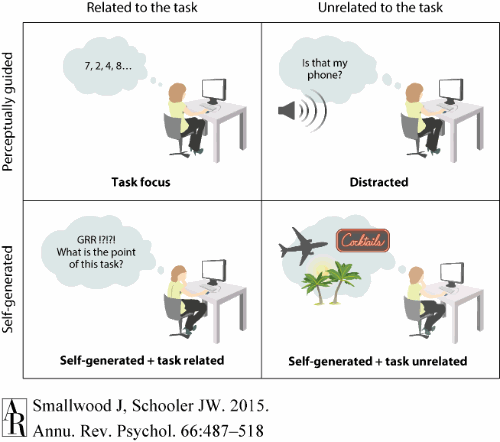
\includegraphics[width=300px]{Figures/mw_split.png}
    \caption{Perceptually vs. Self-generated and on-off task split taken from \cite{SmallwoodSchooler2015}.}
    \label{fig: mw_split}
\end{figure}
%\end{comment}

Here, off-task self-generated thought is called mind-wandering, the opposite of mindful attention. Several studies have examined mind-wandering imprint on EEG data\cite{Kam2011}. A few publicly available datasets can also be found \cite{Jin2019PredictingMW}\cite{DelormeEEGMeditationStudy}\cite{Rodriguez-Larios2020}\cite{DelormeEGGMeditationThinking}. Hence, by building on the mind-wandering literature, a device for the estimation of meditative proficiency and progress can be built.



%\section{Project description}

%This master's thesis continues the project thesis written in fall 2023 in \autoref{Appendix B}. The thesis aims to lay a foundation for studying contemplative practices using lab-grade objective measurement tools focusing on EEG and building a classification tool for estimating contemplative proficiency and progress. The thesis's main contribution to this goal is a code base for a Convolutional Neural Network classification tool built upon the EEGNeX architecture and preliminary data analysis of the study conducted in the project thesis.

\section{Scope of the Overall Project}

The primary objective of the Contemplative Neuroscience Project is to develop a method for more accurately measuring the meditation progress of novice meditators. This necessitates integrating subjective and objective measurements to provide a more comprehensive estimate of progress than either approach could achieve independently. Reliable estimates of meditation progress could be instrumental in subsequent studies to identify the most effective techniques for learning meditation. On a personal level, these estimates could offer novice meditators more precise guidance, potentially reducing dropout rates.

This knowledge is crucial for selecting specific practices to achieve desired health and wellness outcomes, which may enhance quality of life and benefits in healthcare and personal development. For example, practices that elicit parasympathetic responses, such as reduced heart rate and increased heart rate variability, can be strategically employed for relaxation, cardiovascular health, and cognitive enhancement. High-quality progress assessments could thus have practical implications for managing the stressors of modern life and addressing mental health challenges. This potential aligns with the development goals outlined in the United Nations Sustainable Development Goal 3, which aims to ensure healthy lives and promote well-being for all ages (\cite{UN_SDG3_2023}).

\begin{figure}[h!]
    \centering
    
\includegraphics[width=0.3\linewidth]{Figures/goal3.jpg}
    \caption{UN Sustainable Development Goal 3: Ensure healthy lives and promote well-being at all ages.}
    \label{fig:goal3}
\end{figure}

Several pieces need to come together to achieve this long-term goal, as shown in \autoref{fig:overal_goal}.
The first step involves gathering EEG data from novice meditators during meditation sessions. This data will be the foundation for developing and refining objective analysis tools. Regular sessions should be recorded to capture meditative experiences and mind-wandering episodes.

By utilizing the collected data, the next step is to design and build machine learning models—specifically, classification tools capable of distinguishing between states of mind wandering and focused attention. This involves training Convolutional Neural Networks (CNNs) or other suitable algorithms on the EEG data to classify the cognitive states accurately.

With the classification tools, each meditator's progression can be tracked over time. By analyzing the trends in the classification data, insights into how an individual's ability to maintain focused attention or control mind wandering evolves with practice can be drawn. This longitudinal analysis is crucial for assessing the effectiveness of the meditation practice.

To enhance the robustness of the findings, the objective data obtained from the EEG analysis should be integrated with subjective data collected through questionnaires in a triangulation format. These questionnaires can gather personal insights from the meditators about their experiences, challenges, and perceived progress, providing a comprehensive view of their meditation journey.

Finally, the comprehensive data analysis setup will be leveraged to guide individual meditators and facilitate progress analysis. Based on the trends observed in their data, specific recommendations can be made to help them optimize their practice, overcome challenges, and achieve better mental health outcomes.

\begin{figure}[H]
    \centering
    \hspace*{-2cm} 
    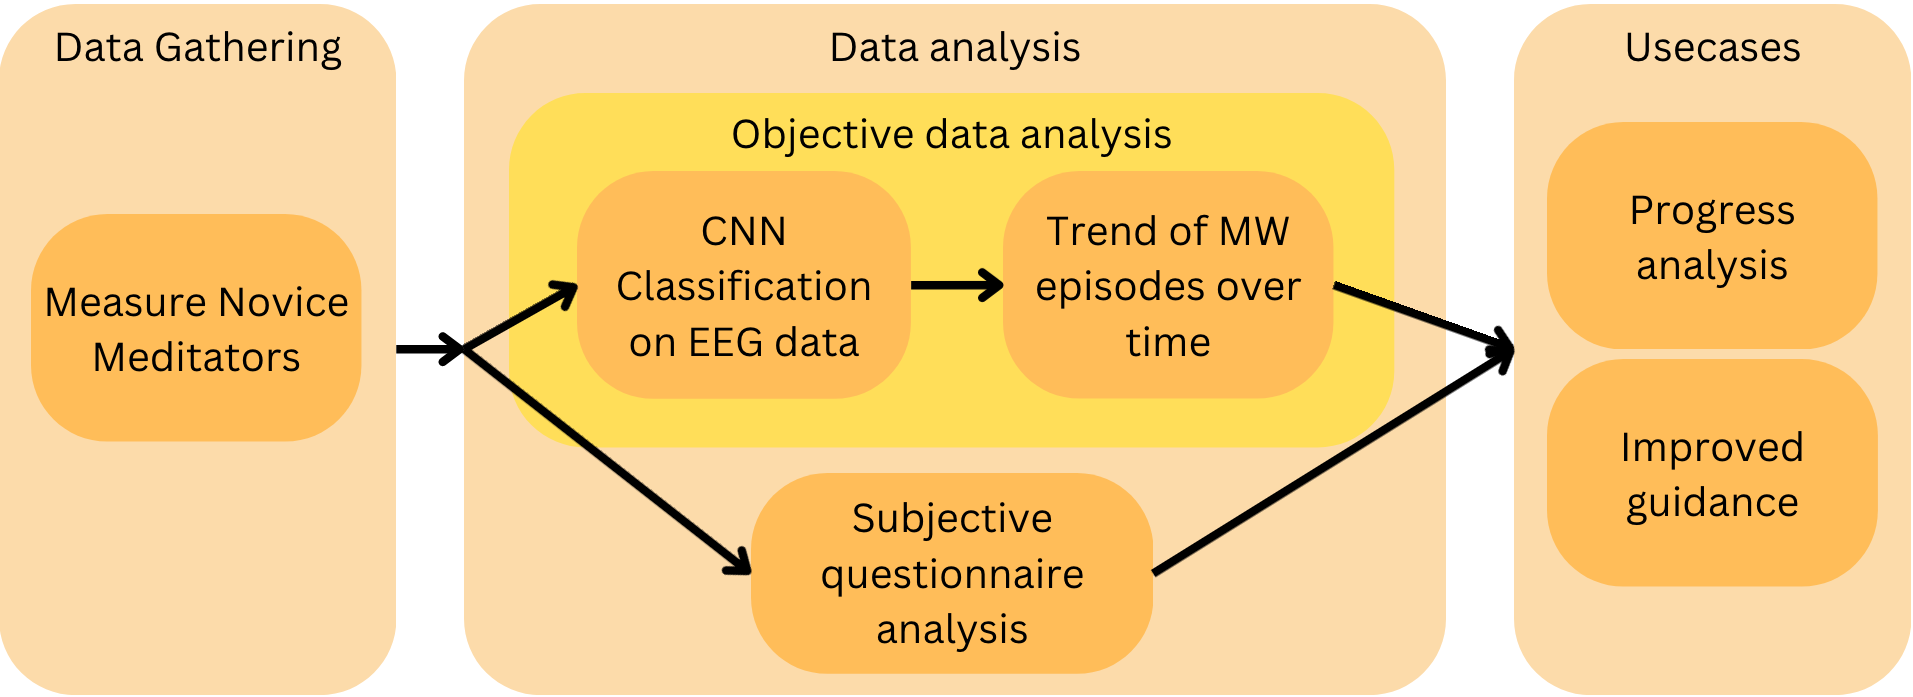
\includegraphics[width=500px]{Figures/project_flow.png}
    \caption{Overall project Goal.}
    \label{fig:overal_goal}
\end{figure}

Zooming in on the CNN classification from \autoref{fig:overal_goal}, several parts need to be implemented for the best estimates of Mind Wandering as shown in \autoref{fig:cnn_goal}. The training data for CNN can come from online datasets or be developed internally to secure high-quality data. Then, it's the CNN implementation, finding the best underlying architectures, model designs, and design choices for what parameters to include. Optimization is another significant step in parameter optimization and selecting the best channels. This could reduce time as some channels are likely more important for prediction while others give less valuable information. At last, the CNN needs to be validated on another dataset to see that it performs well on unseen data and is reliable. 

\begin{figure}[H]
    \centering
    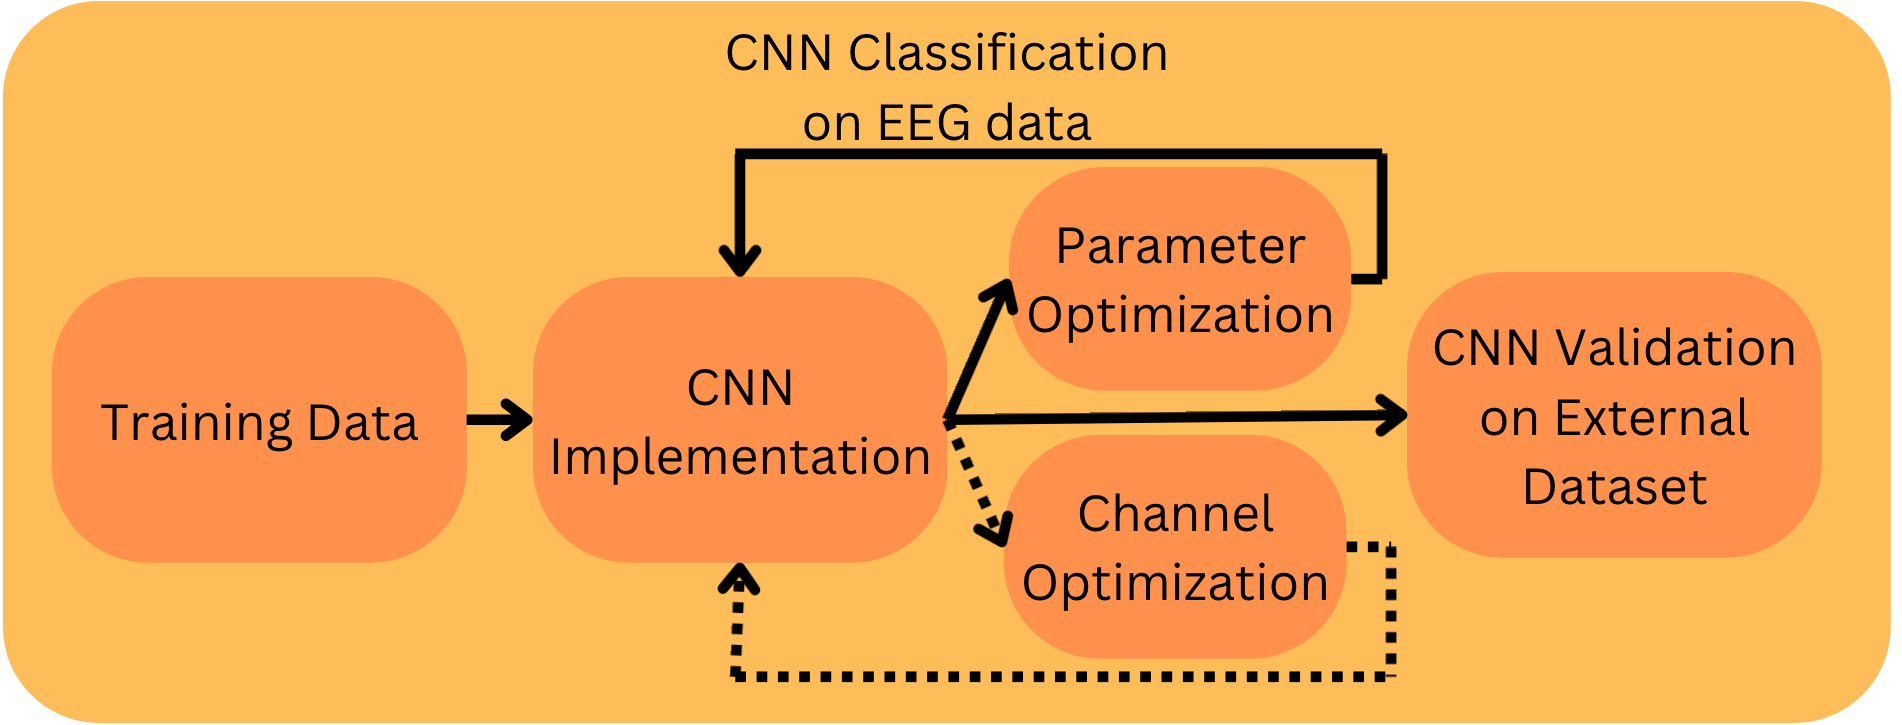
\includegraphics[width=400px]{Figures/cnn_flow.png}
    \caption{CNN Goal.}
    \label{fig:cnn_goal}
\end{figure}

\section{Scope of this Thesis}

This master's thesis builds upon the project initiated in Fall 2023 and is given in \autoref{Appendix C}. This research aims to develop and refine tools for objectively measuring contemplative practice proficiency using EEG data, focusing on crafting a robust machine-learning model. While the Project Thesis set out to collect measurements of novice meditators as they progressed, completing the Data Gathering step in \autoref{fig:overal_goal}, the primary contribution of this thesis is the development of a CNN based on the EEGNeX architecture, tailored to classify stages of contemplative proficiency and track progression over time. Hence, this thesis sets out to complete the CNN Implementation and Parameter Optimization steps in \autoref{fig:cnn_goal} and lay the groundwork for the objective data analysis step in \autoref{fig:overal_goal}. Training data collection, Channel Optimization, and CNN validation on external datasets from \autoref{fig:cnn_goal} are left for future work.

\subsection{Data Source and Model Training}
The project utilizes one of the publicly available EEG datasets, as described by \cite{Jin2019PredictingMW}. Their code can be found at \href{https://github.com/christina109/MW_EEG_CNN}{https://github.com/christina109/MW_EEG_CNN}, and the dataset can be found at \href{https://unishare.nl/index.php/s/T94LXPQqw5FEA4J}{https://unishare.nl/index.php/s/T94LXPQqw5FEA4J}. This dataset offers EEG recordings from participants engaged in tasks designed to induce and measure mind-wandering. The CNN model was trained to distinguish between 'on-task' and 'mind-wandering' states. The dataset has a dual-task framework involving both a Sustained Attention to Response Task (SART) and a Visual Search (VS) task, enabling the exploration of the classifier's task generality.

\subsection{Methodological Innovations}
Significant efforts were made to enhance the model's accuracy and generalizability:
Significant efforts were made to enhance the model's accuracy and generalizability:
\begin{itemize}
    \item \textbf{Individual and General Models}: Different CNN models were developed and tested, including personalized models for individual participants and a general model trained on the entire dataset with subsequent fine-tuning on personal data.
    \item \textbf{Data Balancing Techniques}: Various strategies were employed to address the imbalances inherent in the dataset, such as random undersampling, oversampling, and the Synthetic Minority Over-sampling Technique (SMOTE). Further innovation was introduced through the use of the Synthetic MEMD Minority Oversampling Technique (SMEMD-MOTE), specifically designed to handle the unique characteristics of EEG signals.
    \item \textbf{Noise and Artifact Reduction}: To improve data quality, unimportant Intrinsic Mode Functions (IMFs) were identified and removed, enhancing the signal clarity and, thereby, the reliability of the classification results.
\end{itemize}

\subsection{Evaluation and Results}
The effectiveness of these methodologies was rigorously tested through cross-validation within the dataset and by evaluating the model's ability to generalize across different individuals and tasks. Preliminary results indicate that the tailored CNN models, especially those undergoing individual-specific fine-tuning, show promising accuracy and task generality improvements. These models have potential applications in real-time monitoring and evaluation of mind-wandering states during various contemplative practices. While this is a promising first step, more research and data are necessary for a robust and trustworthy model.

\subsection{Aids}
Grammarly has been used in this report as a spellchecker and to rewrite sentences for clarity. Github Copilot has been used to autocomplete code and explain uncommented code by others.

The HPC system of NTNU has also been used to speed up the training of models throughout.
%\subsection{Stakeholders}


\cleardoublepage
% The clear double page command ensures that the next text page is on the right-hand side (odd page) and produces a blank page if necessary to achieve that, as all chapters should begin on the right-hand side


\chapter{Theory}

\section{Mind Wandering}
\label{sec: mind_wandering}
Mind wandering, frequently conceptualized as "task-unrelated thinking," encompasses thoughts not directly related to the task at hand \cite{Barron2011} \cite{McVay2009}. However, Smallwood and Schooler\cite{SmallwoodSchooler2015} contend that this definition is overly broad as it includes internally generated thoughts and those stimulated by external environmental cues such as sounds or visuals. In "The Restless Mind," Smallwood and Schooler propose that mind wandering occurs when executive control transitions from focusing on a primary task to engaging with personally relevant goals. They outline three core consequences of this shift: First, tasks requiring extensive controlled processing consume significant working-memory resources, reducing mind wandering due to resource limitations. Second, mind-wandering episodes may impair the processing accuracy of external stimuli as cognitive resources are redirected toward internal tasks. Third, if a hierarchical model of goals is assumed, goal-related processes may be activated automatically, allowing a secondary personal goal to supersede the primary task focus.

Empirical evidence suggests that mind wandering frequency diminishes with an increase in the rate of stimulus presentation \cite{Antrobus1968} \cite{Giambra1995} \cite{Smallwood2004}, aligning with the first outcome posited by Smallwood and Schooler. This relationship implies that the stimulus presentation rate is critical when compiling a balanced dataset for research purposes. The studies by Antrobus\cite{Antrobus1968}, Giambra\cite{Giambra1995}, and Smallwood and Davies\cite{Smallwood2004} also indicate that mind wandering increases during well-practiced tasks, suggesting that repeated experimental runs can influence the distribution of mind wandering episodes. The hypothesis that mind wandering competes for working memory resources suggests task performance will likely deteriorate during mind-wandering episodes in sufficiently resource-demanding tasks. Teasdale and Dritschel\cite{Teasdale1995} demonstrated this effect in a random-number generation task, thereby confirming that task performance can indicate mind-wandering episodes and, consequently, work as part of a method for validating experimental labels.

\section{Detection of Mindwandering}

Detection of mind wandering presents significant challenges. As noted by Smallwood and Schooler \cite{SmallwoodSchooler2015}: 
"... at least three conceptual issues arise in the investigation of mind wandering: (a) the lack of direct experimental control, (b) the covert nature of self-generated thoughts, and (c) the validity and potential reactivity of introspective evidence."

\subsection{Verbal Reporting}
Verbal self-reporting serves as a rudimentary method for detecting mind wandering. Nevertheless, the reliability of self-reports is questionable. Schooler and Schreiber have shown that self-report accuracy can be assessed by correlating them with physiological markers, providing a more comprehensive understanding of their validity\cite{Schooler2004}.

\subsection{Thought Sampling}
Thought sampling includes two primary methods: self-caught and probe-caught. In self-caught mind wandering, individuals report mind wandering upon self-recognition; hence, the measurement focuses primarily on their awareness of mind-wandering rather than the underlying frequency episodes. Conversely, probe-caught mind wandering employs a method where subjects are intermittently questioned about their current mental state during the task. Responses may be self-classified by the subjects or experimenter-classified based on predefined criteria. Probe-caught sampling thus leads to a better estimate of the actual mind-wandering frequency. However, self-classification may lead to an artificially high reporting rate of mind wandering due to increased vigilance following instructions about mind wandering characteristics \cite{Giambra1995}. It is also crucial to recognize that self-awareness might still be a limiting factor, as participants may not fully perceive their mental state, even when prompted. Despite this, self-classification offers practical advantages, such as reduced need for disclosing personal information and simplicity in self-assessment. \cite{SmallwoodSchooler2006}.

\subsection{Study design}
\label{subsec: study_design}
As previously discussed, accurately labeling mind-wandering episodes is fraught with difficulties. To enhance estimates' validity regarding individuals' true internal state, a triangulation method has been proposed \cite{SmallwoodSchooler2015}. This approach integrates self-classified and probe-caught mind-wandering reports with task performance metrics and neurophysiological data. This multidimensional strategy seeks to corroborate subjective reports through objective measures and scientific knowledge from earlier studies, thereby providing a more robust and reliable estimate of mind wandering.

The Sustained Attention to Response Task (SART) is a tool that has proven itself as robust in studying mind wandering through its ability to induce and measure lapses in attention during monotonous tasks\cite{Robertson1997}. The dual approach of combining real-time subjective experience sampling with objective performance measures, such as intra-individual reaction time variability, offers a comprehensive method to assess mind wandering accurately. This variability has been shown to predict mind wandering \cite{Baird2012}\cite{BastianSackur2013}, and such fits with the triangulation approach. 

By embedding experience-sampling probes into the SART,  datasets can be created with annotations of mind-wandering instances and subsequently validated by measurable performance metrics. The SART might be particularly suitable for settings where sustained attention is crucial and has been tested in different meditation studies using Vipassana\cite{Zanesco2013} and Mindfulness Training \cite{Morrison2014}. To further increase the validity of the labels collected, EEG Event-Related Potential (ERP) analysis has been used for SART validation\cite{Kam2011}. Thus, SART-generated data is likely to enhance the viability of datasets for predictive models in an EEG data contemplative research context, especially when validated through triangulation. 

\section{EEG Signals}
Electroencephalography, or EEG, is a method for measuring the brain's electrical activity. EEG is a non-invasive method where a set amount of electrodes are fitted to the subject's scalp in a predefined pattern, often a subset of the 10-10 system described in \autoref{fig: eeg_1010}. The electrode designs are split into dry and wet electrodes, where dry electrodes try to connect to the scalp itself. In contrast, wet electrodes use an electrically conductive gel to pass the signal from the scalp to the electrode. Each electrode, often called a channel, records a time series of electrical potentials, resulting in a data array of the number of channels times the length of the channel's time series ([n\_channel, time\_series\_lenght]). Thus, EEG recordings give a wave-like pattern over all channels, often visualized as in \autoref{fig: eeg_viz}.

\begin{figure}
    \centering
    \includegraphics[width=0.6\linewidth]{Figures/eeg/EEG_10-10_system_with_additional_information.png}
    \caption{EEG 10-10 System. Picture from \cite{Wiki1020EEG}.}
    \label{fig: eeg_1010}
\end{figure}
\begin{figure}
    \centering
    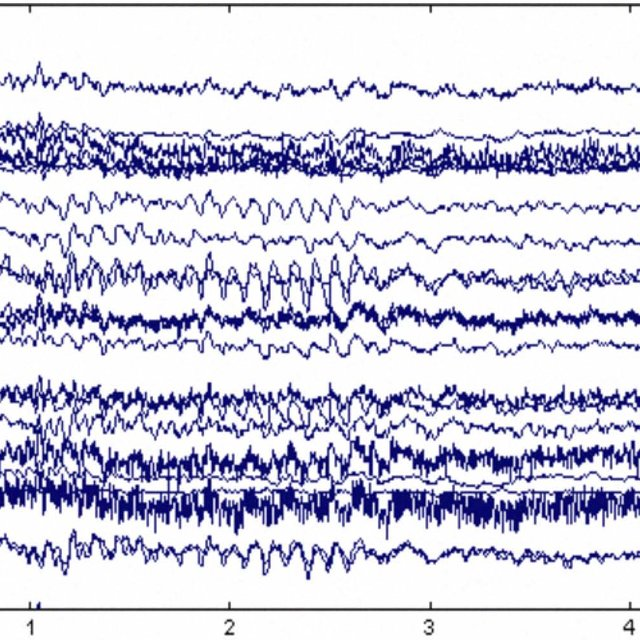
\includegraphics[width=0.6\linewidth]{Figures/eeg/eeg.jpg}
    \caption{Visualized EEG recording over several channels.}
    \label{fig: eeg_viz}
\end{figure}

\subsection{Waves}
The study of waves has a long history in the mathematical sciences, garnering interest from the likes of Newton, Maxwell, and Fourier. Fourier's seminal insight proved that any function could be represented as a series of simple sine waves. Conversely, complex waveforms can also be decomposed into these fundamental sine components, allowing the analysis of wave signals in their simplest forms\cite{bracewell1986fourier}.

\subsubsection{Empirical Mode Decompositions (EMD)}
Among the techniques for wave analysis, the Hilbert-Huang Transform (HHT)\cite{Huang1998EMD} stands out, particularly in comparison to the traditional Fourier Transform. The HHT is designed to decompose a signal into Intrinsic Mode Functions (IMFs). These IMFs are similar to the sine wave components in Fourier analysis but are specifically tailored for analyzing non-stationary signals whose statistical properties vary over time\cite{Huang1998EMD} .

A stationary process in stochastic terms is defined by statistical properties unchanging in time, such as consistent mean and variance, mathematically represented as \(F(x)\). In contrast, a non-stationary process exhibits time-dependent statistical properties, represented as \(F(x,t)\). Non-stationary signals, therefore, have a generator function that varies over time. Although all real-world signals are non-stationary to some degree, the rate of change often dictates their practical analysis\cite{Brockwell1991}. For instance, while the Moon's orbit exhibits minimal daily changes, making it practically stationary for short-term predictions, modeling its trajectory over millennia with today's parameters would yield significant inaccuracies. Contrary to the Moon's orbit, EEG signals of the brain exhibit rapid changes in the underlying generator functions, making their non-stationarity significant\cite{Klonowski2009}. 
 

\subsection{Multivariate Empirical Mode Decomposition}

The Multivariate Empirical Mode Decomposition (MEMD) represents a significant advancement in signal processing, particularly tailored for analyzing complex multidimensional signals\cite{Mandic2013}. This algorithm is an extension of the classical one-dimensional Empirical Mode Decomposition (EMD)\cite{Huang1998EMD}, designed to address the limitations of applying EMD separately to each channel of multidimensional data. Unlike the conventional approach, MEMD considers the interconnectedness of data channels, which is crucial for accurately interpreting signal information.

A practical illustration of MEMD's necessity can be observed in neuroscientific applications, such as analyzing neural signals captured by several electrodes over a cluster of neurons. Signals recorded from such clusters are influenced by both the spatial arrangement of the electrodes and the varying conductive properties of the intervening biological tissues. As a result, each electrode captures a signal that, while unique in timing and amplitude due to the distance and tissue permeability from the neural source, is fundamentally linked to the same originating neural event. The traditional EMD, if applied individually to each signal channel, would fail to capture these interdependencies, potentially leading to misleading conclusions about the neural activity.

MEMD, therefore, provides a more holistic view of multidimensional data by recognizing and preserving the intrinsic relationships among the channels. This makes it indispensable for accurately decomposing complex signals into their constituent IMFs.

\section{Introduction to Machine Learning}

Machine learning is a substantial field within computer science, which is distinguished by teaching computers the ability to learn from and make decisions based on data\cite{Mohammed2016}. This thesis will concentrate on the specific aspects of machine learning crucial for understanding the project's framework and the rationale behind critical decisions.

\subsection{Differentiating Machine Learning from Traditional Programming}

Traditional programming involves the creation of explicit, rule-based algorithms that instruct the computer on solving specific types of problems. This method is highly effective for a range of applications; however, it encounters limitations when the complexity of the problems increases, such as when rules must scale significantly\cite{Mohammed2016}. For instance, consider the challenge of identifying the number of fingers displayed in an image or classifying handwritten digits from the MNIST dataset\cite{deng2012mnist}. As illustrated in \autoref{fig: mnist2}, handwritten digits like the number "2" can vary significantly in shape and style, posing a substantial challenge for rule-based systems.

\begin{figure}
    \centering
    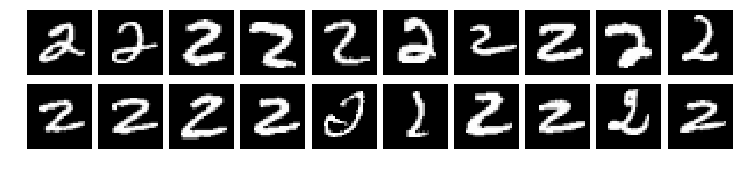
\includegraphics[width=250px]{Figures/MLintro/mnist2.png}
    \caption{Variations of the handwritten digit '2' from the MNIST dataset}
    \label{fig: mnist2}
\end{figure}

Humans can typically recognize these variations effortlessly, suggesting that a different approach is feasible for machines. This approach involves features, a distinct and recognizable element of the input data that forms a complete picture when combined with other features. Features can be engineered manually but can also be learned automatically from data, a foundational machine learning principle. As depicted in \autoref{fig: fromProgrammingToML}, the difference between traditional programming and machine learning involves shifting from manually coded instructions to systems that learn from data to identify and utilize features\cite{Mohammed2016}.

\begin{figure}
    \centering
    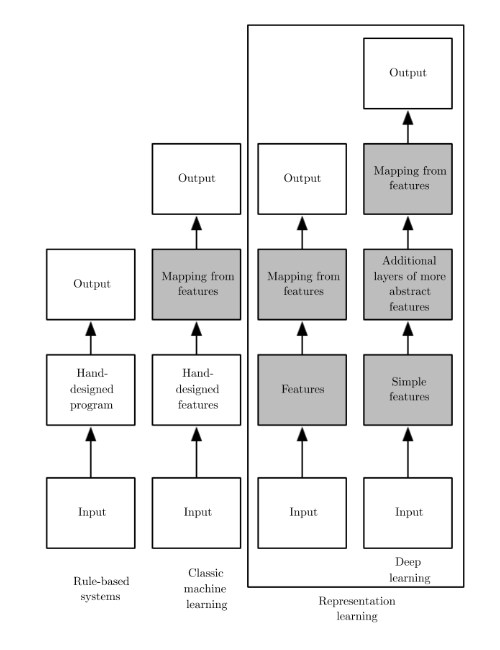
\includegraphics[width=250px]{Figures/MLintro/ml.png}
    \caption{Transition from standard programming to machine learning, highlighting components that are learned from data. Source: hyperlink: Modeling with neural networks slide 1}
    \label{fig: fromProgrammingToML}
\end{figure}

\subsection{Neural Networks and Features}

Neural networks are comprised of interconnected units known as nodes, organized into distinct layers. These layers include the input layer, which receives the initial data, and the output layer, which provides the final classification or prediction. Between these, there may be several intermediate layers. Networks with many such layers are described as deep, whereas those with few are termed shallow\cite{Sarker2021}. Each node in these networks is assigned a value between 0 and 1, and connections between nodes, known as edges, are weighted. These weights, which influence the strength of the connections, are adjustable through learning processes and are crucial for the network's ability to solve specific problems\cite{Witten2005}.

\begin{figure}
    \centering
    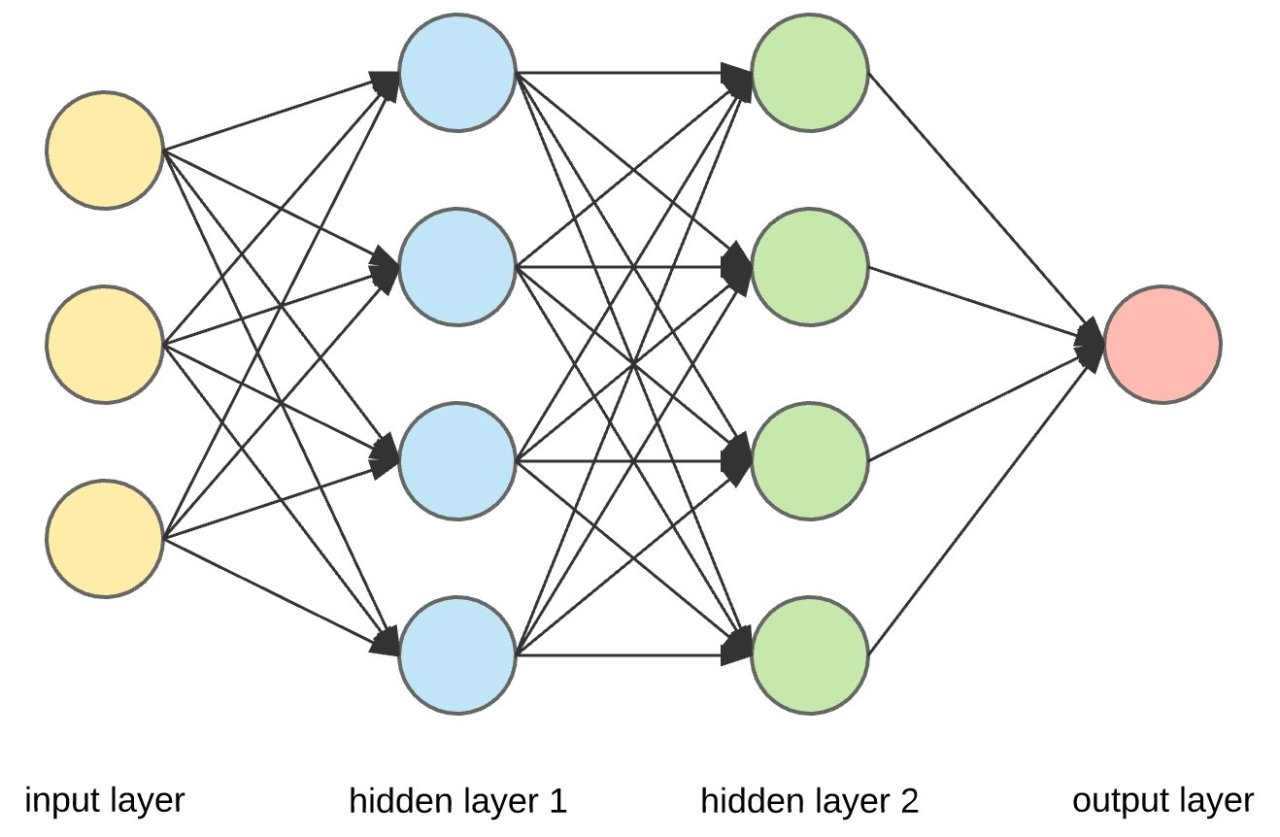
\includegraphics[width=250px]{Figures/MLintro/nn.jpg}
    \caption{Illustration of a fully connected neural network, where each node in one layer is connected to all nodes in the subsequent layer.}
    \label{fig: nn2ex}
\end{figure}

As shown in \autoref{fig: nn2ex}, the depicted neural network processes an input, such as a hand-drawn number "2." The first layer consists of nodes representing different features identifiable in various parts of the digits. Each node compares its encoded features against the input to generate a similarity score ranging from 0 to 1. Nodes not resembling any features in the input receive lower scores. Subsequent layers synthesize the information from prior layers to progressively refine the interpretation and combination of features, culminating in a final output that identifies the most likely digit represented by the input.

This example simplifies and leaves out many of the complexities inherent in neural network operation, the relevant ones of which will be addressed in detail in subsequent sections of this thesis. A critical aspect of neural networks is that their features are learned directly from data. Consequently, while a network can learn to identify common characteristics in differently drawn "2s", the specific reasons why certain features are deemed significant remain unclear. This opacity can introduce challenges, particularly in interpreting how the network makes its decisions\cite{Mohammed2016}.

\subsection{Data Integrity}
The reliability of a neural network is heavily contingent upon the data quality used during training\cite{Sarker2021}. Since weights and features within a neural network are derived from examples, poor-quality or non-representative data can significantly impair the network's performance. For instance, if all images of cats in the training set are associated with a blue sky, the model might erroneously learn to associate the presence of a blue sky with cats. This hypothetical underscores the necessity of a large and diverse dataset to ensure the neural network can generalize well from its training and function effectively in real-world conditions.

\subsection{Training a Neural Network}
Training a neural network involves adjusting the weights to predict known outcomes accurately. This process is conducted by presenting the network with numerous examples and iteratively modifying the weights based on the network's accuracy. The degree of error in the network's predictions is quantified using a metric known as the loss function. To optimize the learning process, an algorithm known as the optimizer guides the adjustments of weights, aiming to reduce the loss as efficiently as possible. Proper data partitioning is also critical to avoid overfitting, where a network might perform well on training data but poorly on unseen data. Although each of these components, loss function, optimizer, and data partitioning, are complex subjects worthy of detailed study, this thesis will provide only a concise overview, focusing on their roles in training neural networks.

\subsubsection{Loss Functions}
\label{subsubsec: loss_functions}
A loss function quantifies the discrepancy between predicted values by the network and their true values, serving as a critical component in training neural networks. The design of the loss function significantly influences learning dynamics by prioritizing certain types of errors over others\cite{Ciampiconi2023}. For instance, the Mean Absolute Error (MAE) and the Mean Squared Error (MSE) approach errors differently: MAE evaluates the absolute difference, leading to linear error sensitivity, whereas MSE squares the differences, disproportionately penalizing more significant errors. This characteristic of MSE makes it particularly effective in situations where considerable errors are unacceptable.

\[
\text{MAE} = \frac{1}{n} \sum_{i=1}^{n} |y_i - \hat{y}_i|
\]
\[
\text{MSE} = \frac{1}{n} \sum_{i=1}^{n} (y_i - \hat{y}_i)^2
\]

\subsubsection{Optimizers}
Optimizers adjust the network's weights to minimize the loss function. The process involves navigating a high-dimensional landscape defined by the loss function to find a point of minimal error, akin to finding the lowest point in a valley. A popular optimizer, ADAM, functions similarly to a ball rolling down a hill, using momentum to escape shallow local minima and gravitate towards more optimal solutions\cite{Ruder2016}. The initial position in this landscape significantly influences the effectiveness and speed of the optimization process.

\subsubsection{Data Splitting}
Informative testing of a neural network's performance requires careful data management and can be attained by splitting data into training, validation, and testing sets\cite{Joseph2020}. This strategy prevents 'data leakage,' where adjustments to the model are influenced by the test set, leading to inflated performance metrics that do not generalize to new data. The training set is used to fit the model, the validation set is used to tune model parameters, and the test set provides an unbiased model evaluation. While adjusting hyperparameters based on test set performance is not uncommon, this can lead to subtle forms of data leakage, decreasing the accuracy of the generalizability estimate. An ideal data splitting strategy, as shown in \autoref{fig: datasplitt}, minimizes these risks by ensuring that only the validation data influence model tuning. 
\begin{figure}
    \centering
    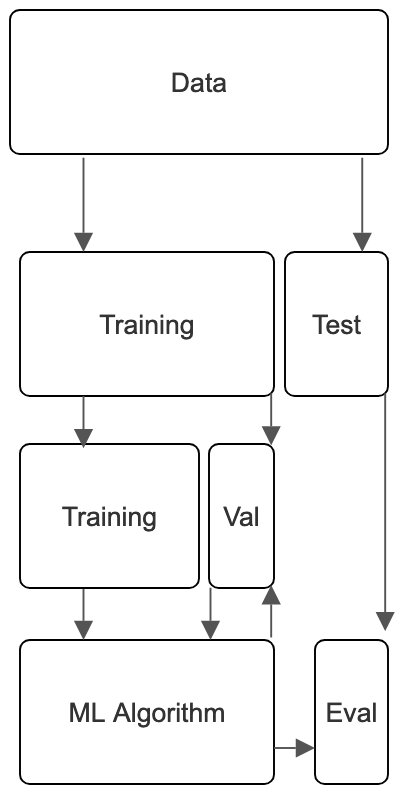
\includegraphics[width=150px]{Figures/MLintro/data_split.png}
    \caption{Idealized data splitting schema for training machine learning algorithms}
    \label{fig: datasplitt}
\end{figure}

\subsection{Overfitting}
\label{subsec: overfitting}
In machine learning, overfitting is the phenomenon where a model learns the training data too closely and subsequently fails to generalize to new, unseen data. An overfitted model can be conceptualized as one with more parameters than can be justified by the available data or that is necessary to explain it\cite{Valdenegro-Toro2022}. Mathematically, these parameters are analogous to the degree of a polynomial. The essence of overfitting is that the model inadvertently captures the noise in the data, mistaking it for the underlying data structure. This is exemplified in \autoref{fig: overfitting}.

\begin{figure}
    \centering
    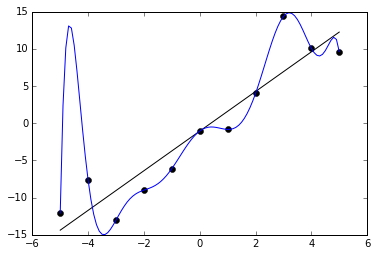
\includegraphics[width=400px]{Figures/Overfitted_Data.png}
    \caption{Demonstration of Overfitting for noisy linear data. The black dots are the data points, the black line is the linear data structure, and the blue line is the overfitted model of the data structure.}
    \label{fig: overfitting}
\end{figure}


\section{Learning paradigms}
\subsection{Supervised Learning}
Supervised learning is characterized by the use of labeled data, where each input, such as an image of a dog, is paired with a corresponding text label, in this case, "dog"\cite{Sarker2021}. The learning algorithm improves its predictions over time by adjusting weights based on the accuracy of previous predictions. This method requires a substantial volume of correctly labeled data, which can be challenging and time-consuming.

\subsection{Unsupervised Learning}
In contrast, unsupervised learning operates without labeled data, focusing instead on discovering intrinsic patterns and relationships within the dataset\cite{Sarker2021}. Not relying on predefined labels might enable the algorithm to uncover hidden structures in the data. However, this strength also introduces complexity in interpretation, as the algorithm may prioritize unexpected or non-intuitive patterns. For instance, it might cluster images based on similarities in background elements rather than distinguishing features of the subjects, such as grouping all animals photographed on grass together instead of grouping them as cats and dogs.

While this method significantly reduces the necessity for extensive labeled datasets, it demands a thorough understanding of the underlying domain to interpret and utilize the results appropriately. The potential for the algorithm to focus on irrelevant similarities poses a challenge, requiring careful analysis to ensure that the derived categorizations align with meaningful and practical insights into the data.

\section{Convolutional Neural Networks}

Due to their unique architecture, Convolutional Neural Networks (CNNs) have become a cornerstone in image classification. This architecture effectively separates feature extraction from image classification\cite{LeCun1998-CNN} as exemplified in \autoref{fig: cnn}.

\subsection{Feature Extraction Using Kernel Convolution}
CNNs utilize convolutional layers to process input images. These layers employ kernels, or small matrices, that systematically apply their weights across the image to extract features\cite{LeCun1998-CNN}. This process demonstrated in \autoref{fig: kernelconv}, involves sliding the kernel over the image and computing the dot product at each position, which emphasizes specific features like edges or textures depending on the kernel's configuration.

\begin{figure}
    \centering
    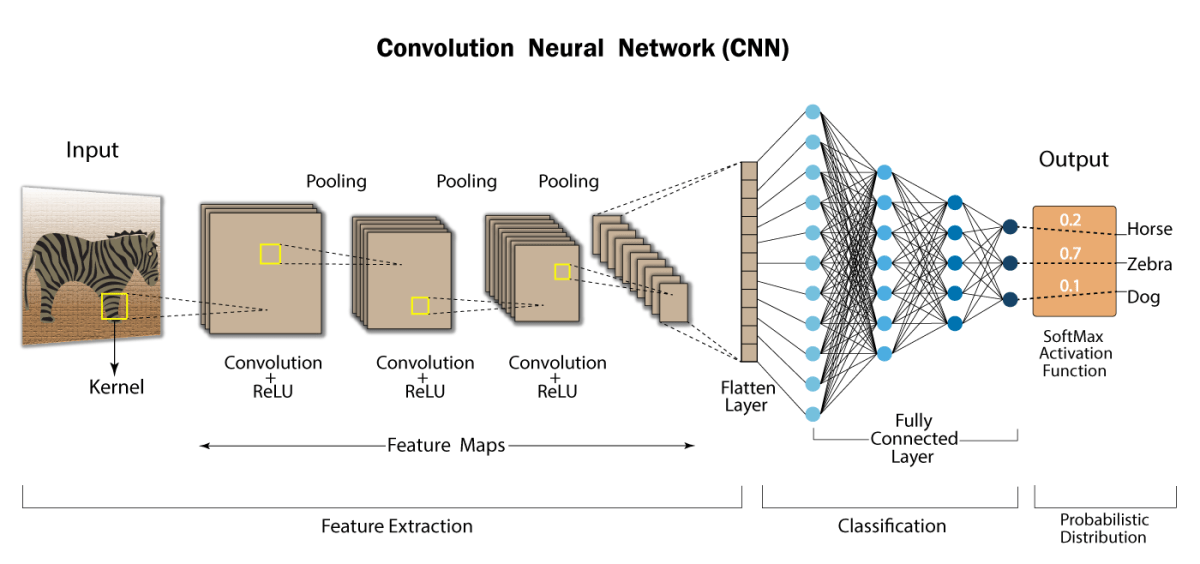
\includegraphics[width=400px]{Figures/MLintro/cnn.png}
    \caption{Visual explanation of a CNN architecture, highlighting the flow from feature extraction to classification.}
    \label{fig: cnn}
\end{figure}
\begin{figure}
    \centering
    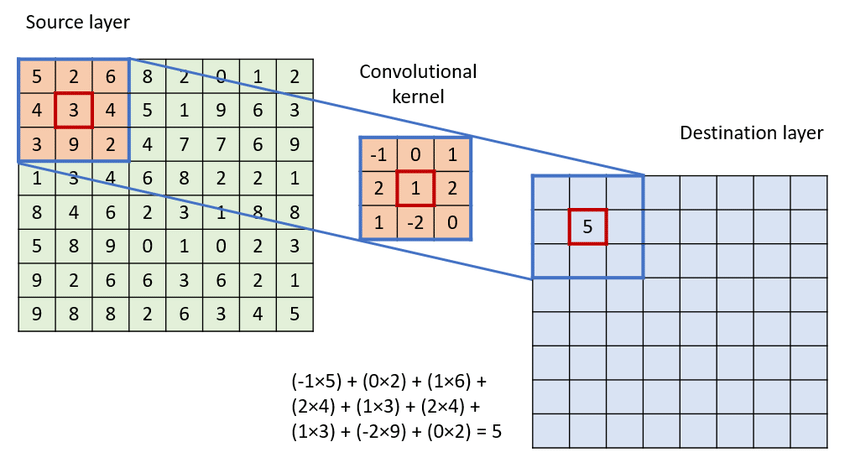
\includegraphics[width=400px]{Figures/MLintro/kernelConv.png}
    \caption{Demonstration of kernel convolution across a grayscale image to detect features.}
    \label{fig: kernelconv}
\end{figure}

For instance, a vertical line-detecting kernel might be structured as follows: 
\[
\text{Vertical Line Detecting Kernel} = 
\begin{bmatrix}
-1 & 0 & 1 \\
-1 & 0 & 1 \\
-1 & 0 & 1
\end{bmatrix}
\]
This kernel highlights vertical transitions between bright and dark regions since a vertical edge in a black-and-white image will be dark on one side and bright on the other, leading to a large number when going from dark to bright and a large negative number when going from bright to dark. This edge capturing is crucial for understanding the structure within images. By changing the structure of the kernels, different features in the image can be detected. For instance, the transpose of the Vertical Line Dection Kernel would detect horizontal lines. Crucially, the kernels are learned during the training process, not predefined, as explained here.

\subsection{Classification Using a Classic Neural Network}
After feature extraction, the subsequent layers of the CNN combine these features to form more complex representations, leading to the final classification layer. These layers are similar to traditional neural networks and integrate extracted features to effectively predict the image's content, ensuring the model generalizes well to unseen data.



\section{CNNs in the Context of EEG}
EEG signals are characterized by their complexity and non-stationary nature, presenting unique challenges in signal processing. CNNs are particularly well-suited for addressing these challenges due to their capability to handle complex data structures with the convolutional layers enabling the detection of intricate patterns within the EEG data, such as low-frequency transients, which are prominent in these signals\cite{Chen2023}.

One effective technique in enhancing CNN's performance with EEG data is the application of Continuous Wavelet Transformation (CWT). CWT transforms EEG signals into scalograms, visual representations that capture time and frequency information \cite{Arts2022}. This transformation allows CNNs to effectively localize different frequency components over time, thereby improving the detection and classification of various cognitive activities. This feature is especially beneficial given the frequent presence of artifacts and noise in EEG recordings, which can obscure critical information.

The advent of advanced CNN models such as EEGNeX marks a significant improvement in this domain \cite{demir2022eegnext}. EEGNeX has demonstrated enhanced accuracy and generalizability in classifying cognitive activities, surpassing other leading models like EEGNet\cite{Lawhern_2018}. It achieves this by effectively utilizing the spectral and temporal information inherent in EEG signals, providing a more nuanced interpretation of neural activities.

\section{Preprocessing}
Preprocessing in EEG analysis is crucial for enhancing the clarity of the signals by minimizing noise and irrelevant artifacts, which can confuse the classifier.

\subsection{IMF Selection}
\label{subsec: img_selection}
A proposed noise and artifact removal method in EEG signals involves IMF Selection, which uses the MEMD algorithm to decompose the signal into IMFs. The IMFs are then evaluated based on their Euclidean distance from the original signal, and only the \(n\) IMFs closest to the original signal are retained. This process produces a cleaner version of the original signal when recombined. An even more involved IMF selection algorithm was presented by \cite{SinghMoore2023}. There are two primary variations of the Euclidian version used in this thesis: 

\subsubsection{Individual Optimization Variation}
This variation optimizes each channel within each epoch independently, retaining only the most significant IMFs for clarity. Although this approach aims to maximize the signal cleanliness for improved classification results, it risks potential issues if IMFs across different epochs are later interchanged. Such swapping could lead to synthetic signals not representative of the underlying biological phenomena.

\subsubsection{Cross-Epoch Consistent Optimization Variation}
An alternative strategy is maintaining consistency in the IMFs selected across all epochs. This is achieved by analyzing a representative sample of epochs to determine the most important IMFs on average and retaining these for all data. This approach is less prone to errors related to IMF swapping and reduces computational complexity since it does not require optimization for every single epoch and channel. However, it risks slightly compromising the performance due to less tailored noise and artifact removal.

\subsection{Regularization}
\label{subsec: regularization}
Regularization methods are different techniques developed to reduce models' natural tendency to overfit the training data\cite{TIAN2022146}. As explained in \autoref{subsec: overfitting}, overfitted models tend to have more parameters than are necessary to understand the data. Fighting this is key in many regularization methods.

\subsubsection{L1}
\(L_1\) regularization, also known as Lasso (Least Absolute Shrinkage and Selection Operator), is a technique used to prevent overfitting by adding a penalty to the loss function. This penalty is proportional to the absolute values of the model's coefficients. The primary objective of \(L_1\) regularization is to induce sparsity in the model. Sparsity means that the model uses fewer features, as \(L_1\) regularization drives some of the coefficients to exactly zero. This effectively removes unimportant features, reducing the dimensionality and leading to better performance. The \(L_1\) can be considered analogous to the MAE form \autoref{subsubsec: loss_functions}.

\subsubsection{L2}
\(L_2\) regularization, also known as Ridge regression, is a technique used to prevent overfitting by adding a penalty to the loss function. This penalty is proportional to the square of the coefficients of the model. Unlike \(L_1\) regularization, which can drive some coefficients to zero, \(L_2\) regularization tends to shrink the coefficients towards zero but not exactly to zero. This approach helps retain all features while reducing their influence, which can lead to more stable and balanced models. The \(L_2\) can be considered analogous to the MSE form \autoref{subsubsec: loss_functions}.

\subsubsection{Dropout}
Dropout is a different kind of regularization technique designed to enhance neural networks' generalization capability. The method works by randomly deactivating a subset of neurons within the network, effectively nullifying their contribution during the training process. The proportion of neurons to be deactivated is determined by a hyperparameter known as the Dropout Rate. This rate can be fine-tuned to achieve optimal performance tailored to specific tasks. 

For instance, a Dropout Rate of 0.5 implies that 50\% of the neurons are randomly set to zero during each training iteration. The primary objective of this technique is to mitigate overfitting by preventing the network from becoming overly reliant on particular neurons. This encourages the network to develop distributed representations focusing on more robust features that are useful across different subsets of data, reducing the risk of overfitting and enhancing generalization.

\subsubsection{Early Stopping}
\label{subsec: early_stopping}
Early stopping is a regularization technique used to prevent overfitting during the training process. This method involves monitoring the model's performance on a validation set and halting the training process when the performance ceases to improve.

In practice, the training of a neural network typically involves iterating over the dataset multiple times, each iteration being called an epoch (not to be confused with epochs from neuroscience and MNE used later). During each epoch, the model's parameters are updated to minimize the loss function, improving its performance on the training data. However, if training continues for too long, the model may start to overfit.

Early stopping addresses this issue by using the validation set. After each epoch, the model's performance is evaluated on the validation set using a chosen metric, such as validation loss or accuracy. If the validation performance does not improve for a predefined number of consecutive epochs, the training process is stopped. The number of consecutive epochs it takes before stopping is called the Patience and is a tunable hyperparameter. Early stopping thus ensures that the model parameters are saved where the model performs best on the validation set, likely achieving a better generalization to unseen data.

\section{Data Augmentation}
Data augmentation is a process by which additional data is generated from existing data through modifications and transformations. These techniques often involve altering images by rotation, blurring, or other means to create variations while maintaining the core characteristics of the original data. Such artificially created data, called synthetic data, effectively enhances the dataset without needing new real-world data\cite{wang2024comprehensive}.
\subsection{Augmentation Ratio}
\label{subsec: augmentation_ratio}
The augmentation ratio is how much additional data should be added as synthetic data. A higher ratio results in more data, but the synthetic proportion also increases. The formula is: 

\begin{equation}
\text{synthetic\_data\_len} = \text{len(real\_data)} \times \text{augmentation\_ratio}
\end{equation}

Thus, a ratio of 1.0 will mean 50\% of the total data is synthetic. 

\section{Unbalanced Datasets}
\label{unbalanced_dataset_theory}
A significant challenge in supervised learning is the uneven distribution of classes within datasets. Predominant classes can bias the model to favor the majority class, undermining the model's ability to learn from less frequent classes. For instance, in a binary classifier where one class constitutes 95\% of the data, a model predicting this majority class exclusively would achieve a 95\% accuracy despite not genuinely discerning the underlying patterns distinct to each class but instead relying solely on the class distribution.

\subsection{Data Balancing Methods}
To mitigate the effects of class imbalance, several strategies have been developed\cite{10061154}: 

\subsubsection{Undersampling}
Undersampling involves randomly removing instances from the majority class to equalize the class distribution. This method directly reduces the volume of data, potentially eliminating valuable information, but it avoids creating synthetic data and duplicating existing data.

\subsubsection{Oversampling}
In contrast, oversampling increases the representation of the minority class by duplicating its instances. This method preserves valuable data from the majority class but risks overfitting, as it increases the likelihood of the model learning noise and specific patterns from the duplicated minority class examples.

\subsubsection{Synthetic Minority Oversampling Technique (SMOTE)}
SMOTE enhances dataset balance through synthetic data generation for the minority class. This technique selects a random instance \(A\) from the minority class, identifies its \(k\) nearest neighbors, chooses one neighbor \(B\), and generates a new sample \(C\) based on a point along the line segment connecting \(A\) and \(B\) in feature space. SMOTE alleviates the duplication issue prevalent in traditional oversampling but can produce ambiguous class boundaries if class distributions overlap significantly. The creation process does not account for majority class characteristics, which might lead to less effective learning in areas where classes intersect \cite{smote}.

\subsubsection{Class Weight Balancing}
Class weight balancing adjusts the impact of each class during the training process based on its representation. Classes with fewer samples are given higher relative importance, calculated using the formula: 
\[
\frac{n_{\text{samples}}}{n_{\text{classes}} \cdot \text{np.bincount}(y)}
\]
Here, \(n_{samples}\) refers to the total number of samples, \(n_{classes}\) the number of classes, and \(np.bincount(y)\) gives the number of samples in each class.
This method effectively increases the model's sensitivity to the minority class without altering the data distribution.

\subsubsection{Synthetic MEMD Minority Oversampling Technique (SMEMD-MOTE)}
SMEMD-MOTE is tailored for EEG signal datasets and uses synthetic data generation to balance classes. It involves selecting two random samples, decomposing them into their respective IMFs, swapping some of their IMFs, and recombining these to form a new, synthetic signal within the same class. This technique builds on the principles of SMOTE and is adapted to EEG data analysis's unique characteristics and requirements.


\section{Testing Model Performance}
\label{performanceMetrics}

This section outlines some metrics used to evaluate the effectiveness of machine learning binary classifiers\cite{rainio2024evaluation}.

\subsection{Accuracy}
Accuracy is the most intuitive performance measure, and it is simply a ratio of correctly predicted observations to total observations. It is useful when the target classes in the dataset are nearly balanced. Accuracy is calculated as: 
\[
\text{Accuracy} = \frac{\text{Number of correct predictions}}{\text{Total number of predictions}}
\]

\subsection{Precision}
Precision (also called positive predictive value) is the ratio of correctly predicted positive observations to the total predicted positives. It can be an essential measure in scenarios where the cost of a false positive is high.
\[
\text{Precision} = \frac{\text{True Positives}}{\text{True Positives + False Positives}}
\]

\subsection{Recall}
Recall (also known as sensitivity) is the ratio of correctly predicted positive observations to all observations belonging to the positive class. Thus, it measures how many of the objects in the positive class were labeled correctly.
\[
\text{Recall} = \frac{\text{True Positives}}{\text{True Positives + False Negatives}}
\]

\subsection{F1 Score}
The F1 Score is the weighted average of Precision and Recall. Therefore, this score takes both false positives and false negatives into account. It is beneficial when the classes are imbalanced. The F1 score is the harmonic mean of precision and recall: 
\[
\text{F1 Score} = 2 \cdot \left(\frac{\text{Precision} \cdot \text{Recall}}{\text{Precision + Recall}}\right)
\]

\subsection{AUROC}
The Area Under the Receiver Operating Characteristic curve (AUROC, sometimes AUC) represents the measure of the ability of the model to distinguish between the classes. An AUROC of 0.5 suggests no discriminative ability (chance), while 1.0 represents perfect discrimination and 0.0 is inverse discrimination. For a binary classification model (“OT” vs. “MW”), the AUROC tells you the probability that a randomly selected “OT” class member will have a higher predicted probability of being classified as “OT” than a randomly selected “MW” image.

\subsection{Kappa}
The Kappa statistic (or Cohen's Kappa) measures the prediction agreement with the true values. It is normalized by the imbalance of the classes in the data, making it more reliable when classes are unbalanced. The Kappa statistic considers random chance in the accuracy calculation, providing a more nuanced understanding of model performance.
\[
\text{Kappa} = \frac{P_o - P_e}{1 - P_e}
\]
Where \(P_o\) is the relative observed agreement among raters (i.e., accuracy), and \(P_e\) is the hypothetical probability of chance agreement.

Each metric provides unique insights into the model's performance, enabling a comprehensive evaluation beyond simple accuracy. 

\cleardoublepage


\chapter{Materials and Methods}
\section{Dataset}

\subsection{Dataset Explanation}
The dataset utilized for training the neural networks was collected and described in the study by Jin et al. (2019) \cite{Jin2019PredictingMW}. This dataset was generated during an experiment where participants engaged in two distinct attention-demanding tasks designed to induce mind wandering: a Visual Search (VS) task and a Sustained Attention to Response Task (SART).

\paragraph{Task Descriptions}
In the VS task, participants were required to identify specific shapes amongst various nontarget shapes, demanding sustained visual attention and pattern recognition. The SART involved responding to text cues displayed on a screen, where participants had to press buttons corresponding to the words' uppercase or lowercase nature. The SART was structured to present nontargets more frequently, further challenging the participants' sustained attention.

\paragraph{Mind Wandering Probes}
During these tasks, participants were intermittently prompted with questions to self-report their level of attention and cognitive state. These probes aimed to classify the participants' mental state in real time, with responses immediately recorded and timestamped. The classification from these responses was used to label the EEG data, facilitating the subsequent analysis focused on mind wandering. The specific questions used in the probes and their corresponding classifications are detailed in \autoref{tab:probe}.

\paragraph{Window Length Parameter}
A key variable in the data processing was the 'Window Length,' which defines the duration in seconds before each probe, during which EEG data were considered relevant for the corresponding mental state label. This parameter was adjustable, allowing for an exploration of the trade-off between including more EEG data for model training and maintaining a high precision in the temporal correlation between the data and its labels. Increasing the window length provided more data but potentially reduced the accuracy of the label applicability over that extended period.

\begin{table}[h]
\centering
\caption{Classification of Mental States During Task Performance}
\begin{tabular}{|c|p{8cm}|c|}
\hline
\textbf{No.} & \textbf{Probe Question} & \textbf{Classification} \\ \hline
1 & I entirely concentrated on the ongoing task. & On Task (OT) \\ \hline
2 & I evaluated aspects of the task (e.g., my performance or how long it takes). & On Task (OT) \\ \hline
3 & I thought about personal matters. & Mind Wandering (MW) \\ \hline
4 & I was distracted by my surroundings (e.g., noise, temperature, my physical condition). & Distracted (DS) \\ \hline
5 & I was daydreaming, thinking of task unrelated things. & Mind Wandering (MW) \\ \hline
6 & I was not paying attention, but my thought wasn't anywhere specifically. & Unclear (UC) \\ \hline
\end{tabular}
\label{tab:probe}
\end{table}

\subsection{Preprocessing}
The initial preprocessing steps were conducted using MATLAB, following the procedures outlined by Jin et al. (2019) \cite{Jin2019PredictingMW}. 

Following the initial preprocessing in MATLAB, further data processing, encompassing additional preprocessing tasks, model development, and subsequent analyses, was executed in Python. A key aspect of Python-based preprocessing was the refinement of EEG data through the selective exclusion of less significant Intrinsic Mode Functions (IMFs). This approach involved retaining only the \(n\) most significant IMFs that closely resembled the original signal's profile, with \(n\) being an adjustable parameter. This parameterization facilitated targeted noise and artifact mitigation, enhancing data quality.

Additionally, data balancing techniques were applied to address class imbalance issues inherent in the dataset. A subsequent section of this thesis provides detailed descriptions of the data balancing methods utilized.

\subsubsection{MNE Epoch Data Structure}
For effective data handling, the EEG recordings were transformed into the MNE-Python Epochs data structure, henceforth referred to simply as "epochs." Each epoch comprises a segment of the total data captured within a predefined window. Specifically, a 12-second window preceding each probe, and an associated label derived from the participant's response to the probe. To facilitate a binary classification between 'On Task' (OT) and 'Mind Wandering' (MW), responses categorized under 'Distracted' (DS) and 'Unclear' (UC) were excluded. Furthermore, the epochs were systematically organized into a dictionary indexed by the subject from whom the data were collected. Leading to the following main datastructure:

\begin{verbatim}
all_epochs = {
    1: mne.Epochs(data1, events1, event_id),
    2: mne.Epochs(data2, events2, event_id),
    3: mne.Epochs(data3, events3, event_id),
    ...
}
\end{verbatim}

where 1,2,3 etc. correspond to the subject numbers containing their respective epochs. This structure made it easy to implement Leave-One-Participant-Out (LOPO), Leave-N-Participants-Out (LNPO) and individual modeling and training later on. The data is the raw EEG data for the epochs, events are the probe answer for each epoch. The data and events are extracted from the open dataset using the "load\_dataset\_n\_tasks" function provided by Jin et al. \cite{Jin2019PredictingMW}. Event\_id is the translation from internal events numbering to the classification and is thus the same for all subjects, in our case:

\begin{verbatim}
event_id = {
    0: 'ot',
    1: 'mw'
}
\end{verbatim}

\subsection{Data Splitting}
Data division into testing, validation, and training subsets was established at the project's outset. This initial split was performed before any class balancing or data augmentation processes to ensure that the validation and test sets more accurately mirrored the true distribution of the underlying data. However, this approach led to an imbalance in the dataset, which inadvertently biased the models toward predicting based on class distribution rather than the intrinsic data characteristics.

To address these biases, a revised strategy was implemented where the test set continued to reflect the actual data distribution. In contrast, the validation set was balanced between classes to mitigate the influence of class distribution on model selection. This adjustment presented challenges, namely the choice between undersampling the majority class, losing valuable data, or oversampling the minority class, causing duplication for the validation set. The approach taken was defaulting to undersampling to avoid overfitting yet leaving it as an option for later testing. 

\subsection{Class Balancing}
Given the significant imbalance between the classes in the dataset, various class balancing techniques were implemented to mitigate the model's predisposition to favor the majority class, which could compromise the accuracy of predictions based on actual data characteristics rather than class distribution. Five class balancing methods were explored: Undersampling, Oversampling, Synthetic Minority Over-sampling Technique (SMOTE), Synthetic MEMD Minority Oversampling Technique (SMEMD-MOTE), and a baseline scenario with no balancing applied. Each method's theoretical basis and application are detailed in \autoref{unbalanced_dataset_theory}. Importantly, the balancing interventions were applied exclusively to the training dataset to ensure the model's generalization ability from a balanced learning environment.

\subsection{Data Augmentation}
A data augmentation technique was also explored to further enhance the model's robustness and performance. The technique involved integrating synthetic data into the training set, thereby increasing its size and diversity. The specific augmentation method utilized was based on the technique used in SMEMD-MOTE, which is designed to generate data that maintains the intrinsic properties of the original signals while providing new variations designed to fit well with EEG signals. 



\subsection{Regularization}

In machine learning, regularization techniques are critical for controlling model complexity and preventing overfitting, particularly in models with large feature spaces. Overfitting occurs when a model learns not only the underlying pattern but also the noise in the training data, leading to poor generalization on unseen data. To address this, this study evaluated three regularization techniques: L1 regularization, L2 regularization, and a control scenario with no regularization applied.

\begin{itemize}
    \item \textbf{L1 Regularization}: This method, also known as Lasso regularization, encourages the model to consider only the most important features by effectively reducing the less significant feature weights to zero. It is particularly useful for feature selection in models with high dimensionality.
    \item \textbf{L2 Regularization}: Known as Ridge regularization, this technique penalizes the square of the feature weights, which helps control the model's complexity without eliminating the weights entirely. It tends to distribute the error among all the features equally and is useful in cases where many features are believed to contribute to the predictive power of the model.
    \item \textbf{No Regularization}: The model's performance without any regularization was also assessed to establish a baseline, allowing for a comparative analysis of the impact of L1 and L2 regularization on model complexity and performance.
\end{itemize}

\section{Model Designs}
\subsection{Individual Model}
In the individual model design, each subject got their model trained specifically on them. Each model was then tested on the test epochs from the same subject to see how well it was classified within subjects. Due to early testing results, this model design was abandoned early on.
\subsection{General Model}
In the general model design, the model was trained on all except one participant, the Leave-One-Participant-Out (LOPO) method. It was then tested on the left-out subject to see how well it generalized across different subjects. This was repeated for all subjects, leaving out a different subject every time.
\subsection{Transfer Model}
The last model design was a mix of the first two; a general model was created on all but one subject, and then the general model was fine-tuned on the left-out subject and tested on unseen epochs from this subject. Due to time constraints, this design was only developed in code but not well tested, and so it is left for future work. 

%%%%%
\section{Configuration Exploration}
This thesis explored various configurations for the Convolutional Neural Network (CNN) to optimize performance and generalizability. A Python module named `config` was developed to manage the general setup configurations and CNN-specific parameters. This module was split into two parts: `config.py` for general settings and `neural\_net\_config.yaml` for CNN-specific settings.

\paragraph{config.py}
This file primarily facilitated the integration of High-Performance Computing (HPC) resources, simplifying the project's continuation for other students. It included high-level configurations such as HPC user configurations, job names, folder structures, and high-order settings.

\paragraph{neural\_net\_config.yaml}
The CNN-specific parameters were organized using a YAML structure due to its flexibility with data types and its ability to include comments, enhancing the explainability of the configuration settings and making onboarding to the project easier. The YAML file contained a dictionary specifying possible configurations for the CNNs, structured with key-value pairs where the values were lists of configuration options. Below is an excerpt from this configuration dictionary:

\begin{footnotesize}
\begin{verbatim}
common:
  time: ["05:00:00"]  # Run time for the job on HPC (Idun)
  partition: ["GPUQ"]  # Choose between CPU and GPU
  mem: ["64GB"]  # Memory needed
  model_to_use: ["EEGNeX"]  # ["EEGNeX", "EEGnet2018"], Only models listed here will be run
  
# Model specific parameters
model:
  EEGNeX:
    mode: ["general"]  # ["individual", "general", "transfer"]
    transfer_model_sub: [null]  # If mode is transfer, specify the subject for fine-tuning
    batchSize: [30]
    nEpoch: [100]  # Number of complete passes through the training dataset
    balanceMethod: [null, "oversample", "smote", "undersample", "memd"]
    dropout: [0.4]  # Dropout rate
\end{verbatim}
\end{footnotesize}
Each key in the dictionary represents a configuration parameter with mutually exclusive options. The configurations were dynamically combined into separate runs, called jobs, each testing a unique combination of settings.

\section{HPC Integration}
\label{hpcIntegration}
Due to the extensive computational demands of training CNNs, a module was developed to facilitate using NTNU's HPC device, IDUN. This module enabled interactions with IDUN directly from the Visual Studio Code environment, allowing for job submission, monitoring, and retrieval of outputs. It automated the translation of configurations from the `config` module into HPC-compatible `.slurm` files and managed the distribution of tasks across the computing resources.

\section{Results Generation}
Upon retrieval, results from various configurations needed to be analyzed and visualized in a manner that allowed for direct comparison to assess the impact of individual parameters. A results analysis method was developed to automatically identify and group jobs differing only in one parameter, facilitating a clear comparison of their effects. The performance metrics used for evaluation included accuracy, precision, recall, F1 score, AUROC, and kappa, detailed in \autoref{performanceMetrics}. These metrics were plotted for training, validation, and test datasets, with lines indicating random chance for reference.

Furthermore, all model outputs were consolidated into a central CSV file, enhancing data analysis capabilities through visualization tools and simplifying the synthesis of results across all experimental runs.
 

\cleardoublepage


\chapter{Results}
%\section{CNN Individual Model}
%\section{CNN General Model}
%\section{CNN Transfer Model}
\section{Explanation}
\label{sec: results_explanation}

Due to time constraints, only the General Model has been extensively tested. All results presented in this thesis were generated using the General Model with the LOPO validation and test method. This means all models were trained on 28 subjects, validated on one, and tested on one. Thus, all test and validation scores are generated on subjects different from the models that were trained on, hence being across-subject scores that display the generalizability of the model. 

\subsection{Plot Explanation}
\paragraph{Scatterplot} Different plot types will be displayed in this thesis's results, including the scatter plot. The plot marks one point for each model run and shows the trends over the various models with different parameter tunings. It is impossible to see the impact of specific parameters. However, broader trends in the data might appear more clearly.

\paragraph{Metric-Set plot} The Metric-Set plot compares different values for one parameter of other metrics and on various sets. The metrics used are Accuracy, precision, recall, F1, AUROC, and Kappa in this order, and they are then repeated for each of the training, Validation, and test sets in this order. The random chance value of 0.5 for all metrics except Kappa and the random chance value of 0.0 for Kappa are plotted for convenience. The metric markers are set at the average value of all models for the particular parameter value, while the vertical line with horizontal line edges signifies one standard deviation. The small horizontal lines not connected to the vertical line represent the minimum and maximum values any model achieves for that parameter value. Plots without this standard deviation vertical line signify the best models a specific metric selects for a particular set. The chosen ones for this thesis are 'test\_kappa', 'test\_auroc', 'val\_kappa', and 'val\_auroc', meaning the Kappa and AUROC metrics for the Test and Validation sets. 

\section{Set Correlation}

\autoref{fig: test_corr_no_reg} shows the correlation between Accuracy and other metrics for the test set. A close fit to the y=x midline indicates a high correlation, while a more spread-out scatter indicates a lower correlation. The plot shows a high correlation between Accuracy and F1 and recall but a lower correlation for Kappa and AUROC. Each subplot is plotted below and zoomed in for easy inspection.
\begin{figure}[H]
    \centering
    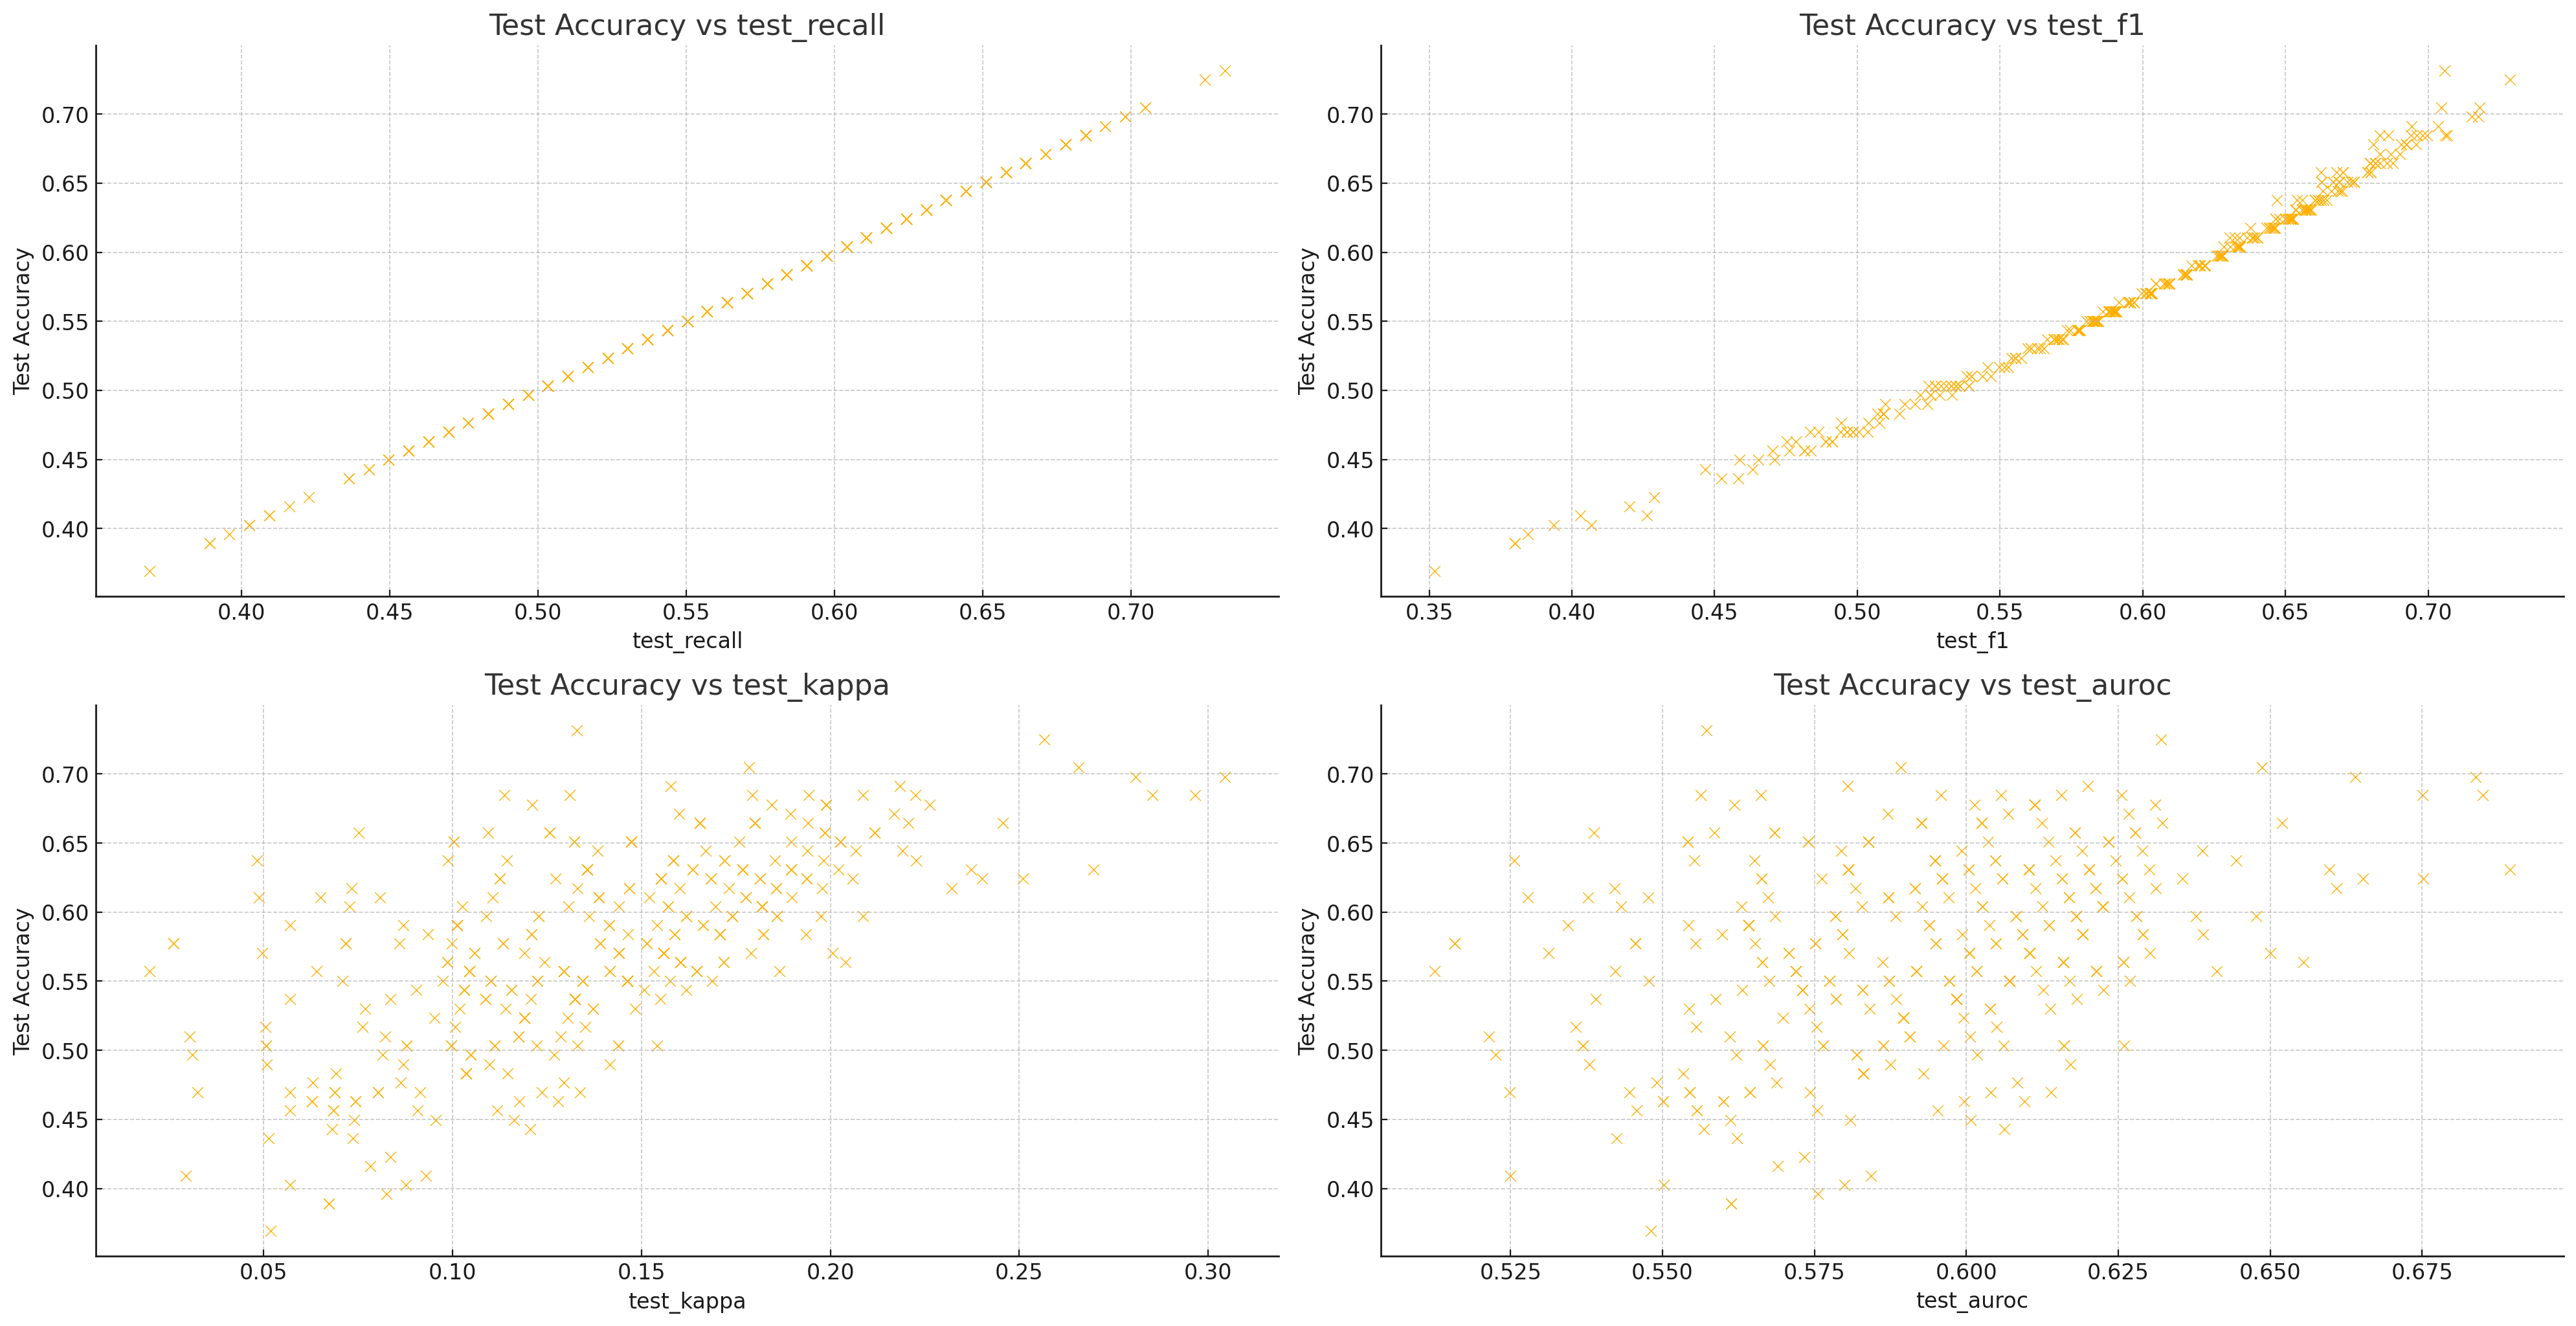
\includegraphics[width=400px]{Figures/results/acc_corr_no_reg.png}
    \caption{Scatter plot of test accuracy's correlation with other metrics for various models.}
    \label{fig: test_corr_no_reg}
\end{figure}

\autoref{fig: test_corr_no_reg_part_1} shows a zoomed-in version of the top left corner of \autoref{fig: test_corr_no_reg}. It shows the correlation between the Accuracy and Recall metrics on the Test set. The diagonal y=x line indicates perfect correlation. The correlation between the two sets is very high.
\begin{figure}[H]
    \centering
    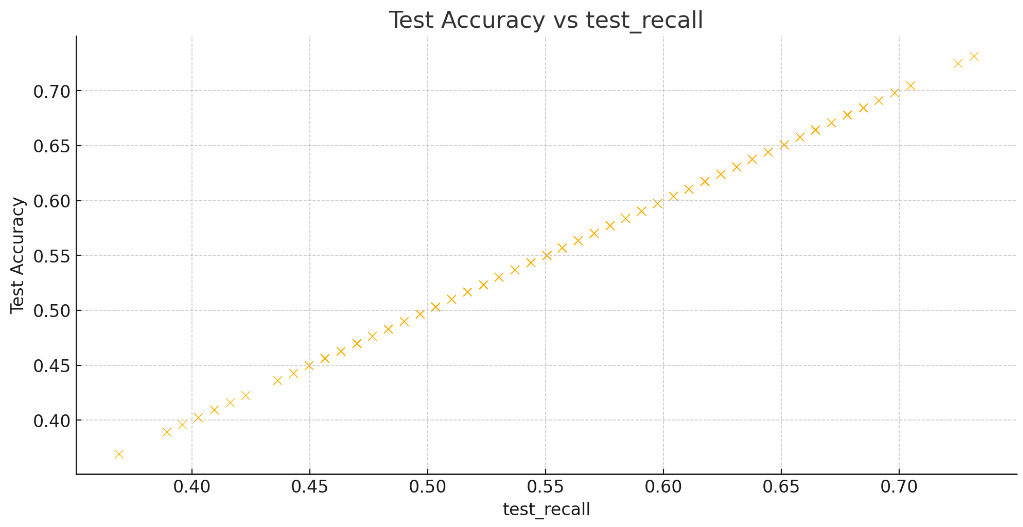
\includegraphics[width=0.9\textwidth]{Figures/results/acc_corr_no_reg_part_1.png}
    \caption{Test Accuracy vs Test Recall.}
    \label{fig: test_corr_no_reg_part_1}
\end{figure}

\autoref{fig: test_corr_no_reg_part_2} shows a zoomed-in version of the top right corner of \autoref{fig: test_corr_no_reg}. It shows the correlation between the Accuracy and F1 metrics on the Test set. The diagonal y=x line indicates perfect correlation. The correlation is lower than in \autoref{fig: test_corr_no_reg_part_1} but still high. The F1 score tends to be higher than the Accuracy, as seen from the points below the y=x line.

\begin{figure}[H]
    \centering
    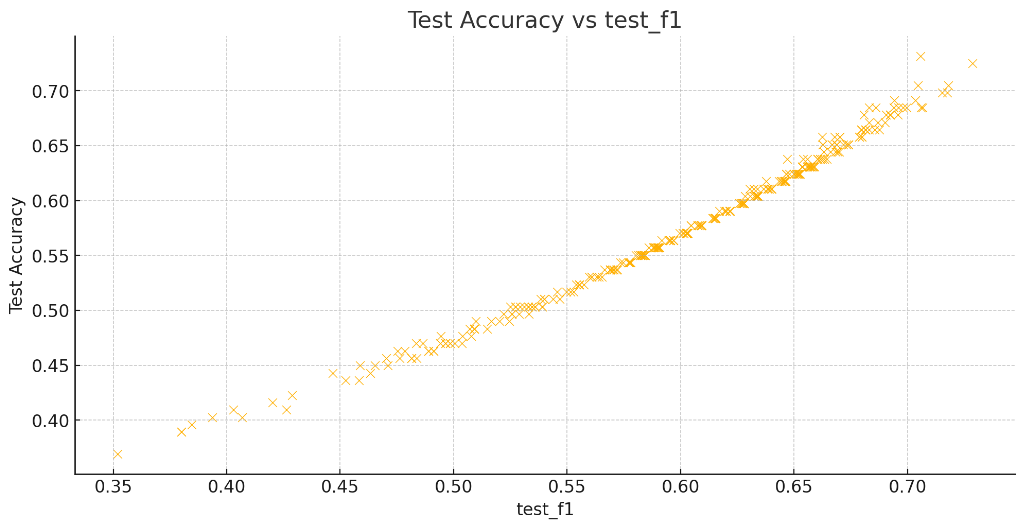
\includegraphics[width=0.9\textwidth]{Figures/results/acc_corr_no_reg_part_2.png}
    \caption{Test Accuracy vs Test F1.}
    \label{fig: test_corr_no_reg_part_2}
\end{figure}

\autoref{fig: test_corr_no_reg_part_3} shows a zoomed-in version of the lower left corner of \autoref{fig: test_corr_no_reg}. It shows the correlation between the Accuracy and Kappa metrics on the Test set. A diagonal line still indicates perfect correlation, but since Kappa's chance value is 0.0 and Accuracy's chance value is 0.5, we expect a bias term of 0.5. From the plot, it's clear that there is a positive correlation between them, but the relationship is less clear than the other plots. A Kappa of 0.05 (barely above chance) has corresponding Accuracy values from about 0.35 (inverted classifier) to about 0.65.

\begin{figure}[H]
    \centering
    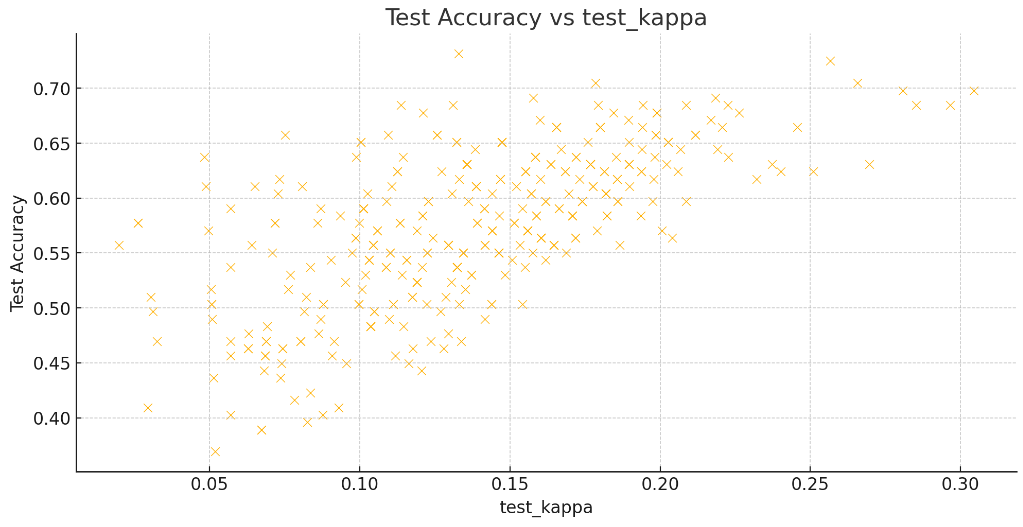
\includegraphics[width=0.9\textwidth]{Figures/results/acc_corr_no_reg_part_3.png}
    \caption{Test Accuracy vs Test Kappa.}
    \label{fig: test_corr_no_reg_part_3}
\end{figure}

\autoref{fig: test_corr_no_reg_part_4} shows a zoomed-in version of the lower right corner of \autoref{fig: test_corr_no_reg}. It shows the correlation between the Accuracy and AUROC metrics on the Test set. A diagonal line still indicates perfect correlation. The plot shows a positive correlation, but the relationship is less clear than in the top plots. 
\begin{figure}[H]
    \centering
    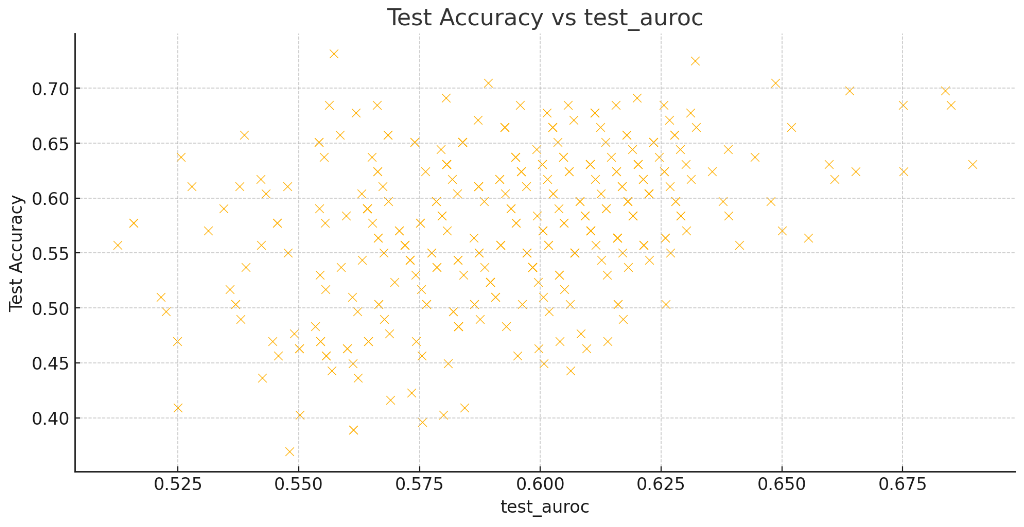
\includegraphics[width=0.9\textwidth]{Figures/results/acc_corr_no_reg_part_4.png}
    \caption{Test Accuracy vs Test AUROC.}
    \label{fig: test_corr_no_reg_part_4}
\end{figure}


\autoref{fig: reg_type_scatter} compares different regularization techniques and the correlation between various sets. Points close to the y=x line indicate a well-adjusted model, while points closer to the training or validation sets indicate overfitting to these sets. L1 and l2 suggest that the L1 and L2 regularization methods were used, respectively, while None means no regularization was applied. Each subplot is plotted below and zoomed in for easy inspection.
\begin{figure}[H]
    \centering
    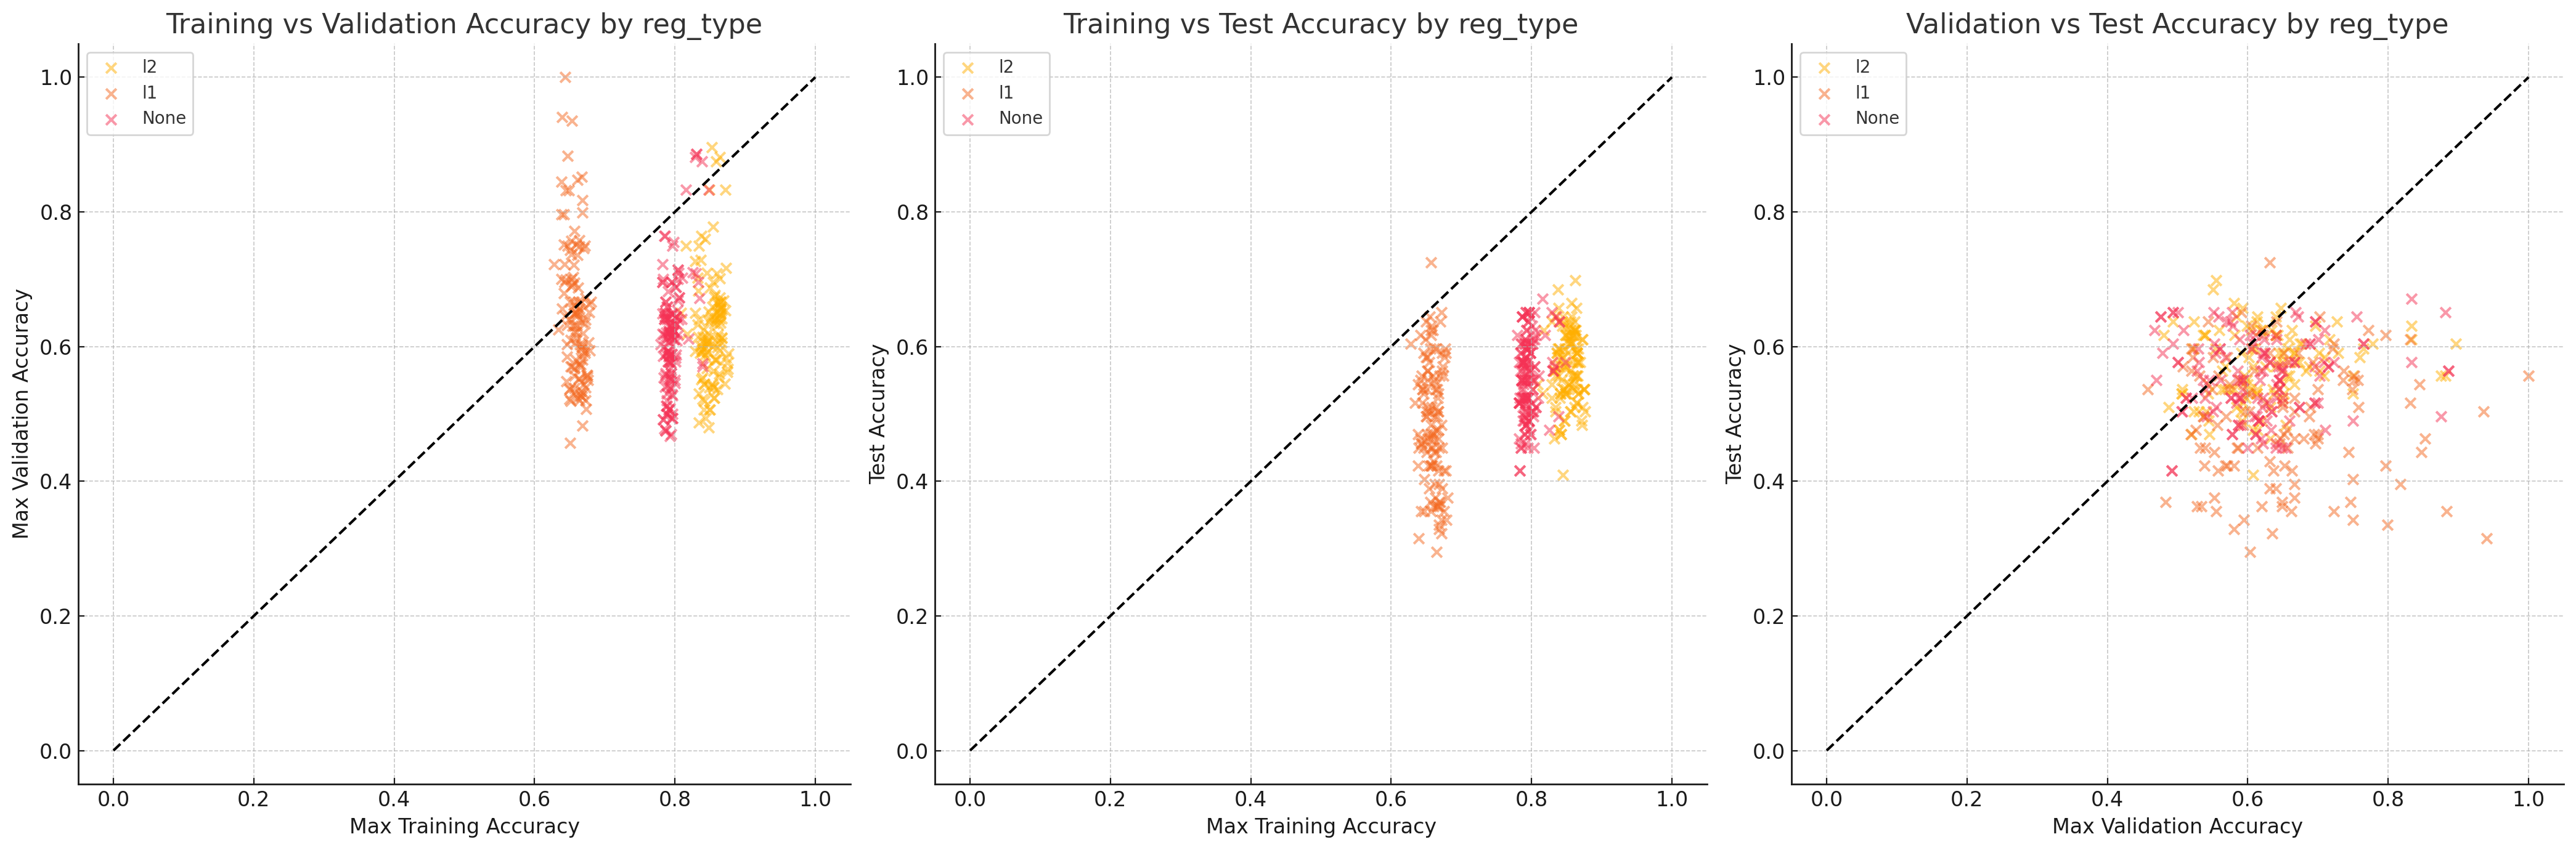
\includegraphics[width=400px]{Figures/results/scatter_reg_type.png}
    \caption{Scatter plot comparing the results of different regularization techniques on the different sets.}
    \label{fig: reg_type_scatter}
\end{figure}

\autoref{fig: reg_type_scatter_part_1} shows a zoomed in version of the left plot in \autoref{fig: reg_type_scatter}. The plot shows every model's highest accuracy score on the training and validation sets collected using their regularization method. A point along the diagonal line indicates an equal score on both sets, meaning the model generalizes well between the sets. A point below the line indicates that the model scored higher on the Training set, while above the line, the score was highest on the Validation set. From the plot, most models scored higher on the Training set. The L1 models never scored above 0.7 on the Training set, and the highest L1 score on the diagonal was just below 0.7. While L2 and None tend to score higher on the Training set, the models scoring highest on the diagonal line scored about 0.85 for L2 and 0.82 for None.

\begin{figure}[H]
    \centering
    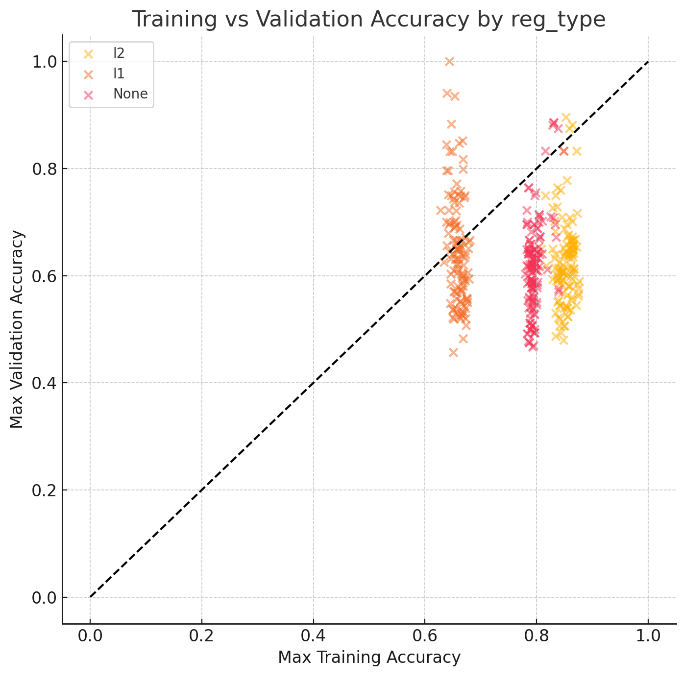
\includegraphics[width=0.7\textwidth]{Figures/results/scatter_reg_type_part_1.png}
    \caption{Training vs Validation Accuracy by reg\_type.}
    \label{fig: reg_type_scatter_part_1}
\end{figure}

\autoref{fig: reg_type_scatter_part_2} shows a zoomed in version of the middle plot in \autoref{fig: reg_type_scatter}. The plot shows every model's highest Accuracy score on the Training and Test sets collected by their regularization method. A point along the diagonal line indicates an equal score on both sets, meaning the model generalizes well between the sets. A point below the line indicates that the model scored higher on the Training set, while above the line, the score was highest on the Test set. From the plot, it's clear that most models scored higher on the Training set, with only one model scoring higher on the Test set. Only the L1 method has some models close to the diagonal. However, they also tend to score lower on both sets.

\begin{figure}[H]
    \centering
    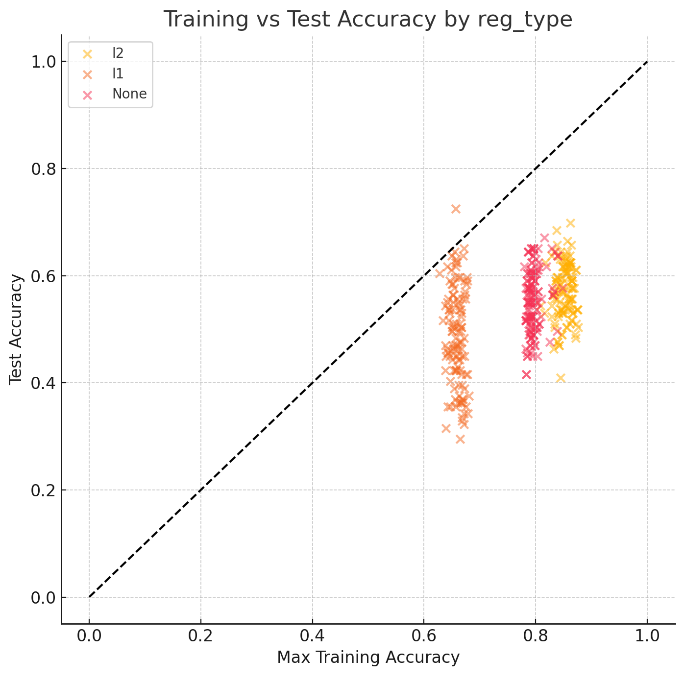
\includegraphics[width=0.7\textwidth]{Figures/results/scatter_reg_type_part_2.png}
    \caption{Training vs Test Accuracy by reg\_type.}
    \label{fig: reg_type_scatter_part_2}
\end{figure}

\autoref{fig: reg_type_scatter_part_3} shows a zoomed in version of the right plot in \autoref{fig: reg_type_scatter}. The plot shows every model's highest Accuracy score on the Validation and Test sets collected by their regularization method. A point along the diagonal line indicates an equal score on both sets, meaning the model generalizes well between the sets. A point below the line indicates that the model scored higher on the Validation set, while above the line, the score was highest on the Test set. From the plot, it's clear that most models scored higher on the Validation set, with only some scoring higher on the Test set. The correlation between the sets is higher than between the Training and Test sets, and the regularization methods are not as clustered. The L1 models are more spread out and tend to score lower on the Test set. The models scoring highest on the diagonal use the None and L2 method, scoring about 0.65.

\begin{figure}[H]
    \centering
    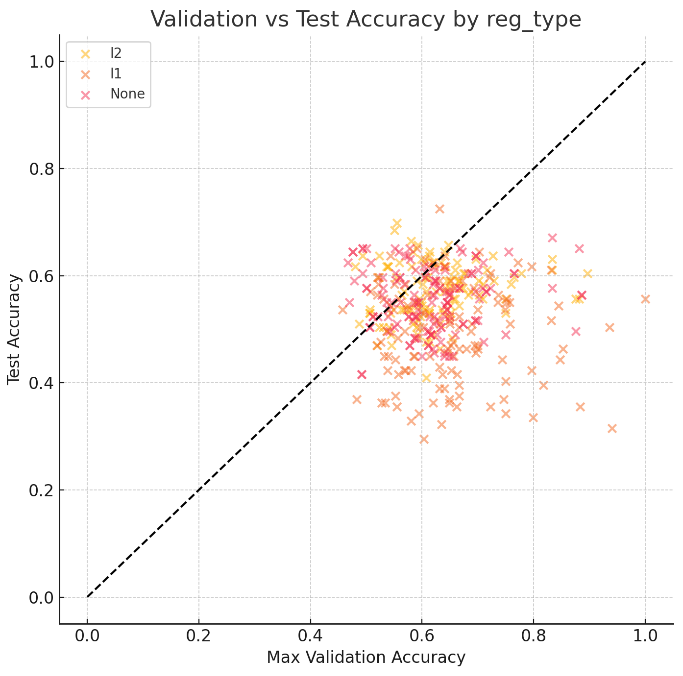
\includegraphics[width=0.7\textwidth]{Figures/results/scatter_reg_type_part_3.png}
    \caption{Validation vs Test Accuracy by reg\_type.}
    \label{fig: reg_type_scatter_part_3}
\end{figure}


\section{Balance Validation Set}
\label{res_sec: balance_val}
The Balance Validation Set parameter is a boolean value that selects whether the Validation set is balanced. A True value means that the Validation set is balanced using undersampling, meaning the majority of class epochs are deleted until there are equally many for both classes. A False value means this undersampling does not happen, and the natural imbalance is maintained in the set. 

In \autoref{fig: balance_val}, the difference statistics between different Balance Validation parameter values are compared on the three sets. On average (indicated by the marker), the False value scores better on the Training and Validation Sets but worse on the Test set for most metrics. The standard deviations (indicated by the vertical lines with short horizontal lines at the caps) seem similar for most metrics to the two parameters. The True parameter value appears to have the highest maximum values (topmost horizontal line) and the lowest minimum values (bottommost horizontal line) for most metrics on most sets.


\begin{figure}[H]
    \centering
    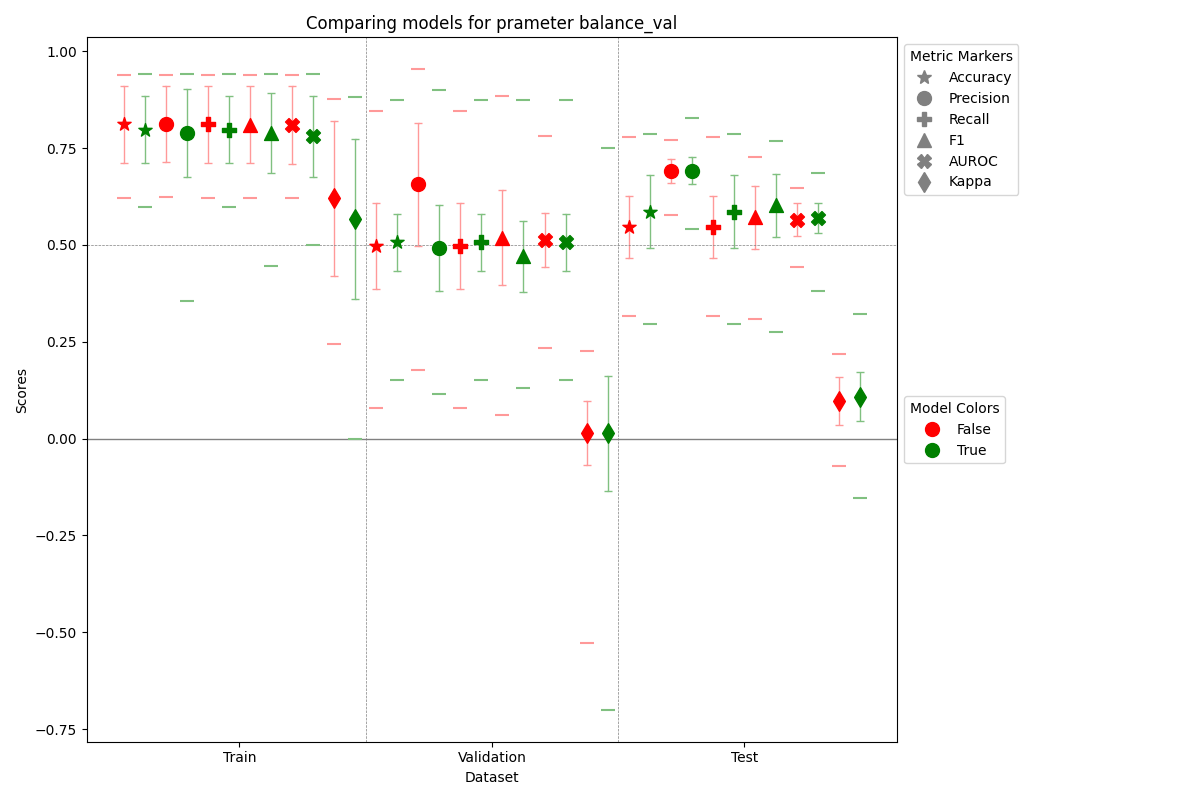
\includegraphics[width=400px]{Figures/results/balance_val/balance_val.png}
    \caption{All models compared by the Balance Validation parameter, a true value signifies an undersampling of the Validation set to have an equal amount of each class.}
    \label{fig: balance_val}
\end{figure}

In \autoref{fig: balance_val_test_auroc}, the Balance Validation parameters are plotted for the models scoring the best on the Test set metric AUROC. This means that there are only two models plotted. The True value model scored significantly better on almost all sets' metrics. The correspondence between the sets is also high, with a low but consistent drop in scores from Training to Validation to Test.


\begin{figure}[H]
    \centering
    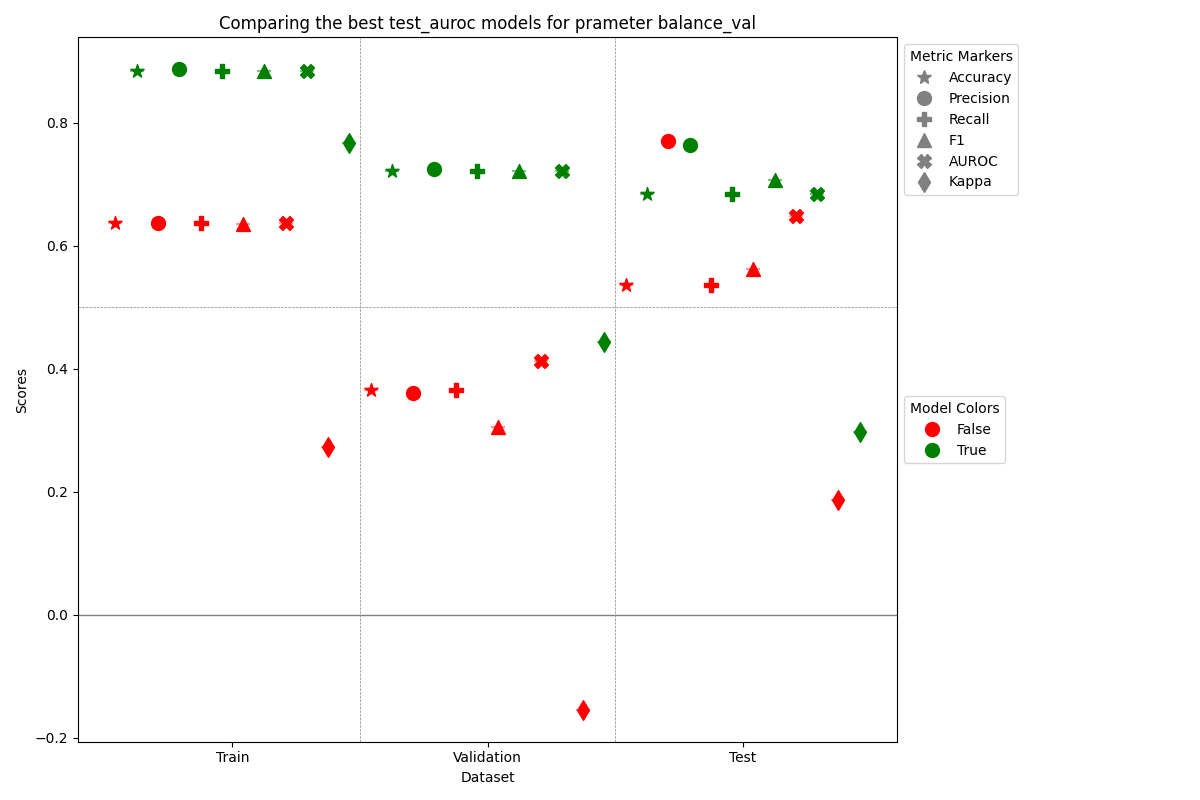
\includegraphics[width=400px]{Figures/results/balance_val/balance_val_test_auroc.png}
    \caption{The best models selected on the Test set AUROC score compared by the Balance Validation parameter.}
    \label{fig: balance_val_test_auroc}
\end{figure}

In \autoref{fig: balance_val_test_kappa}, the Balance Validation parameters are plotted for the models scoring the best on the Test set metric Kappa. This means that there are only two models plotted. The True value model scored better on all metrics on the Test set but worse on all others. The correspondence between the sets is much lower than the model selected through the Test AUROC score. The True valued model scores below chance on the Validation set for all metrics. The False valued model also has low correspondence between the sets. Both models' correspondence between the metrics is high, except for the False valued Kappa score.

\begin{figure}[H]
    \centering
    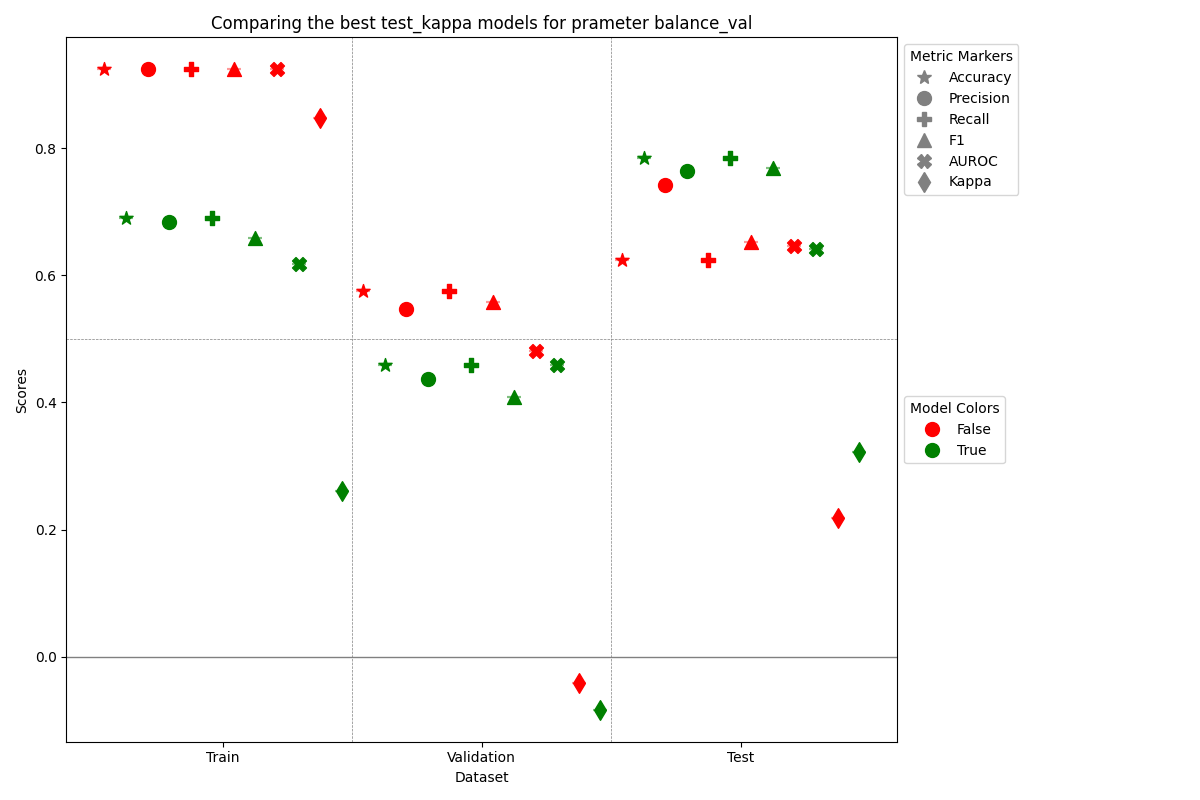
\includegraphics[width=400px]{Figures/results/balance_val/balance_val_test_kappa.png}
    \caption{The best models selected on the Test set Kappa score compared by the Balance Validation parameter.}
    \label{fig: balance_val_test_kappa}
\end{figure}

In \autoref{fig: balance_val_val_auroc}, the Balance Validation parameters are plotted for the models scoring the best on the Validation set metric AUROC. This means that there are only two models plotted. The True value model scored better on most metrics than the False valued model but scored much lower on the Test set than the others. The correspondence between the sets is lower than the model selected through the Test AUROC score. Unlike in \autoref{fig: balance_val_test_kappa}, the True valued models score above chance on all set metrics. The false valued model scores worse overall and is below or at least below the chance level for most of the metrics on the test set.


\begin{figure}[H]
    \centering
    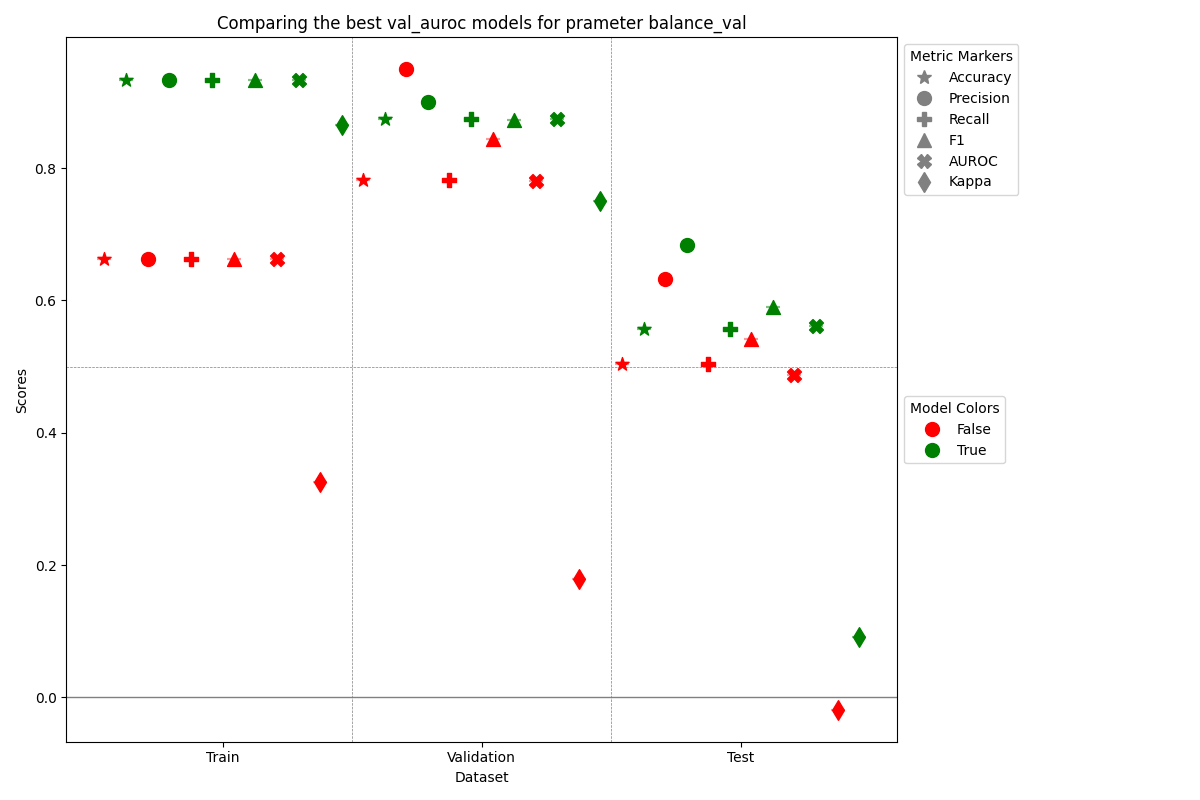
\includegraphics[width=400px]{Figures/results/balance_val/balance_val_val_auroc.png}
    \caption{The best models selected on the Validation set AUROC score compared by the Balance Validation parameter.}
    \label{fig: balance_val_val_auroc}
\end{figure}

In \autoref{fig: balance_val_val_kappa}, the Balance Validation parameters are plotted for the models scoring the best on the Validation set metric Kappa. This means that there are only two models plotted. The True value model scored better on all metrics on all sets than the False valued model. It seems to be the same model as in \autoref{fig: balance_val_val_auroc}. The False valued model has better correspondence between the sets than the False model in \autoref{fig: balance_val_val_auroc} but gets significantly lower scores overall. 


\begin{figure}[H]
    \centering
    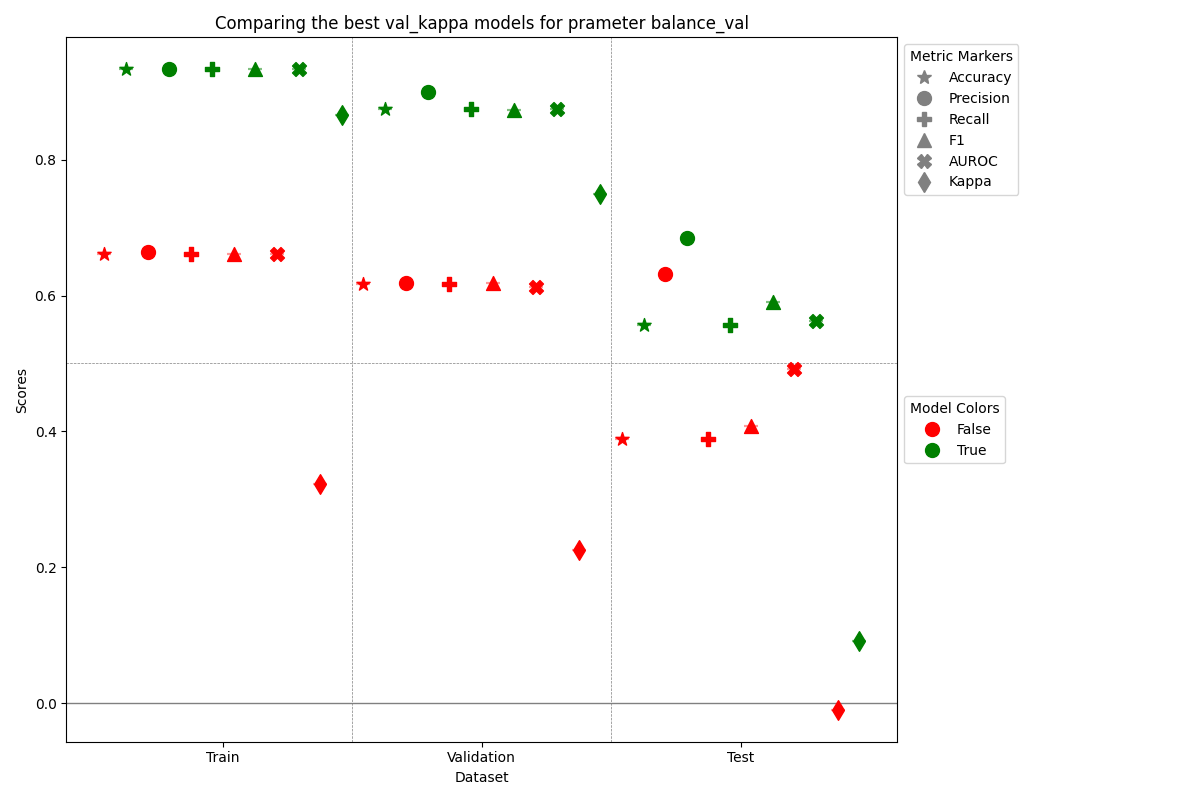
\includegraphics[width=400px]{Figures/results/balance_val/balance_val_val_kappa.png}
    \caption{The best models selected on the Validation set Kappa score compared by the Balance Validation parameter.}
    \label{fig: balance_val_val_kappa}
\end{figure}

\section{MEMD Data Augmentation}
\label{res_sec: memd_data_aug}
The MEMD Data Augmentation parameter is a boolean value used to turn off and on synthetic data generation. A True value signifies synthetic data generated using the MEMD method is added to the dataset, while a False value means no synthetic data is added. From the plots, it seems not using synthetic data is a bit better in the average, while in the best performing models, it's hard to tell if it seems the selection criteria play a more significant role for Test set scores.

In \autoref{fig: memd_data_augmentation_on}, the difference statistics between different MEMD Data Augmentation parameter values are compared on the three sets. On average (indicated by the marker), the False value scores better on the Training and Validation Sets but worse on the Test set for most metrics. The standard deviations (indicated by the vertical lines with short horizontal lines at the caps) seem larger on most metrics for the False value, especially on the Training set. The False parameter value appears to have the highest maximum values (topmost horizontal line) and the lowest minimum values (bottommost horizontal line) for all metrics in most sets.

\begin{figure}[H]
    \centering
    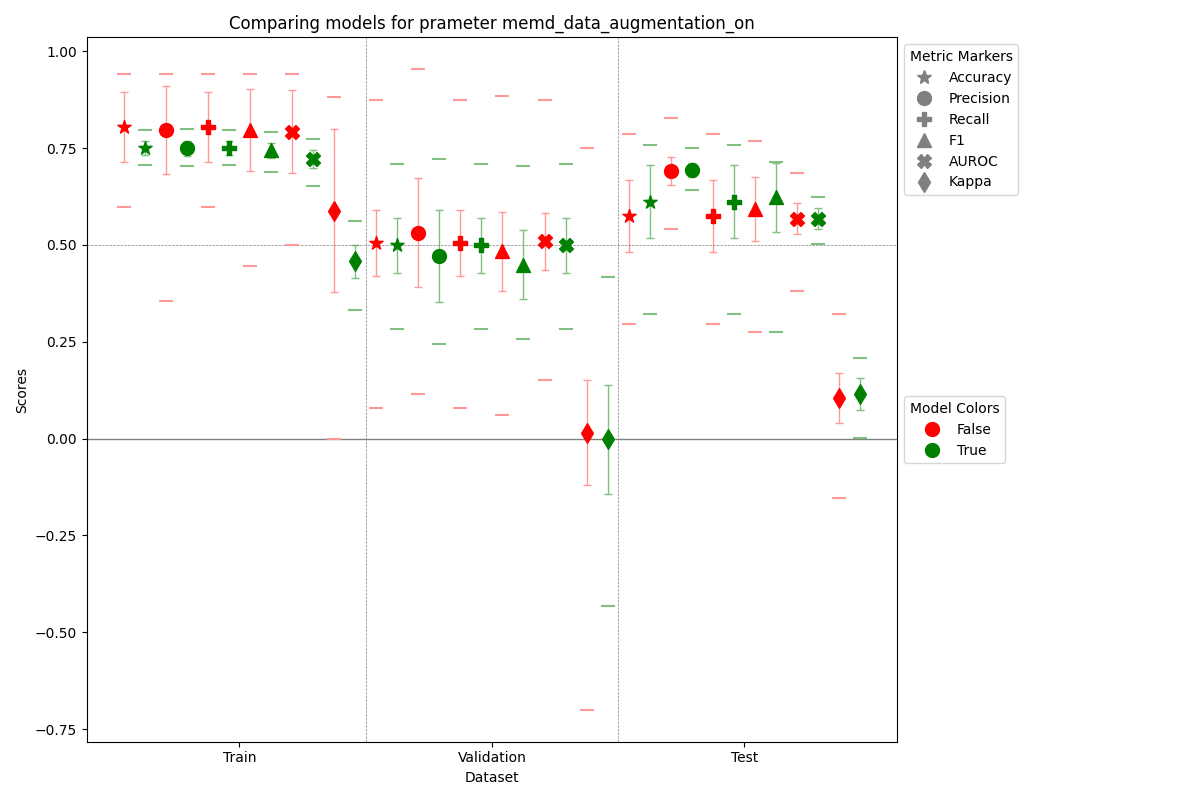
\includegraphics[width=400px]{Figures/results/memd_data_augmentation_on/memd_data_augmentation_on.png}
    \caption{All models compared by the MEMD Data Augmentation parameter, a True value signifies synthetic data generation using the MEMD method while a False value means no synthetic data.}
    \label{fig: memd_data_augmentation_on}
\end{figure}

In \autoref{fig: memd_data_augmentation_on_test_auroc}, the MEMD Data Augmentation parameters are plotted for the models scoring the best on the Test set metric AUROC. This means that there are only two models plotted. The False value model scored significantly better on all metrics on all sets. The correspondence between the sets is also high, with a low but consistent drop in scores from Training to Validation to Test.


\begin{figure}[H]
    \centering
    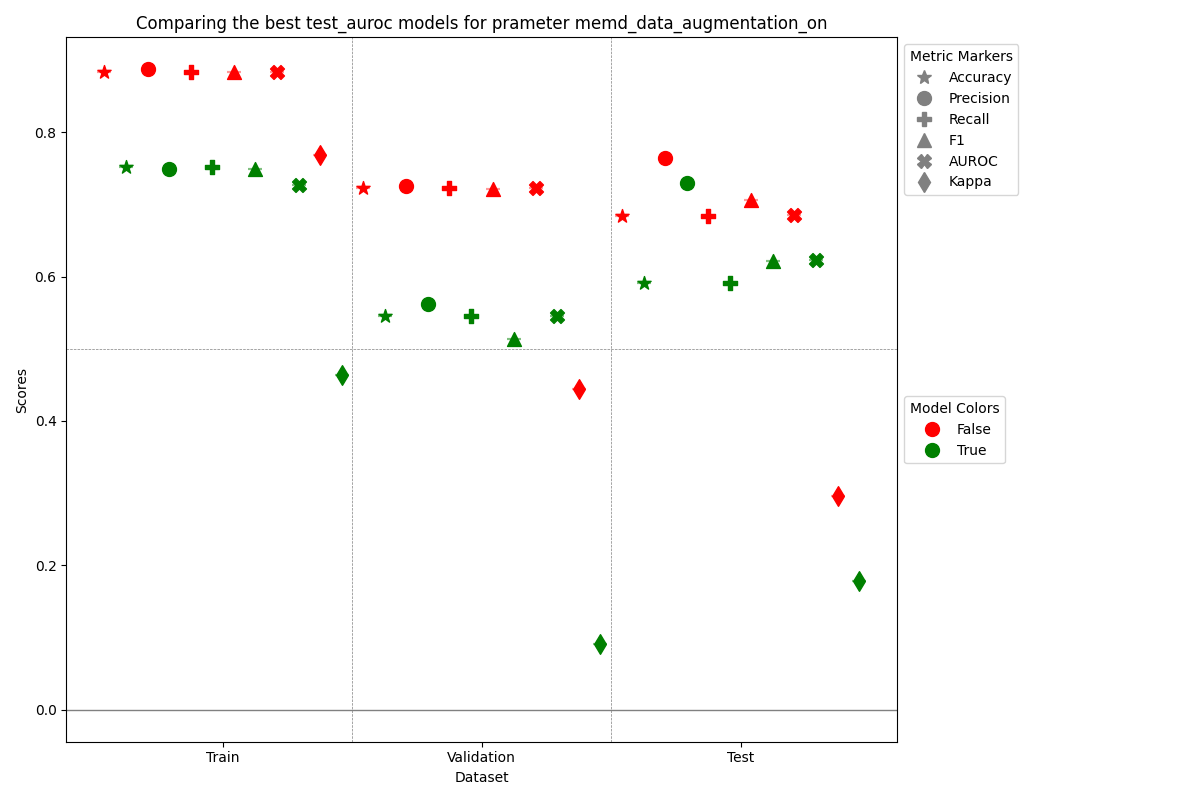
\includegraphics[width=400px]{Figures/results/memd_data_augmentation_on/memd_data_augmentation_on_test_auroc.png}
    \caption{The best models selected on the Test set AUROC score compared by the MEMD Data Augmentation parameter.}
    \label{fig: memd_data_augmentation_on_test_auroc}
\end{figure}

In \autoref{fig: memd_data_augmentation_on_test_kappa}, the MEMD Data Augmentation parameters are plotted for the best models scoring on the Test set metric Kappa. This means that there are only two models plotted. The False value model scored better on all metrics on the Test set but worse on all others. The correspondence between the sets is much lower than the model selected through the Test AUROC score. The False valued model scores below chance on the Validation set for all metrics. The True valued model also has low correspondence between the sets but is better than the False. The correspondence between the metrics is high for both models.

\begin{figure}[H]
    \centering
    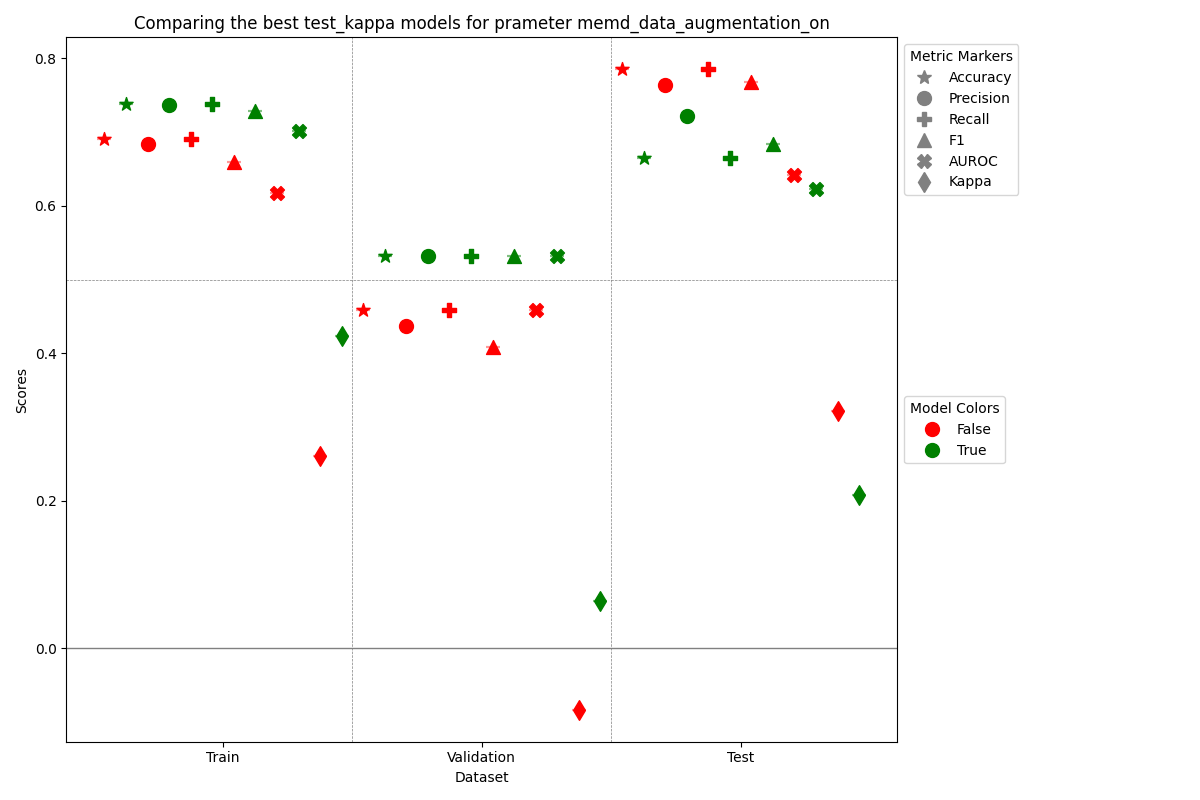
\includegraphics[width=400px]{Figures/results/memd_data_augmentation_on/memd_data_augmentation_on_test_kappa.png}
    \caption{The best models selected on the Test set Kappa score compared by the MEMD Data Augmentation parameter.}
    \label{fig: memd_data_augmentation_on_test_kappa}
\end{figure}

In \autoref{fig: memd_data_augmentation_on_val_auroc}, the MEMD Data Augmentation parameters are plotted for the models scoring the best on the Validation set metric AUROC. This means that there are only two models plotted. The False value model scored better on all metrics on the Training and Validation sets than the True valued model but scored significantly lower on the Test set than the other sets and worse than the True valued model. The correspondence between the sets is similar to the model selected through the Test AUROC score. Unlike in \autoref{fig: memd_data_augmentation_on_test_kappa}, the False valued models score above chance on all metrics on all sets. The True valued model scores better on the Test set and has higher correspondence between the sets.


\begin{figure}[H]
    \centering
    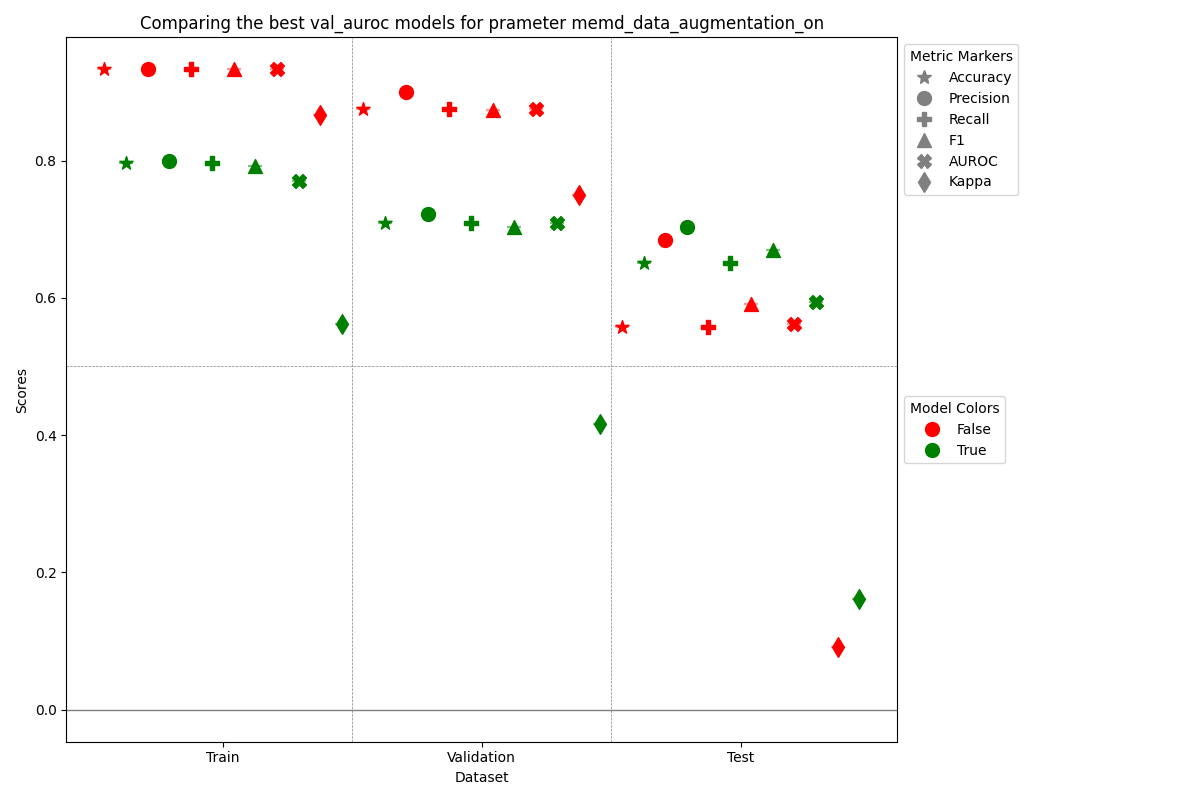
\includegraphics[width=400px]{Figures/results/memd_data_augmentation_on/memd_data_augmentation_on_val_auroc.png}
    \caption{The best models selected on the Validation set AUROC score compared by the MEMD Data Augmentation parameter.}
    \label{fig: memd_data_augmentation_on_val_auroc}
\end{figure}

In \autoref{fig: memd_data_augmentation_on_val_kappa}, the MEMD Data Augmentation parameters are plotted for the models scoring the best on the Validation set metric Kappa. It seems to be the same models selected as in \autoref{fig: memd_data_augmentation_on_val_auroc}, meaning both models were the best on both Kappa and AUROC on the Validation set.

\begin{figure}[H]
    \centering
    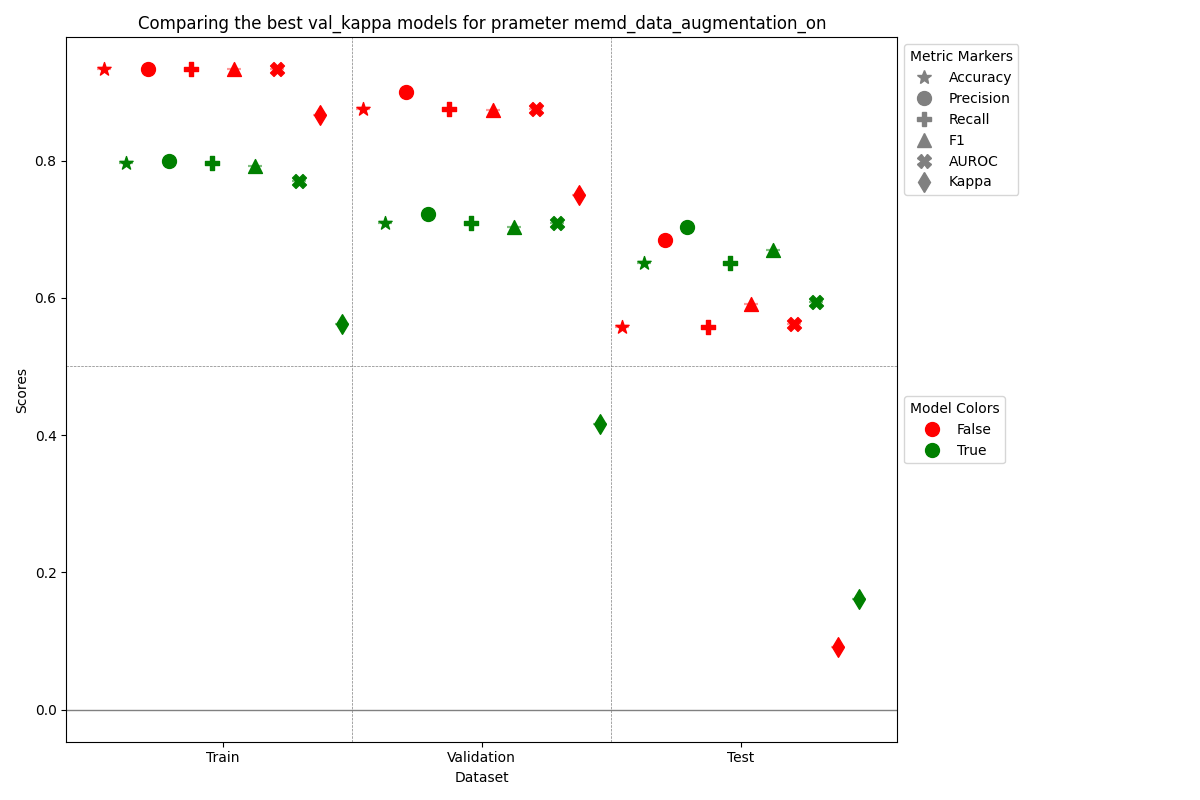
\includegraphics[width=400px]{Figures/results/memd_data_augmentation_on/memd_data_augmentation_on_val_kappa.png}
    \caption{The best models selected on the Validation set Kappa score compared by the MEMD Data Augmentation parameter.}
    \label{fig: memd_data_augmentation_on_val_kappa}
\end{figure}


\section{MEMD Ratio}
\label{res_sec: memd_ratio}
The MEMD Ratio parameter is a floating point value that signifies the ratio of the real data length to be generated synthetically using the MEMD method. A higher value means more synthetic data is generated and added to the Training set. A ratio of 1.0 means 50\% of the total training data is artificial, as explained in \autoref{subsec: augmentation_ratio}. It's essential to keep in mind that these values are only significant. 

As in \autoref{res_sec: balance_val} and \autoref{res_sec: memd_data_aug}, the correspondence between sets was best for the models scoring the best on the Test set using the metric AUROC. Also, like in \autoref{res_sec: memd_data_aug}, the same models scored the best on the metrics Kappa and AUROC on the Validation set. Due to this and the similarity of all parameter values, these plots have been left out.

In \autoref{fig: memd_ratio}, the difference statistics between different MEMD Ratio parameter values are compared on the three sets. It's hard to see the individual ratios due to the amount of metrics and parameter values plotted. However, this is chosen to showcase how similar these values are for all ratios. The data has been filtered to only use models with the MEMD Augmentation turned on to not skew the data since the Ratio parameter has no effect when turned off.

\begin{figure}[H]
    \centering
    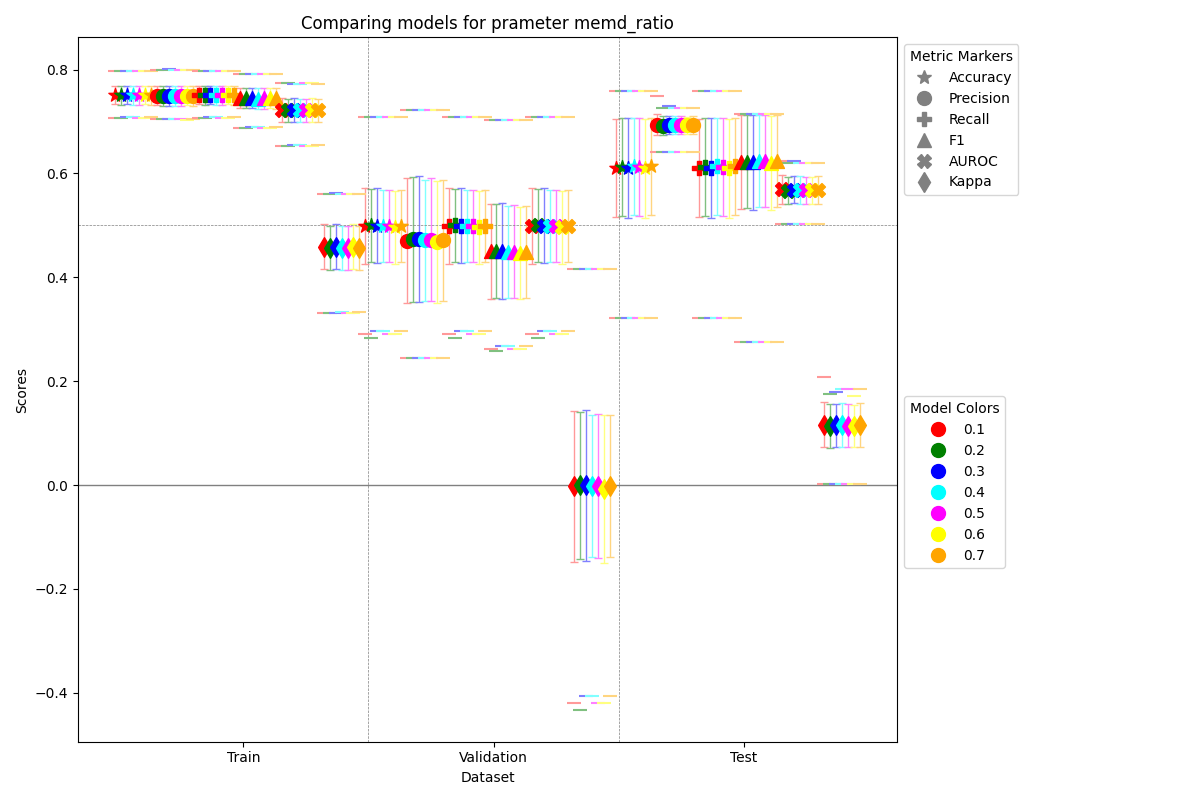
\includegraphics[width=400px]{Figures/results/memd_ratio/memd_ratio.png}
    \caption{All models compared by the MEMD Ratio parameter signifies the ratio of the real data length to be generated synthetically using the MEMD method. }
    \label{fig: memd_ratio}
\end{figure}
\begin{comment}
\begin{figure}[H]
    \centering
    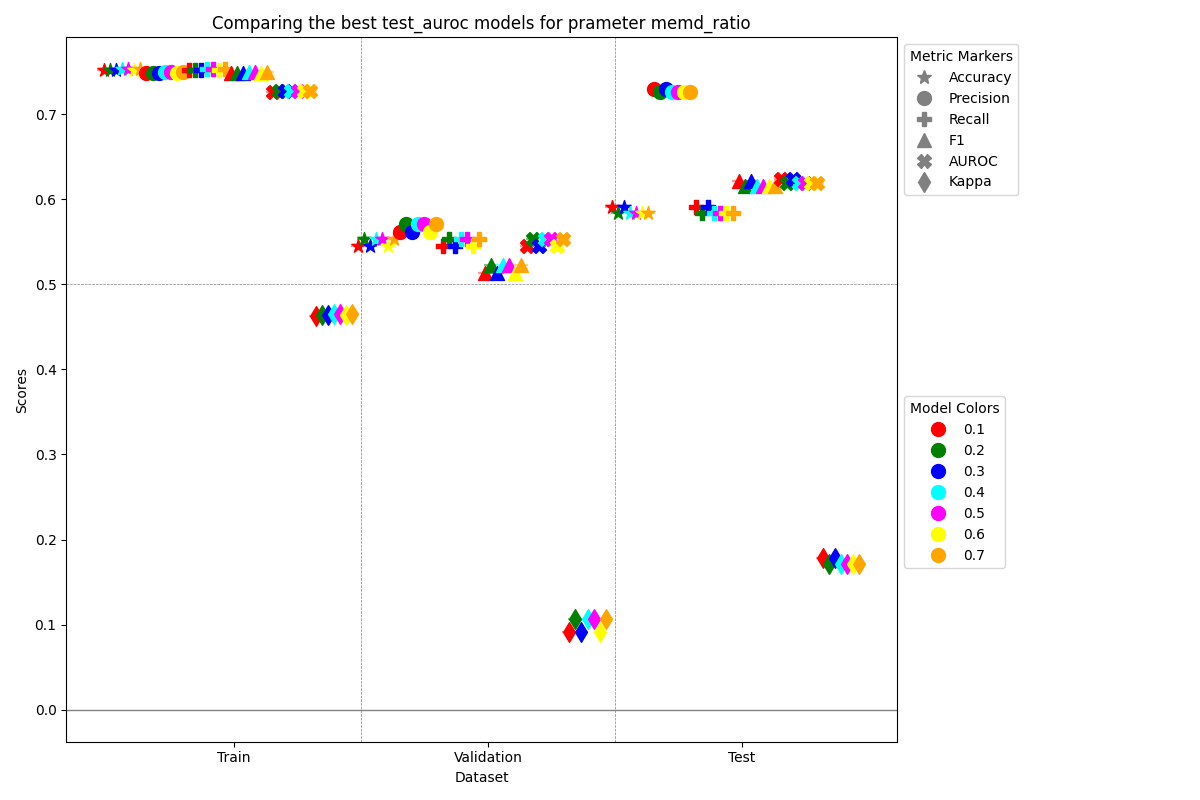
\includegraphics[width=400px]{Figures/results/memd_ratio/memd_ratio_test_auroc.png}
    \caption{The best models selected on the Test set AUROC score compared by the MEMD Ratio parameter.}
    \label{fig: memd_ratio_test_auroc}
\end{figure}


\begin{figure}[H]
    \centering
    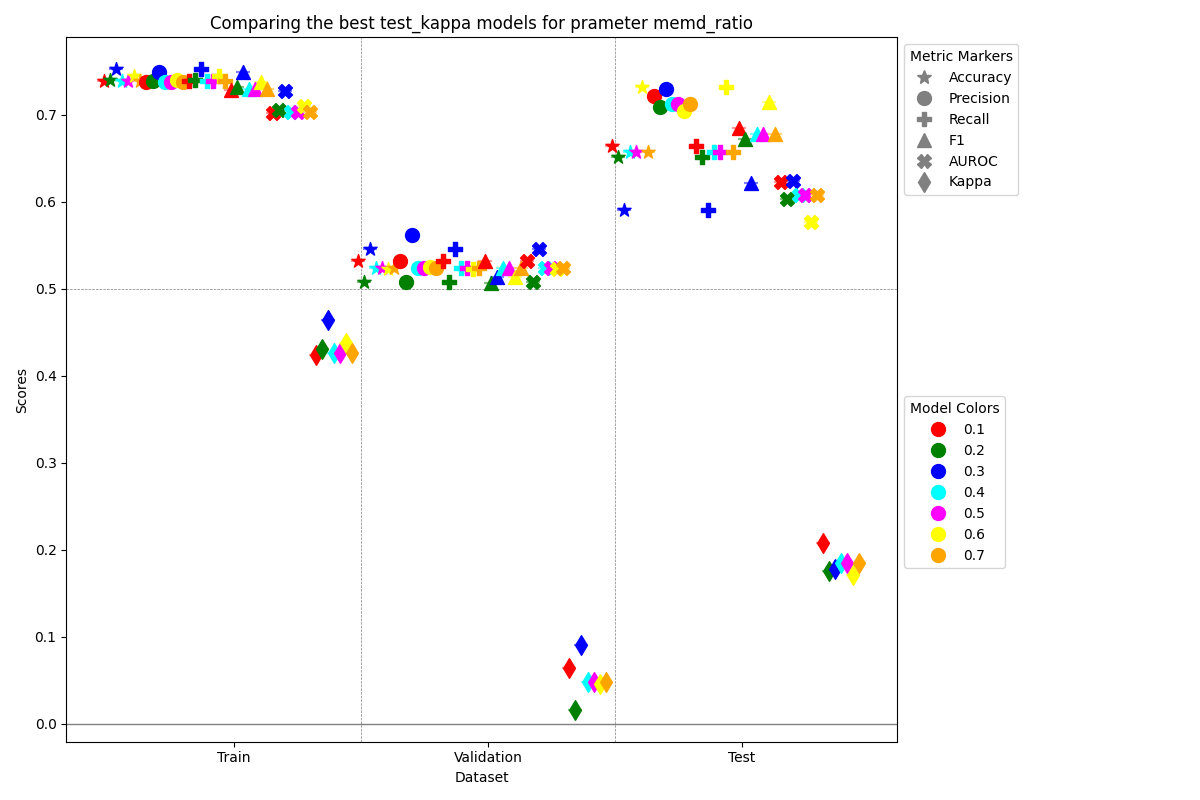
\includegraphics[width=400px]{Figures/results/memd_ratio/memd_ratio_test_kappa.png}
    \caption{The best models selected on the Test set Kappa score compared by the MEMD Ratio parameter.}
    \label{fig: memd_ratio_test_kappa}
\end{figure}

\begin{figure}[H]
    \centering
    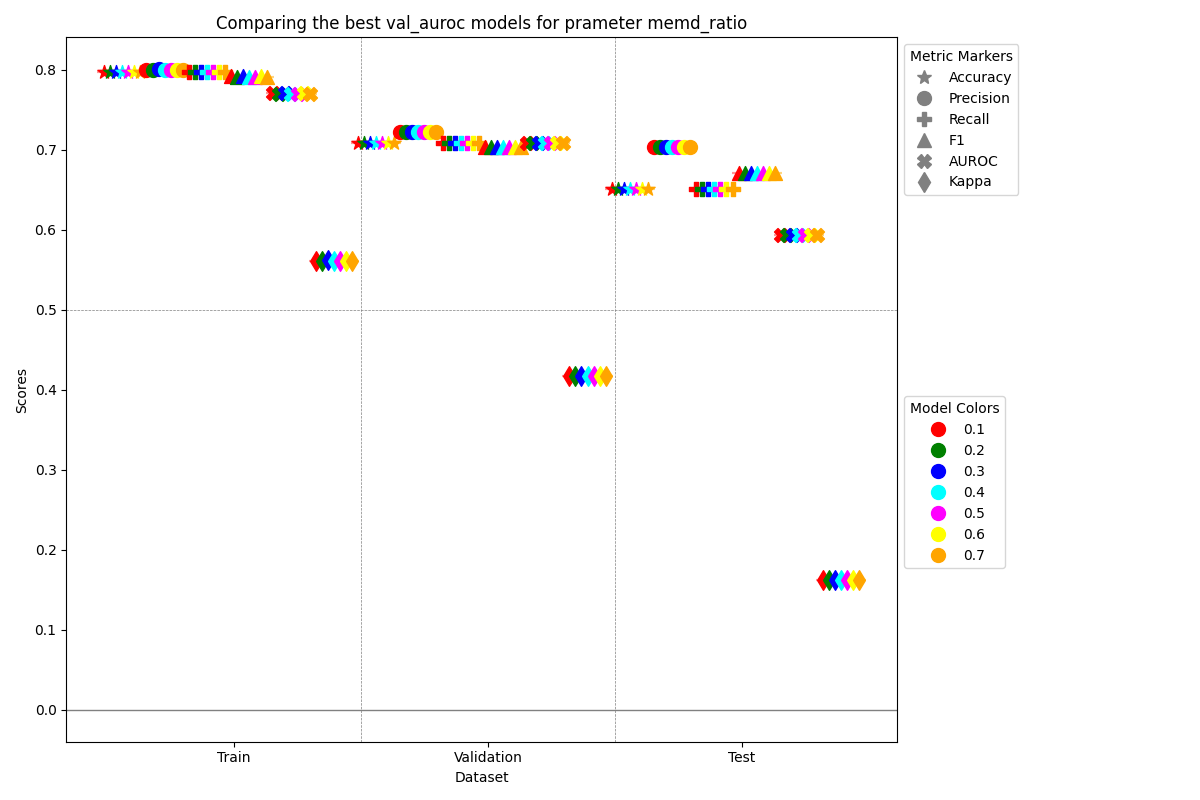
\includegraphics[width=400px]{Figures/results/memd_ratio/memd_ratio_val_auroc.png}
    \caption{The best models selected on the Validation set AUROC score compared by the MEMD Ratio parameter.}
    \label{fig: memd_ratio_val_auroc}
\end{figure}

\begin{figure}[H]
    \centering
    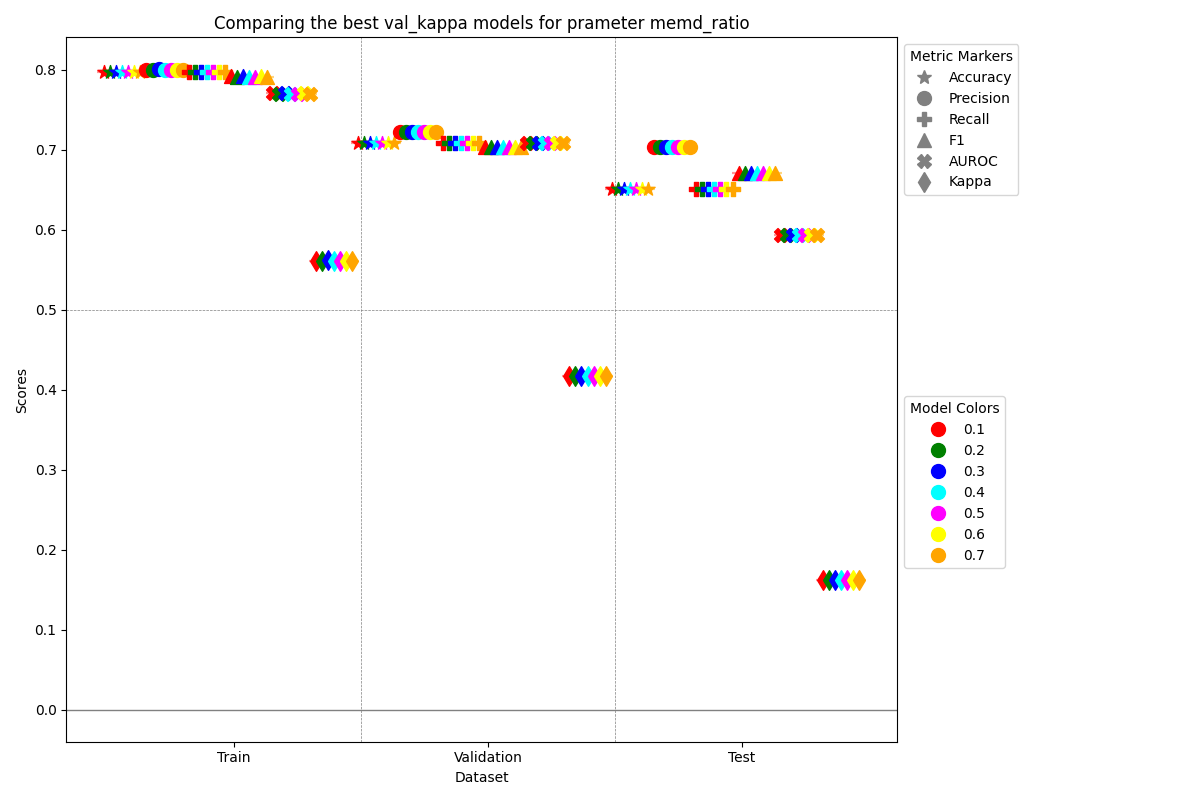
\includegraphics[width=400px]{Figures/results/memd_ratio/memd_ratio_val_kappa.png}
    \caption{The best models selected on the Validation set Kappa score compared by the MEMD Ratio parameter.}
    \label{fig: memd_ratio_val_kappa}
\end{figure}
\end{comment}


\section{IMF Cleaning}
The IMF Cleaning parameter is an integer or None value. A None value signifies no cleaning is done, and the raw signal is passed to the classifier. An integer value means the number of IMFs kept in the cleaned signal after sorting for importance, as explained in 
\autoref{subsec: img_selection}.

For similar reasons as in \autoref{res_sec: memd_ratio}, only the statistics plot and the models scoring the best on the Test set using the metric AUROC will be displayed in the results. 

In \autoref{fig: memd_ratio}, the difference statistics between different IMF Cleaning parameter values are compared on the three sets. Similarly to \autoref{res_sec: memd_ratio}, it is hard to see the individual values due to the number of metrics and parameter values plotted. However, this is chosen to showcase how similar these values are. 

\begin{figure}[H]
    \centering
    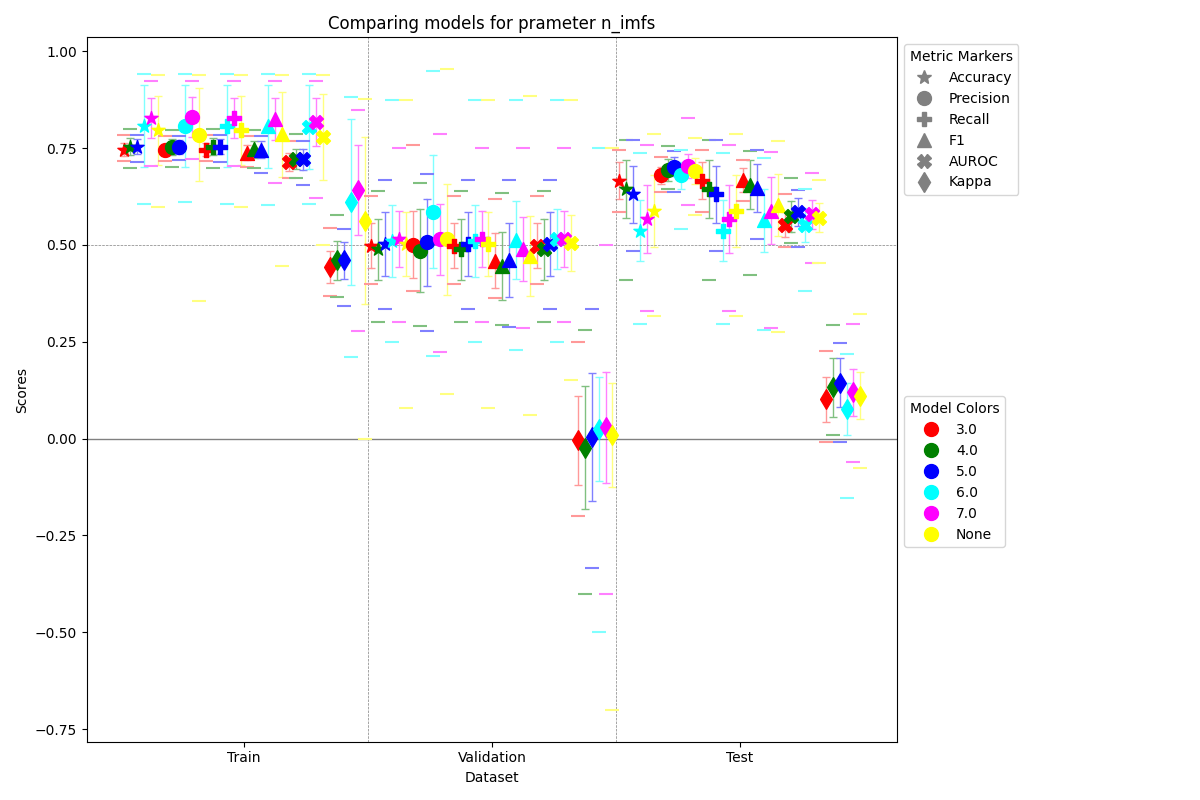
\includegraphics[width=400px]{Figures/results/n_imfs/n_imfs.png}
    \caption{All models compared by the IMF Cleaning parameter, a none value signifies no cleaning (raw signal) while a number means the number of IMFs kept in the cleaned signal after sorting for importance.}
    \label{fig: n_imfs}
\end{figure}


In \autoref{fig: memd_data_augmentation_on_test_auroc}, the IMF Cleaning parameters are plotted for the models scoring the best on the Test set metric AUROC. This means that there are only six different models plotted. It's clear that not cleaning scores worse on all sets. All the models seem to score more closely on the test set, with more significant discrepancies on the other sets. 


\begin{figure}[H]
    \centering
    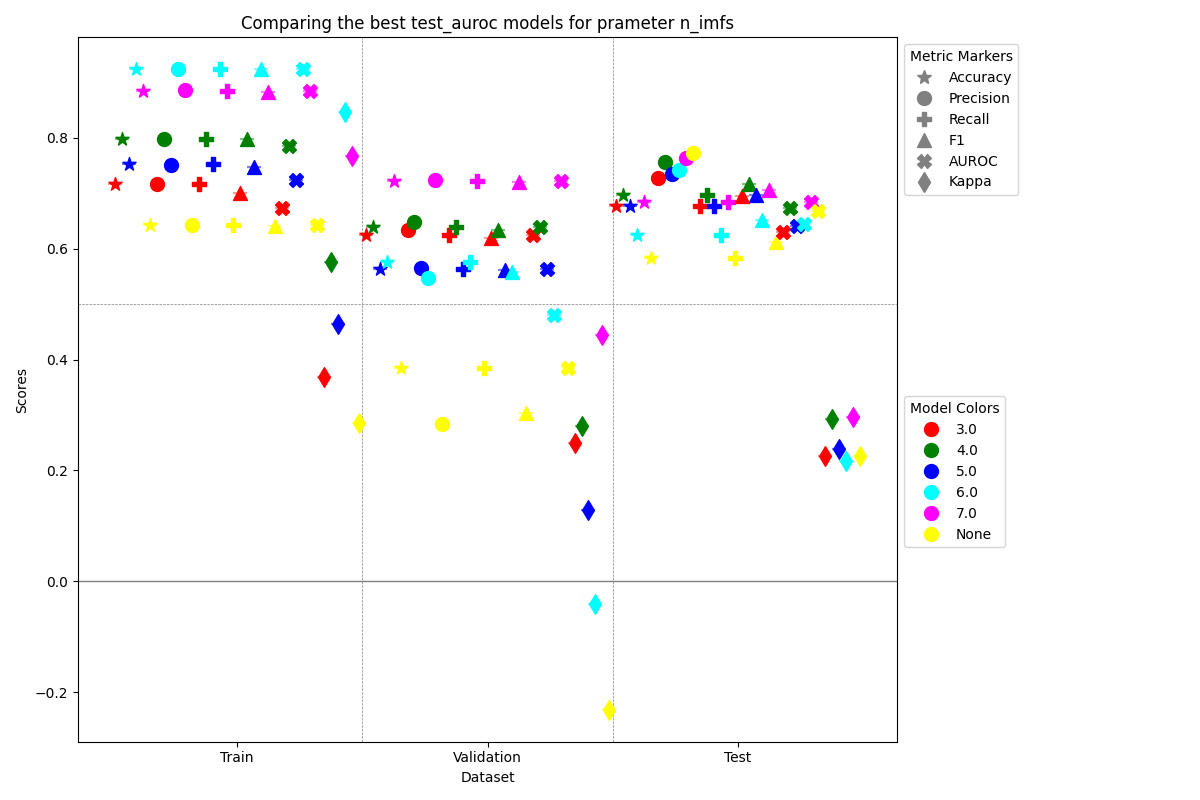
\includegraphics[width=400px]{Figures/results/n_imfs/n_imfs_test_auroc.png}
    \caption{The best models selected on the Test set AUROC score compared by the IMF Cleaning parameter.}
    \label{fig: n_imfs_test_auroc}
\end{figure}

\begin{comment}

\begin{figure}[H]
    \centering
    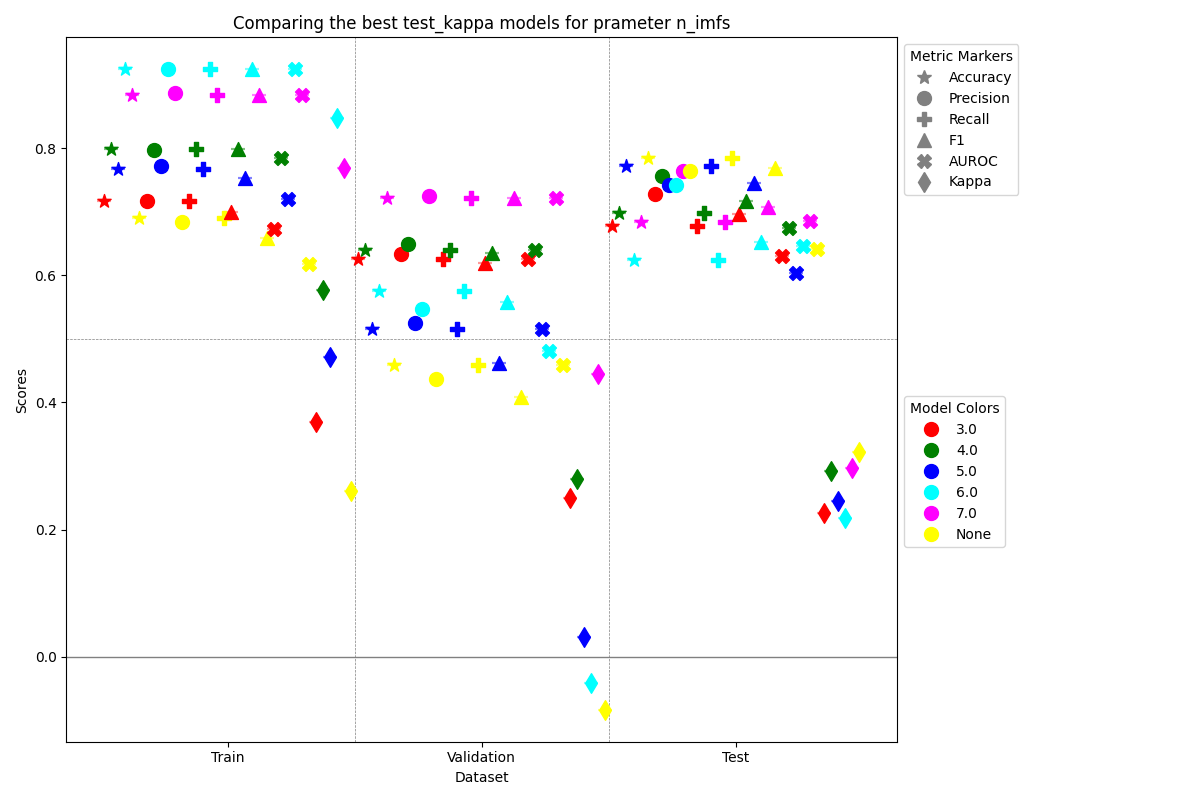
\includegraphics[width=400px]{Figures/results/n_imfs/n_imfs_test_kappa.png}
    \caption{The best models selected on the Test set Kappa score compared by the IMF cleaning parameter.}
    \label{fig: n_imfs_test_kappa}
\end{figure}

\begin{figure}[H]
    \centering
    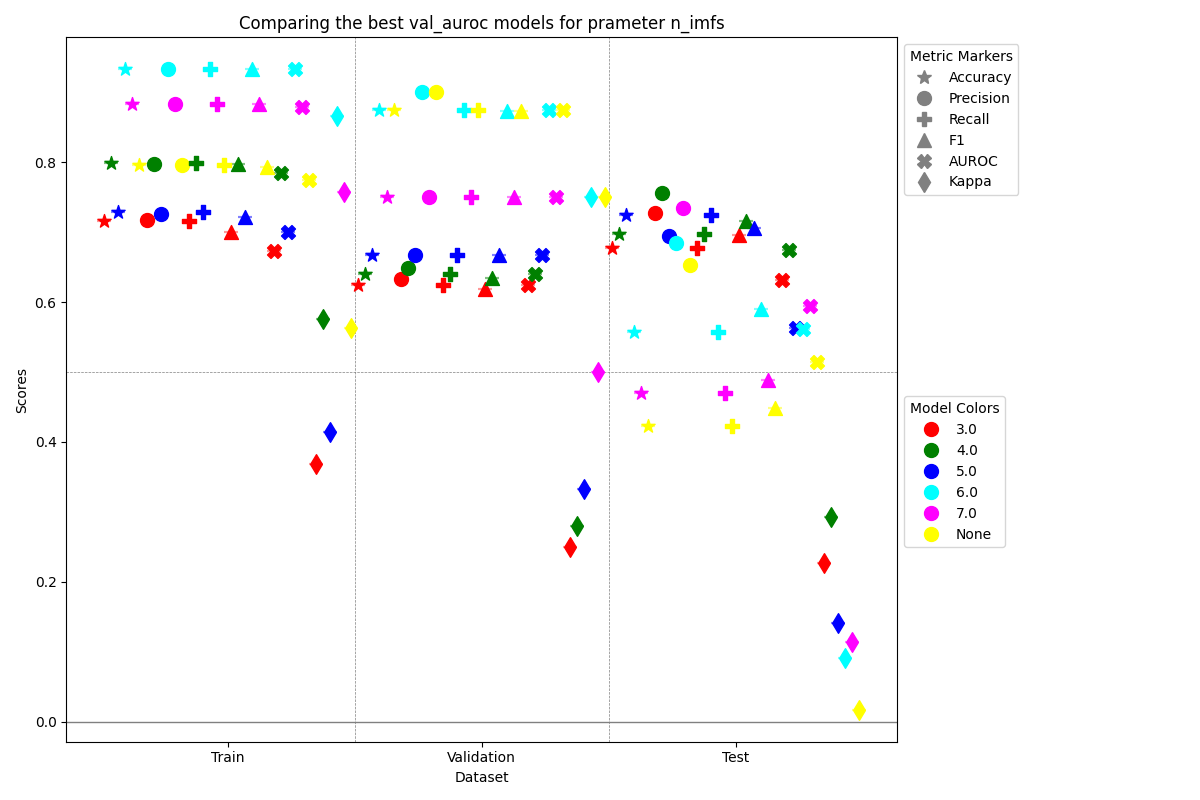
\includegraphics[width=400px]{Figures/results/n_imfs/n_imfs_val_auroc.png}
    \caption{The best models selected on the Validation set AUROC score compared by the IMF cleaning parameter.}
    \label{fig: n_imfs_val_auroc}
\end{figure}

\begin{figure}[H]
    \centering
    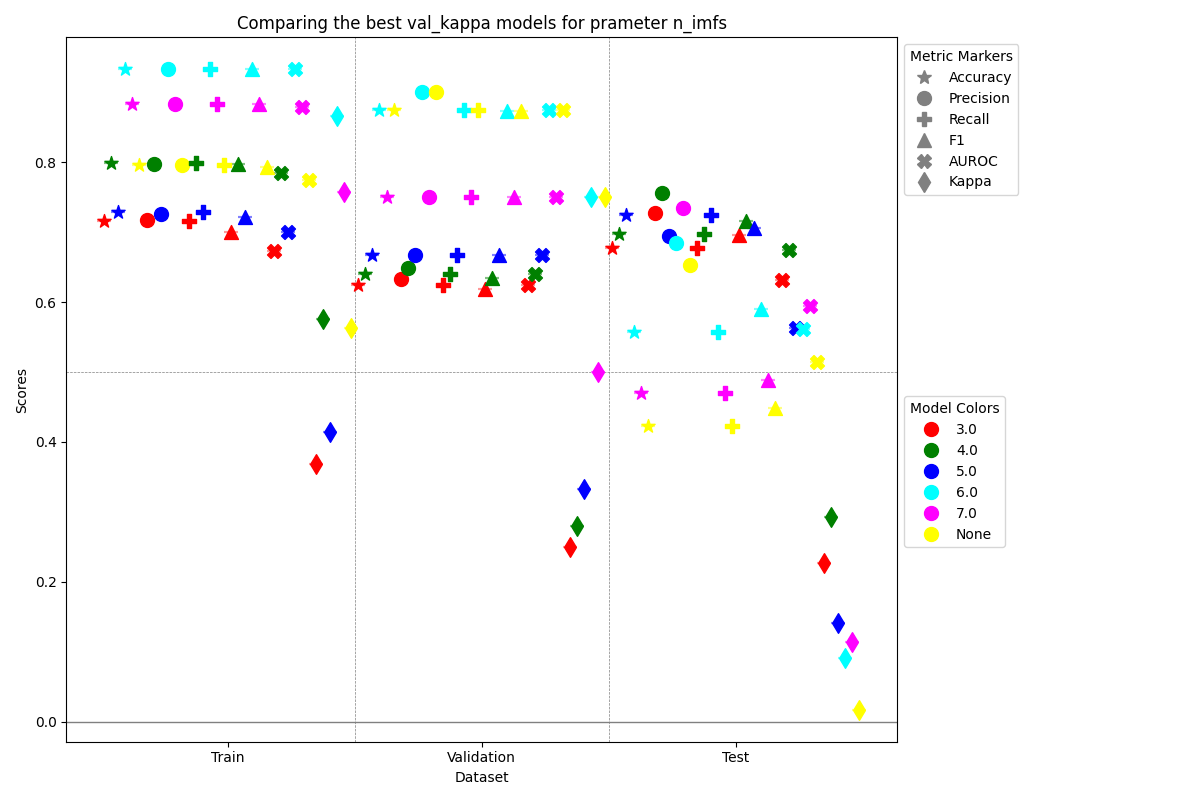
\includegraphics[width=400px]{Figures/results/n_imfs/n_imfs_val_kappa.png}
    \caption{The best models selected on the Validation set Kappa score compared by the IMF cleaning parameter.}
    \label{fig: n_imfs_val_kappa}
\end{figure}

\end{comment}


\section{Early Stopping Patience}
The Early Stopping Patience parameter is an integer value indicating how often the model can score worse than its best score on the Validation set for longer before the training loop is terminated. This is done to prevent overfitting to the training data. A higher value means the model can worsen for more epochs, potentially escaping local minima. A lower value potentially secures less overfitting.

For similar reasons as in \autoref{res_sec: memd_ratio}, only the statistics plot and the models scoring the best on the Test set using the metric Kappa will be displayed in the results. 

In \autoref{fig: patience}, the difference statistics between different Early Stopping Patience parameter values are compared on the three sets. Similarly to \autoref{res_sec: memd_ratio}, it is hard to see the individual values due to the number of metrics and parameter values plotted. However, this is chosen to showcase trends rather than personal values. It's clear from the Training set that higher Patience causes better results on all metrics. This does not seem to transfer to the other sets, where the relationship is less evident in both the average and extreme cases.


\begin{figure}[H]
    \centering
    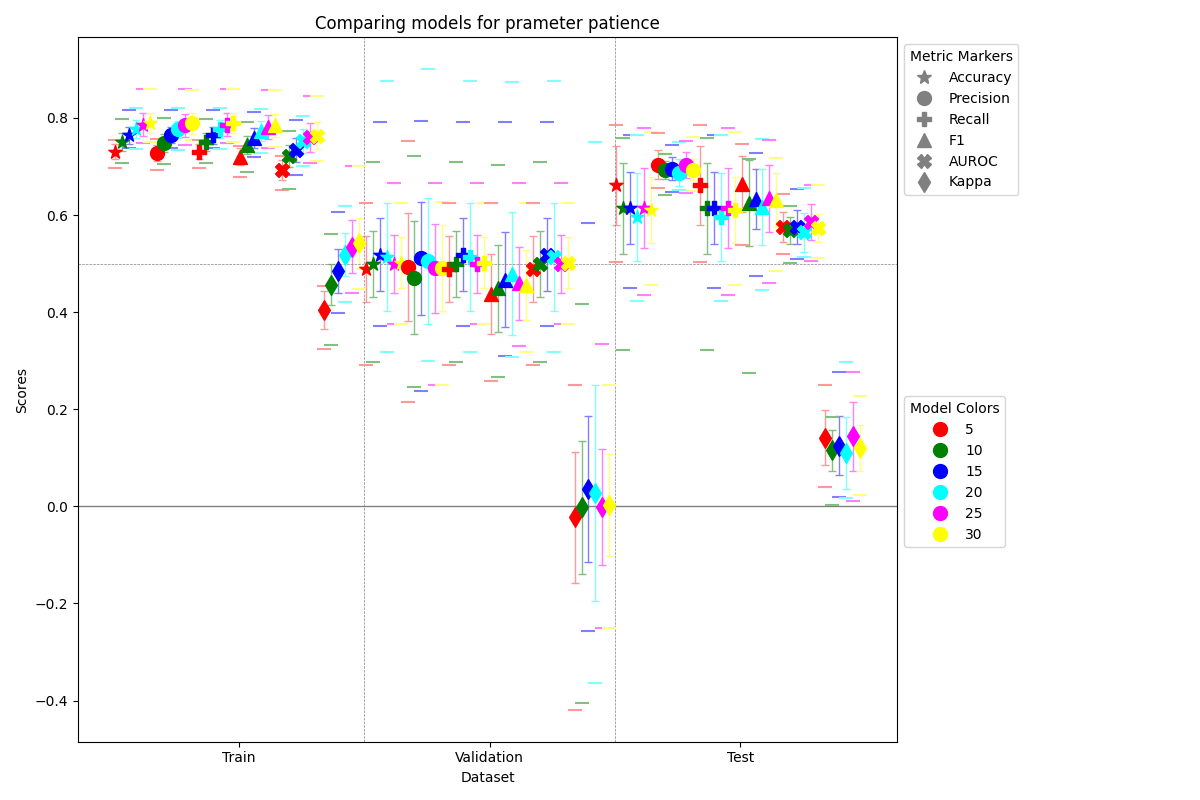
\includegraphics[width=400px]{Figures/results/patience/patience.png}
    \caption{All models compared by the Early Stopping Patience parameter, a higher value means the model can score worse than the best score on the Validation set so far for longer before the training loop is terminated.}
    \label{fig: patience}
\end{figure}


In \autoref{fig: patience_test_kappa}, the Early Stopping Patience parameters are plotted for the models scoring the best on the Test set metric Kappa. This means that there are only six different models plotted. Just like in the statistics case, it is clear from the Training set that higher Patience causes better results on all metrics. This does not seem to transfer well to the other sets. In the Test set, the relationship is weaker, but the parameter values from 15 to 25 seem to have the highest scores.

\begin{figure}[H]
    \centering
    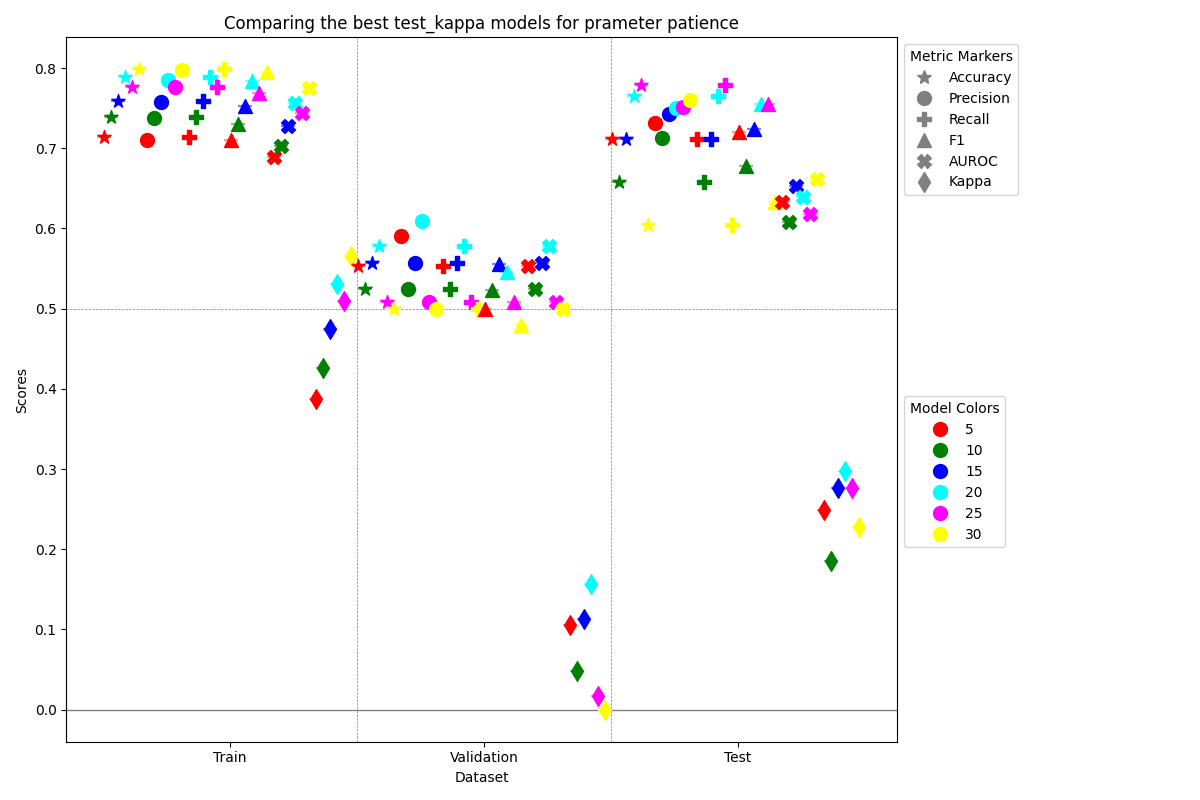
\includegraphics[width=400px]{Figures/results/patience/patience_test_kappa.png}
    \caption{The best models selected on the Test set Kappa score compared by the Early Stopping Patience parameter.}
    \label{fig: patience_test_kappa}
\end{figure}

\begin{comment}


\begin{figure}[H]
    \centering
    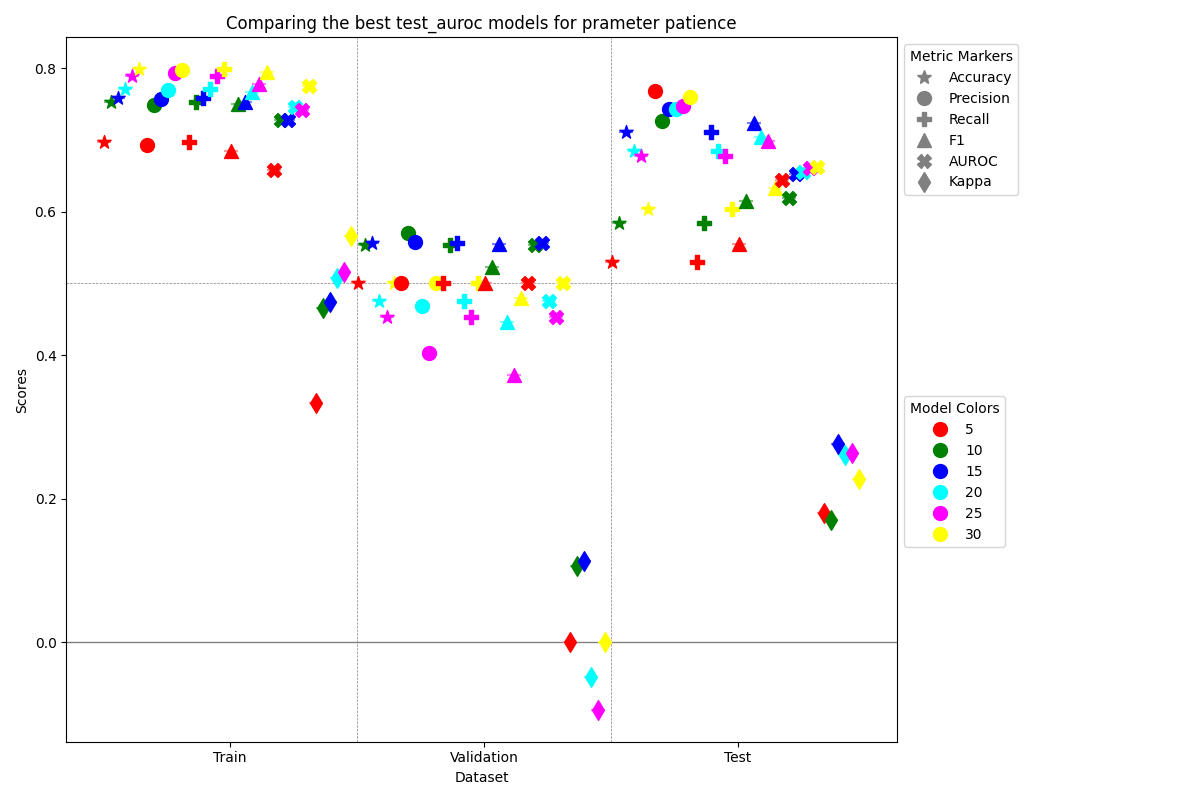
\includegraphics[width=400px]{Figures/results/patience/patience_test_auroc.png}
    \caption{The best models selected on the Test set AUROC score compared by the Early Stopping Patience parameter.}
    \label{fig: patience_test_auroc}
\end{figure}


\begin{figure}[H]
    \centering
    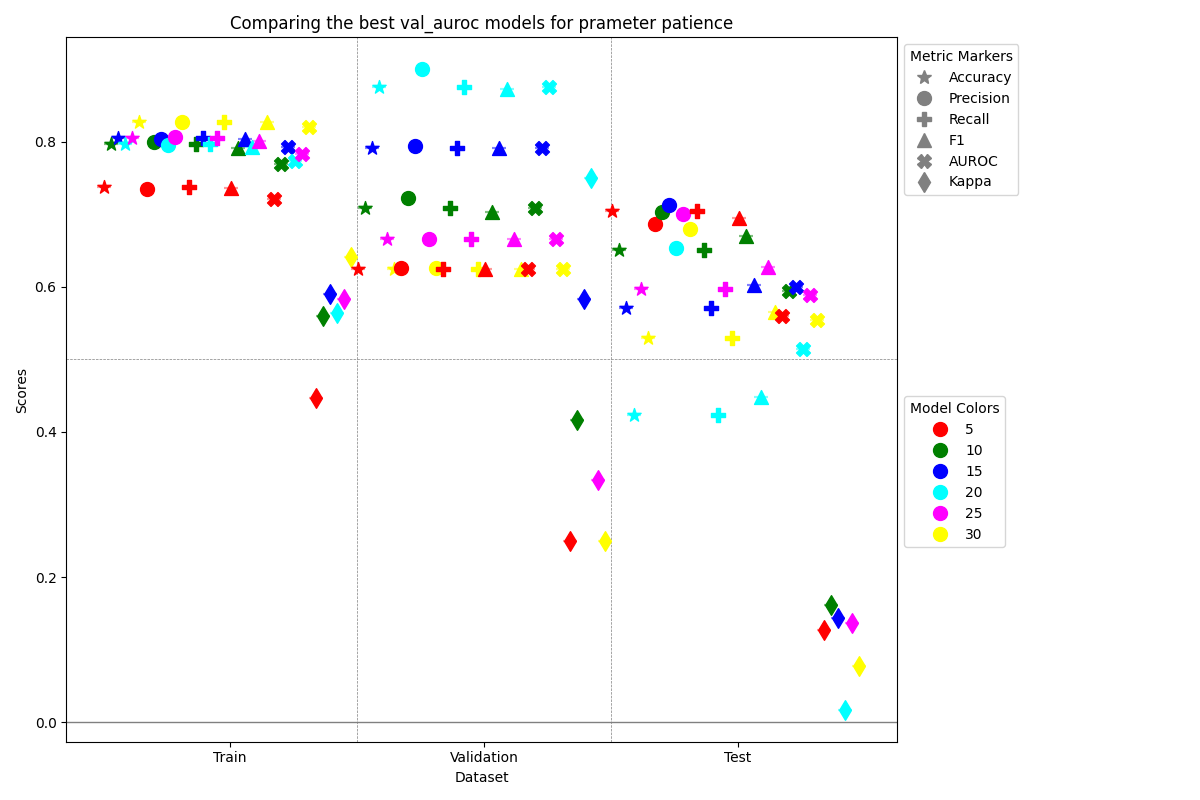
\includegraphics[width=400px]{Figures/results/patience/patience_val_auroc.png}
    \caption{The best models selected on the Validation set AUROC score compared by the Early Stopping Patience parameter.}
    \label{fig: patience_val_auroc}
\end{figure}

\begin{figure}[H]
    \centering
    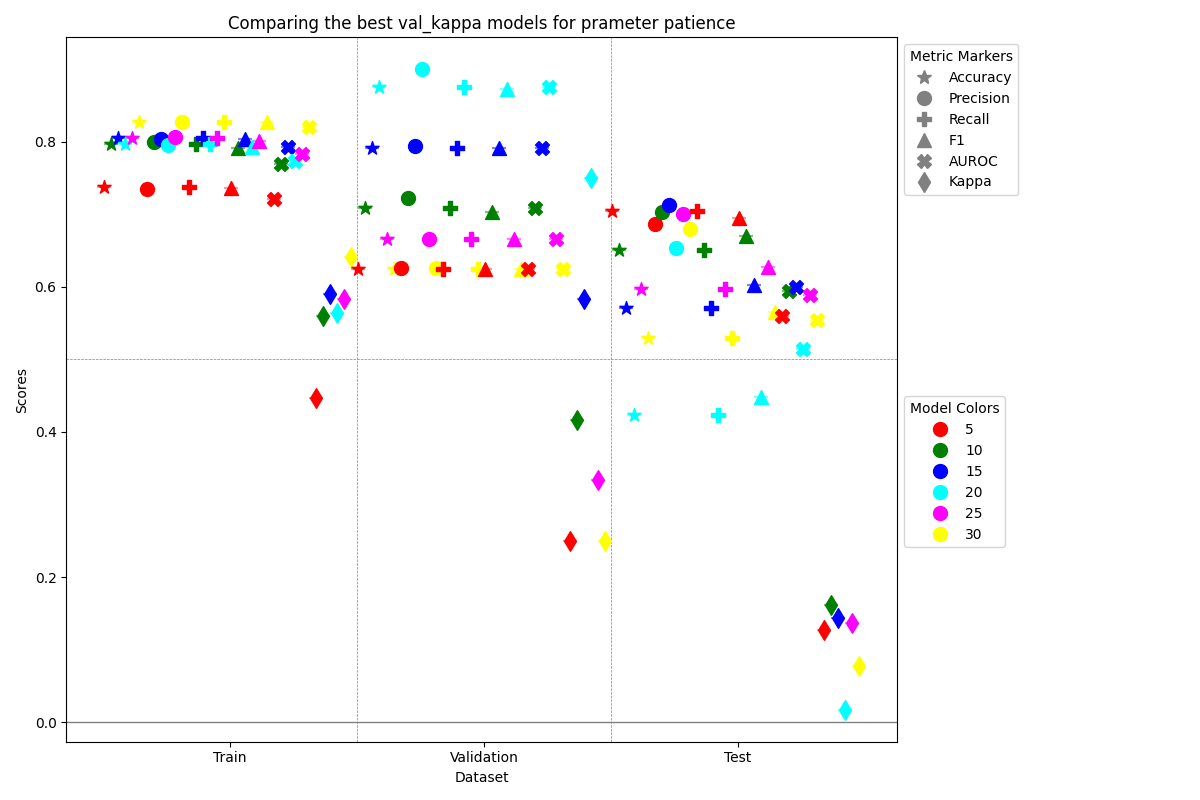
\includegraphics[width=400px]{Figures/results/patience/patience_val_kappa.png}
    \caption{The best models selected on the Validation set Kappa score compared by the Early Stopping Patience parameter.}
    \label{fig: patience_val_kappa}
\end{figure}

\end{comment}


\section{Regularization Techniques}
The Regularization Technique parameter is a string or None value parameter. The None value means no regularization is done on the data, while the string values of l1 or l2 choose the regularization method to regularize the data. The different techniques are explained in \autoref{subsec: regularization}.

In \autoref{fig: reg_type}, the difference statistics between different Regularization Technique parameter values are compared on the three sets. The L1 parameter value scores are lower or equal on all metrics and all average case sets. Looking at the maximum values, L1 also scores lower on most metrics. L2 and no regularization scores are very similar in the average case on all metrics, but in the extreme case, L2 scores are better for most metrics.

\begin{figure}[H]
    \centering
    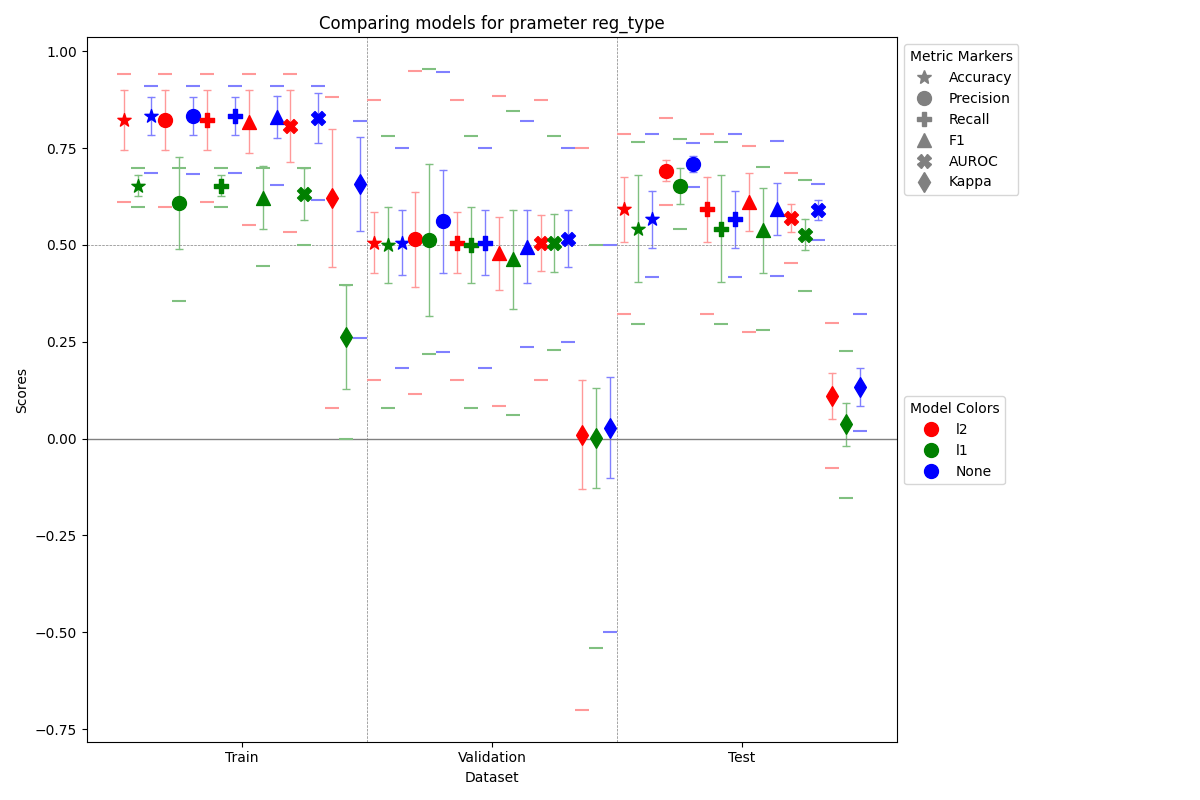
\includegraphics[width=400px]{Figures/results/reg_type/reg_type.png}
    \caption{All models compared by the Regularization Techniques parameter, the different methods are explained in \autoref{subsec: regularization}.}
    \label{fig: reg_type}
\end{figure}

In \autoref{fig: reg_type_test_auroc}, the Regularization Technique parameters are plotted for the models scoring the best on the Test set metric AUROC. This means that there are only three different models plotted. Just like in the statistics case, it is clear that L1 scores lower on most metrics. L2 has a good correspondence between sets, with the model scoring similarly on the Validation and Test sets. The no-regularization model varies from set to set and gets the best results for the test set.

\begin{figure}[H]
    \centering
    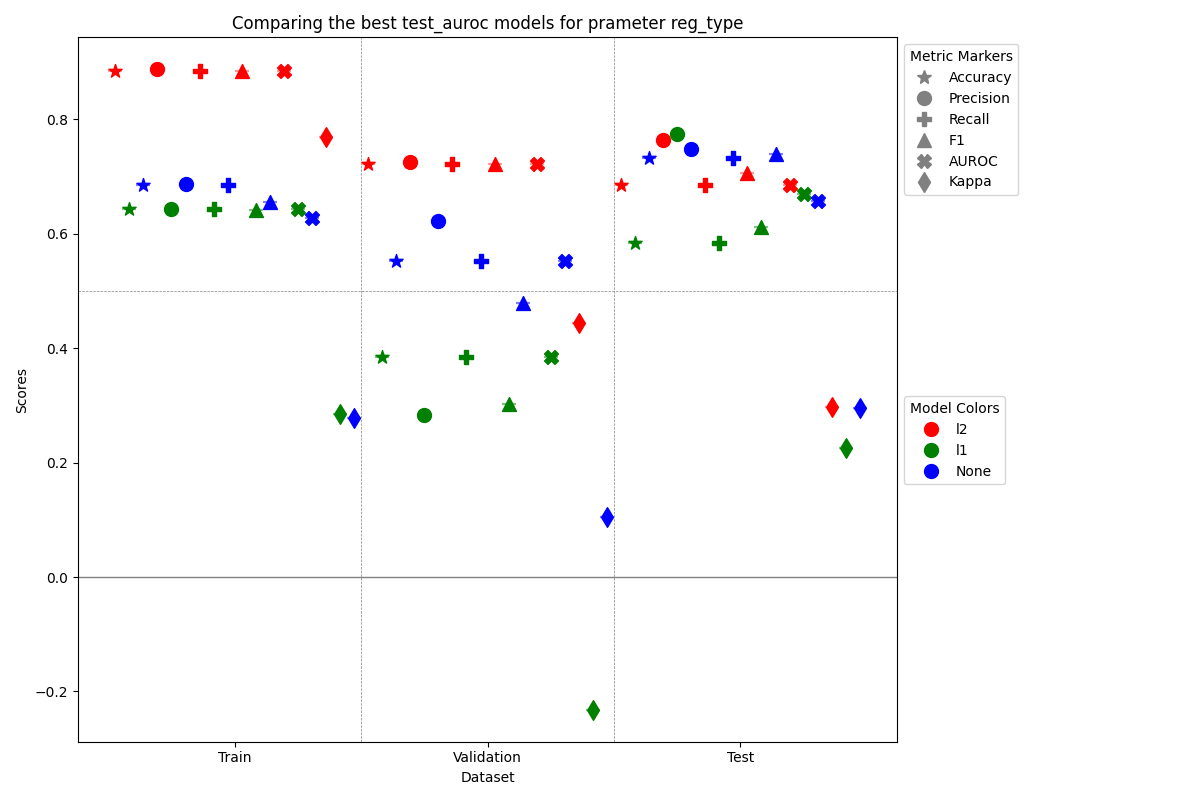
\includegraphics[width=400px]{Figures/results/reg_type/reg_type_test_auroc.png}
    \caption{The best models selected on the Test set AUROC score compared by the Regularization Techniques parameter.}
    \label{fig: reg_type_test_auroc}
\end{figure}

\begin{comment}

\begin{figure}[H]
    \centering
    \includegraphics[width=400px]{Figures/results/reg_type/reg_type_test_kappa.png}
    \caption{The best models selected on the Test set Kappa score compared by the Regularization Techniques parameter.}
    \label{fig: reg_type_test_kappa}
\end{figure}

\begin{figure}[H]
    \centering
    \includegraphics[width=400px]{Figures/results/reg_type/reg_type_val_auroc.png}
    \caption{The best models selected on the Validation set AUROC score compared by the Regularization Techniques parameter.}
    \label{fig: reg_type_val_auroc}
\end{figure}

\begin{figure}[H]
    \centering
    \includegraphics[width=400px]{Figures/results/reg_type/reg_type_val_kappa.png}
    \caption{The best models selected on the Validation set Kappa score compared by the Regularization Techniques parameter.}
    \label{fig: reg_type_val_kappa}
\end{figure}

\end{comment}






\section{Regularization Value}
This section compares different regularization values for the L2 method. A higher value means larger node values are punished harder, as explained in \autoref{subsec: regularization}. This tends to drive down the score on the training set as it overfits the training data less.

In \autoref{fig: reg_val}, the statistics of the difference between different Regularization Value parameter values are compared on the three sets. As expected, the scores on the Training set are inversely proportional to the Regularization Value. The average scores on the other sets are similar for all metrics, while the values of 0.05 and 0.1 score better in the extreme on both the Test and Validation sets.

\begin{figure}[H]
    \centering
    \includegraphics[width=400px]{Figures/results/reg_val/reg_val.png}
    \caption{All models compared by the Regularization Value parameter for the L2 method, a higher value means more regularization.}
    \label{fig: reg_val}
\end{figure}

In \autoref{fig: reg_val_test_auroc}, the Regularization Value parameters are plotted for the models scoring the best on the Test set metric AUROC. This means that there are only seven different models plotted. Just like in the statistics case, the scores on the training set align well with expectations. The 0.1 value scores best on most metrics in the Test set, while the 0.05 value has the best correspondence between the three sets while getting good scores.

\begin{figure}[H]
    \centering
    \includegraphics[width=400px]{Figures/results/reg_val/reg_val_test_auroc.png}
    \caption{The best models selected on the Test set AUROC score compared by the Regularization Value parameter.}
    \label{fig: reg_val_test_auroc}
\end{figure}


\begin{comment}

\begin{figure}[H]
    \centering
    \includegraphics[width=400px]{Figures/results/reg_val/reg_val_test_kappa.png}
    \caption{The best models selected on the Test set Kappa score compared by the Regularization Value parameter.}
    \label{fig: reg_val_test_kappa}
\end{figure}

\begin{figure}[H]
    \centering
    \includegraphics[width=400px]{Figures/results/reg_val/reg_val_val_auroc.png}
    \caption{The best models selected on the Validation set AUROC score compared by the Regularization Value parameter.}
    \label{fig: reg_val_val_auroc}
\end{figure}

\begin{figure}[H]
    \centering
    \includegraphics[width=400px]{Figures/results/reg_val/reg_val_val_kappa.png}
    \caption{The best models selected on the Validation set Kappa score compared by the Regularization Value parameter.}
    \label{fig: reg_val_val_kappa}
\end{figure}

\end{comment}


\section{Dropout Rate}
This section compares different dropout rate values. A higher Dropout Rate means more network nodes are turned off at offndom during training as explained in \autoref{subsec: regularization}. This tends to drive down the score on the training set as it overfits the training data less.

In \autoref{fig: dropout}, the difference statistics between different Dropout Rate parameter values are compared in \ three sets. As expected, the scores on the Training set are inversely proportional to the Dropout Rate. The average scores on the Test set seem to be proportional to the Dropout Rate value, while on the Validation set, most values score similarly. 

\begin{figure}[H]
    \centering
    \includegraphics[width=400px]{Figures/results/dropout/dropout.png}
    \caption{All models compared by the Dropout Rate parameter, a higher value means more dropout.}
    \label{fig: dropout}
\end{figure}

In \autoref{fig: dropout_test_auroc}, the Dropout Rate parameters are plotted for the models scoring the best on the Test set metric AUROC. This means that there are only nine different models plotted. Just like in the statistics case, the scores on the training set align well with expectations. The values 0.1 and 0.6 seem to score the highest on most metrics in the Test set, while 0.8 seems to have the most correspondence between scores across the different sets.


\begin{figure}[H]
    \centering
    \includegraphics[width=400px]{Figures/results/dropout/dropout_test_auroc.png}
    \caption{The best models selected on the Test set AUROC score compared by the Dropout Rate parameter.}
    \label{fig: dropout_test_auroc}
\end{figure}
\begin{comment}
\begin{figure}[H]
    \centering
    \includegraphics[width=400px]{Figures/results/dropout/dropout_test_kappa.png}
    \caption{The best models selected on the Test set Kappa score compared by the Dropout Rate parameter.}
    \label{fig: dropout_test_kappa}
\end{figure}

\begin{figure}[H]
    \centering
    \includegraphics[width=400px]{Figures/results/dropout/dropout_val_auroc.png}
    \caption{The best models selected on the Validation set AUROC score compared by the Dropout Rate parameter.}
    \label{fig: dropout_val_auroc}
\end{figure}

\begin{figure}[H]
    \centering
    \includegraphics[width=400px]{Figures/results/dropout/dropout_val_kappa.png}
    \caption{The best models selected on the Validation set Kappa score compared by the Dropout Rate parameter.}
    \label{fig: dropout_val_kappa}
\end{figure}

\end{comment}

\section{Dataset}
The dataset distribution is plotted in \autoref{fig: dataset_dist}. The subject with the lowest amount of total epochs is Subject 1, with 107 epochs. The subject with the highest amount of total epochs is Subject 25, with 208. 2/3 subjects have more than twice as many of one epoch type than the other. Of these 20 subjects, 16 have more than twice as much OT, while four have more than twice as much MW.
\begin{figure}[H]
    \centering
    \includegraphics[width=400px]{Figures/dataset_dist.png}
    \caption{Distribution of Epochs for every subject.}
    \label{fig: dataset_dist}
\end{figure}
%\section{Project thesis study data analysis}
%
\section{PANAS}

Here are some preliminary results from the PANAS questionnaire. The response level was coded as shown in \autoref{responselvl}, leading to a maximum average of 4, a minimum average of 0, and a mean of 2.


\begin{table}[htbp] % Table of resppnslevel
    \centering
    \caption{Response Level Categories}
    \begin{tabular}{|c|c|}
        \hline
        \textbf{Response Level} & \textbf{Numerical Value} \\
        \hline
        Very slightly or not at all & 0 \\
        A little & 1 \\
        Moderately & 2 \\
        Quite a bit & 3 \\
        Extremely & 4 \\
        \hline
    \end{tabular}
    \label{responselvl}
\end{table} %Respons level Table

\begin{figure}
    \centering
    \includegraphics[width=350px]{Figures/panas/avarages/Positive-Emotions.png}
    \caption{Plot of the Avarage Total Positive Emotions trend by practice in the PANAS questionnaire throughout the protocol.}
    \label{fig:positive_by_practice}
\end{figure} % Positive Avarage
\begin{figure}
    \centering
    \includegraphics[width=350px]{Figures/panas/avarages/Negative-Emotions.png}
    \caption{Plot of the Avarage Total Negative Emotions trend by practice in the PANAS questionnaire throughout the protocol.}
    \label{fig:negative_by_practice}
\end{figure} % Negative Avarage



\begin{figure}
    \centering
    \begin{minipage}{0.49\linewidth}
        \includegraphics[width=\linewidth]{Figures/panas/emotions/Active.png}
        \caption{Plot of the Active emotion trend by practice in the PANAS questionnaire throughout the protocol.}
        \label{fig:active_by_practice}
    \end{minipage}
    \hfill % Adds horizontal space between the figures
    \begin{minipage}{0.49\linewidth}
        \includegraphics[width=\linewidth]{Figures/panas/emotions/Afraid.png}
        \caption{Plot of the Afraid emotion trend by practice in the PANAS questionnaire throughout the protocol.}
        \label{fig:afraid_by_practice}
    \end{minipage}
\end{figure} % Active and Afraid plots

\begin{figure}
    \centering
    \begin{minipage}{0.49\linewidth}
        \includegraphics[width=\linewidth]{Figures/panas/emotions/Alert.png}
        \caption{Plot of the Alert emotion trend by practice in the PANAS questionnaire throughout the protocol.}
        \label{fig:alert_by_practice}
    \end{minipage}
    \hfill % Adds horizontal space between the figures
    \begin{minipage}{0.49\linewidth}
        \includegraphics[width=\linewidth]{Figures/panas/emotions/Ashamed.png}
        \caption{Plot of the Ashamed emotion trend by practice in the PANAS questionnaire throughout the protocol.}
        \label{fig:ashamed_by_practice}
    \end{minipage}
\end{figure} % Alert and Ashamed plots

\begin{figure}
    \centering
    \begin{minipage}{0.49\linewidth}
        \includegraphics[width=\linewidth]{Figures/panas/emotions/Attentive.png}
        \caption{Plot of the Attentive emotion trend by practice in the PANAS questionnaire throughout the protocol.}
        \label{fig:attentive_by_practice}
    \end{minipage}
    \hfill % Adds horizontal space between the figures
    \begin{minipage}{0.49\linewidth}
        \includegraphics[width=\linewidth]{Figures/panas/emotions/Determined.png}
        \caption{Plot of the Determined emotion trend by practice in the PANAS questionnaire throughout the protocol.}
        \label{fig:Determined_by_practice}
    \end{minipage}
\end{figure} % Attentive and Determined plots

\begin{figure}
    \centering
    \begin{minipage}{0.49\linewidth}
        \includegraphics[width=\linewidth]{Figures/panas/emotions/Distressed.png}
        \caption{Plot of the Distressed emotion trend by practice in the PANAS questionnaire throughout the protocol.}
        \label{fig:distressed_by_practice}
    \end{minipage}
    \hfill % Adds horizontal space between the figures
    \begin{minipage}{0.49\linewidth}
        \includegraphics[width=\linewidth]{Figures/panas/emotions/Enthusiastic.png}
        \caption{Plot of the Enthusiastic emotion trend by practice in the PANAS questionnaire throughout the protocol.}
        \label{fig:enthusiastic_by_practice}
    \end{minipage}
\end{figure} % Distressed and Enthusiastic plots

\begin{figure}
    \centering
    \begin{minipage}{0.49\linewidth}
        \includegraphics[width=\linewidth]{Figures/panas/emotions/Excited.png}
        \caption{Plot of the Excited emotion trend by practice in the PANAS questionnaire throughout the protocol.}
        \label{fig:excited_by_practice}
    \end{minipage}
    \hfill % Adds horizontal space between the figures
    \begin{minipage}{0.49\linewidth}
        \includegraphics[width=\linewidth]{Figures/panas/emotions/Guilty.png}
        \caption{Plot of the Guilty emotion trend by practice in the PANAS questionnaire throughout the protocol.}
        \label{fig:guilty_by_practice}
    \end{minipage}
\end{figure} % Excited and Guilty plots

\begin{figure}
    \centering
    \begin{minipage}{0.49\linewidth}
        \includegraphics[width=\linewidth]{Figures/panas/emotions/Hostile.png}
        \caption{Plot of the Hostile emotion trend by practice in the PANAS questionnaire throughout the protocol.}
        \label{fig:hostile_by_practice}
    \end{minipage}
    \hfill % Adds horizontal space between the figures
    \begin{minipage}{0.49\linewidth}
        \includegraphics[width=\linewidth]{Figures/panas/emotions/Inspired.png}
        \caption{Plot of the Inspired emotion trend by practice in the PANAS questionnaire throughout the protocol.}
        \label{fig:inspired_by_practice}
    \end{minipage}
\end{figure} % Hostile and Inspired plots

\begin{figure}
    \centering
    \begin{minipage}{0.49\linewidth}
        \includegraphics[width=\linewidth]{Figures/panas/emotions/Interested.png}
        \caption{Plot of the Interested emotion trend by practice in the PANAS questionnaire throughout the protocol.}
        \label{fig:interested_by_practice}
    \end{minipage}
    \hfill % Adds horizontal space between the figures
    \begin{minipage}{0.49\linewidth}
        \includegraphics[width=\linewidth]{Figures/panas/emotions/Irritable.png}
        \caption{Plot of the Irritable emotion trend by practice in the PANAS questionnaire throughout the protocol.}
        \label{fig:irritable_by_practice}
    \end{minipage}
\end{figure} % Interesed and Irritable plots

\begin{figure}
    \centering
    \begin{minipage}{0.49\linewidth}
        \includegraphics[width=\linewidth]{Figures/panas/emotions/Jittery.png}
        \caption{Plot of the Jittery emotion trend by practice in the PANAS questionnaire throughout the protocol.}
        \label{fig:jittery_by_practice}
    \end{minipage}
    \hfill % Adds horizontal space between the figures
    \begin{minipage}{0.49\linewidth}
        \includegraphics[width=\linewidth]{Figures/panas/emotions/Nervous.png}
        \caption{Plot of the Nervous emotion trend by practice in the PANAS questionnaire throughout the protocol.}
        \label{fig:nervous_by_practice}
    \end{minipage}
\end{figure} % Jittery and Nervous plots

\begin{figure}
    \centering
    \begin{minipage}{0.49\linewidth}
        \includegraphics[width=\linewidth]{Figures/panas/emotions/Proud.png}
        \caption{Plot of the Proud emotion trend by practice in the PANAS questionnaire throughout the protocol.}
        \label{fig:proud_by_practice}
    \end{minipage}
    \hfill % Adds horizontal space between the figures
    \begin{minipage}{0.49\linewidth}
        \includegraphics[width=\linewidth]{Figures/panas/emotions/Scared.png}
        \caption{Plot of the Scared emotion trend by practice in the PANAS questionnaire throughout the protocol.}
        \label{fig:scared_by_practice}
    \end{minipage}
\end{figure} % Proud and Scared plots

\begin{figure}
    \centering
    \begin{minipage}{0.49\linewidth}
        \includegraphics[width=\linewidth]{Figures/panas/emotions/Strong.png}
        \caption{Plot of the Strong emotion trend by practice in the PANAS questionnaire throughout the protocol.}
        \label{fig:strong_by_practice}
    \end{minipage}
    \hfill % Adds horizontal space between the figures
    \begin{minipage}{0.49\linewidth}
        \includegraphics[width=\linewidth]{Figures/panas/emotions/Upset.png}
        \caption{Plot of the Upset emotion trend by practice in the PANAS questionnaire throughout the protocol.}
        \label{fig:upset_by_practice}
    \end{minipage}
\end{figure} % Strong and Upset plots
%\section{State Anxiety Inventory}
%\section{Trait Anxiety Inventory}
%\section{PROMIS}
\cleardoublepage


\chapter{Discussion}
\section{Results discussion}
\subsection{Set Correlation}
The weaker positive relationships between test accuracy and both test kappa and test AUROC in \autoref{fig: test_corr_no_reg} provide insights into the model's performance and its use of the underlying data.

Since the Kappa measure accounts for agreement occurring by chance, a weak correlation with test accuracy might indicate that the dataset's inherent imbalance has not been fully accounted for or that the model performs differently across the classes. It suggests that while accuracy is high, the model might still be biased towards a particular class, i.e., on-task.
AUROC, on the other hand, measures the model's ability to distinguish between classes. A weak correlation with test accuracy could mean that the true positive and false positive rates do not vary proportionately with accuracy.

Thus, a high test accuracy combined with lower test kappa and test AUROC likely means that the model is overfitting the training data and not generalizing well to the unseen data. This implies that the accuracy metric alone is not sufficient to evaluate the model's performance and that the model has not reached its full potential.

In \autoref{fig: reg_type_scatter}, the different regularization techniques are compared in a scatterplot nature, which reveals some clear clusters between the Training and the other sets. Since the y=x line indicates a perfect correlation between the sets, a close fit to this line indicates no overfitting. Hence, even though the L1 metrics score substantially lower on the training set than the other metrics, it's, on average, less overfitted compared to Training and validation. This mainly falls away, though, when considering the test set. L1 mainly worsens the performance on the training set while only slightly improving it on the other sets. The model scoring the highest accuracy on both the Test and validation set used the L1 method; however, this might be more of a case of high variance as there is no clear trend of which method scores the best when comparing the Test and validation set.

The models scoring the highest and closest to the midline on the training validation plot get about an 85\% accuracy on both sets. In contrast, the best models closest to the midline for the validation test sets seem to be in the 65\% area for both sets. Most of these models use the L2 regularization technique.

Comparing the two Test set plots, it's evident that the model overfits the training set, as almost all points score below the midline, signifying higher Training than the test score. The same trend can be seen in the test validation plot, but to a lower degree, indicating that the models are less fitted to the validation set but still overfitted.

In \autoref{fig: reg_val_old}, different regularization values for the L2 method were tested to see which ones scored the best. As expected, higher regularization caused the score on the Training set to decrease, as less overfitting is expected. However...

\subsection{Balance Validation Set}
From the statistics plot \autoref{fig: balance_val}, it's clear that balancing the Validation set outperforms the models not balancing in the extreme, both on the Validation and Test set. This indicated that a balanced Validation set increases the generalization capabilities of the best models. Both parameters scored about the same on the training set, showing higher overfitting for the unbalanced models. 

Comparing \autoref{fig: balance_val_test_auroc} and \autoref{fig: balance_val_val_kappa}, it's clear that the selection metric and selection set greatly impact the model's general performance. Selection by AUROC tends to give a more balanced model with overall high performance. This can be seen in \autoref{fig: memd_data_augmentation_on_test_auroc} through \autoref{fig: memd_data_augmentation_on_val_kappa} as well. The models selected by AUROC also tend to slightly decrease performance from Training to Validation to Test, which is aligned with expectations as the models are expected to be better on seen data and data that performance is selected on. This trend indicated that it's a good selection criterion, that the selected model performs well, and that it is not a random chance. \cite{Jin2019PredictingMW} got an across task accuracy of 60\% which these models score well above. 
\subsection{MEMD Data Augmentation}
From \autoref{fig: memd_data_augmentation_on} through \autoref{fig: memd_data_augmentation_on_val_kappa}, it seems that not adding synthetic data to the dataset leads to the best performances overall. This is quite surprising as IMF-switched synthetic signals are expected to have close to real signal signatures, leading to more data with close to real values. This degradation of the results might be due to the swapping of IMFs or the capture of mind-wandering signatures in the interaction between IMFs, making the synthetic signals more confusing than helpful.
\subsection{MEMD Data Augmentation Ratio}
In \autoref{fig: memd_ratio}, it's clear that the ratios have next to no effect on the performances. This does not fit with the expectation since, from the results of adding synthetic data, we know that this decreases performance. Thus, a natural expectation is that more synthetic data would cause a worse performance, but this is not what is found. 
\subsection{IMF Cleaning}
In \autoref{fig: n_imfs}, all the metrics on the Training set are separated into two distinct groups in the average. The group of 3-5 IMFs and the group with 6,7 and no cleaning. The same trend is observed in accuracy, recall, and F1 on the test set. Looking at \autoref{fig: n_imfs_test_auroc}, the same split is evident, except for a surprisingly bad no-cleaning score. As the no-cleaning models score similarly to the 6 and 7 IMF models in the statistics plot, this might be a case of a particularly bad model scoring very high on the selection criteria and not an indication of more well-selected models. The low IMF models seem less overfitted in the Training set while scoring about the same on the Test set as the models with more IMFs.

\subsection{Early Stopping Patience}
In the statistics \autoref{fig: patience}, the expected result of a positive correlation between higher Patience and higher Training set scores on all metrics. As the Patience goes up, the model gets more overall runs through the training set, leading to overfitting, as can be seen by the average lower scores on the Test set for high patience models. However, as seen in the \autoref{fig: patience_test_kappa} setting, the Patience too low leads to models with too little Training with the medium, 15 to 25, patience models scoring the best on the Test set for the best models. The 20 and 25 patience models score the best for the overall metrics with accuracies of around 78\% and good scores on all other metrics in the Test set, giving higher confidence that the model has learned underlying features. 

\subsection{Regulariazation Techniques}
The statistics plot \autoref{fig: reg_type} is evident from the Training and Test set scores that the L1 is being outperformed. This could be due to too many nodes being effectively set to zero, as explained in \autoref{subsec: regularization}, or it could be that the regularization values tested were too high for the method. To answer this question, a specific L1 regularization value search could be performed in future project iterations.

In \autoref{fig: reg_type_test_auroc}, it's clear that the correlation between the Validation and Test set is highest for the L2 method and that L2 scores substantially higher on Training and Validation than the other methods. It's unsurprising that the L1 scores lower when looking at the statistics plot; however, it's clear from comparing the plots that the no-regularisation case performs well below its max and even average values on the training set. Thus, the model selection methodology of only using AUROC or Kappa on the Test set can lead to bad selections. Still, the L2 method seems to be a solid choice, but further exploration with better model selection is needed.

\subsection{Regularization Values for the L2 method}
As expected, the Training set scores are inversely proportional to the Regularization values, as seen in \autoref{fig: reg_val}. Looking at \autoref{fig: reg_val_test_auroc}, the same trend is evident in the Training set, with the middle values scoring the best on the Test set. In particular, 0.05 and 0.1 give good results for Test Kappa, with good scores on the other test metrics. 

\subsection{Dropout}
As expected, the Training set scores are inversely proportional to the Dropout values, as seen in \autoref{fig: dropout}. On the other hand, the Test set scores are proportional to the Dropout rate on most metrics and had little effect on others in the average case. In the no Droupout case of 0.0 in \autoref{fig: dropout_test_auroc}, a stark difference between Training and Test scores can be seen, indicating strong overfitting, while the 0.8 Dropout rate has a much closer fit between the two sets. Overall, the higher dropout rates seem to have much better correspondence between the different sets, while lower Dropout rates seem more varied. 0.2 seems like an outlier with much better correspondence than 0.0, 0.1, and 0.3, so it might not indicate a good parameter value but instead up to chance.

\section{Generalizability}
As explained in \autoref{sec: results_explanation}, all results were gathered using the General Model with the LOPO validation and test method. Hence, all validation and test set scores reflect model scores on EEG data from unseen participants, meaning the models can generalize well across subjects. This is surprising since EEG data is notoriously subject-specific. Hence, the models must have learned some underlying features shared between subjects. Thus, future expansion of the Transfer model with finetuning on individual subjects might lead to better individual prediction performance. 

The LOPO validation setup might also explain why some models score differently on the test and validation sets. One good way to reduce this discrepancy between the sets would be to opt for an LNPO method using N=2 or N=3 to reduce the variation.

\section{Dataset Critics}
In \autoref{fig: dataset_dist}, duplicated below for convenience, it's clear that the dataset is uneven in the aggregate volume of MW and OT and highly uneven within subjects. This leads to a few takeaways. 

One thing is that the data distribution seems highly unlikely for some subjects. As discussed in \autoref{sec: mind_wandering}, mind wandering is a common phenomenon, and the tasks performed by the subjects under the data collection were likely to induce mind wandering. This makes it unlikely that so many subjects have almost no mind wandering, and thus, many epochs might be mislabeled. Therefore, evaluating epochs as discussed in \autoref{subsec: study_design} could be valuable.

Another aspect is that since EEG signatures are highly individual, the high intra-subject imbalance might worsen any balancing methods. As individual nature worsens, the generalizability between subjects will worsen, and all balancing might need to be done within the subject. If this is the case, it could explain the poor performance of synthetic data found during testing, as all data has only been mixed within the class, not within subjects. However, this would mean that any over- or undersampling would duplicate or delete a lot more data than over- or undersampling in the aggregate, which has been tested. The same is true in the synthetic balancing case, as the synthetic data would be based on much smaller datasets. 
\begin{figure}[H]
    \centering
    \includegraphics[width=400px]{Figures/dataset_dist.png}
\end{figure}

\cleardoublepage

\chapter{Conclusions}

This thesis has laid the foundation for and explored the impact of various machine learning techniques and parameters on mind-wandering detection using EEG data. Through rigorous experimentation and analysis, it has provided insights into the complexities of EEG data processing and the generalization capabilities of neural networks across different subjects.

Regularization techniques such as L2 and dropout have been shown to be effective in mitigating overfitting. L2 demonstrates particularly robust performance in maintaining model generalization across training, validation, and test datasets. The choice of the regularization parameter played a critical role, with a moderate regularization level proving most effective in balancing model training and generalization.

The experiments with data augmentation, mainly using synthetic data through MEMD augmentation, highlighted the challenges of incorporating synthetic EEG data into training sets. While it was hypothesized that synthetic data would enhance model training by providing more samples, the results indicated otherwise, suggesting that synthetic data might introduce noise or irrelevant patterns that could confuse the learning algorithm. It is speculated that this is caused by data mixing between subjects.

Model performance metrics such as AUROC and Kappa provided a nuanced view of model effectiveness, underscoring the limitations of relying solely on accuracy for evaluating model performance, especially in unbalanced datasets. The application of different metrics revealed that while models could achieve high accuracy, their ability to discern between classes genuinely was not always satisfactory, indicating potential biases or overfitting to dominant classes.

Furthermore, deploying different dropout rates and early stopping techniques underscored the importance of carefully tuned hyperparameters in achieving optimal model performance. These techniques helped fine-tune the models to avoid overfitting while allowing adequate training.

The study also highlighted the significance of dataset characteristics, particularly the balance and distribution of data. The skewed distribution of mind-wandering episodes across subjects suggested potential mislabeling or inherent biases in the dataset, which could impact the training and performance of machine learning models. This calls for a more refined approach to data collection and preprocessing to ensure the reliability and validity of training datasets in EEG-based studies.

In conclusion, this thesis advances our understanding of the practical challenges in using machine learning for EEG data analysis and sets the groundwork for future research. It opens avenues for further exploration into more sophisticated data augmentation techniques, deeper analysis of regularization impacts, and the development of more robust models sensitive to the nuances of EEG data and the phenomenon of mind-wandering. Future studies could also explore the potential of transfer learning and fine-tuning models on individual subjects to enhance prediction accuracy and personalize mind-wandering detection systems, ultimately leading to more effective and user-tailored applications in real-world scenarios.
\cleardoublepage

\chapter{Future Work}
This chapter outlines possible improvements and extensions for the project, providing a foundation for future research and development. It aims to guide students and researchers interested in advancing the current project.

\section{Code Structure}
The existing codebase is well-structured with clearly defined modules such as config, IDUN pipeline, and main. Additionally, the folder hierarchy is logically organized. However, the src folder has grown considerably large and somewhat disorganized. Specifically, files like neural\_net\_utils.py have become excessively large and would benefit from being divided into multiple, more concise files to enhance readability and maintainability.

\subsection{Enhanced Plotting Capabilities}
The plotting code, originally developed in Jupyter Notebook, predates the creation of the model\_performance.csv file and thus does not utilize this common file for all model runs. Some plotting using the csv file has been implemented, but the capabilities are rather basic and should be improved. Future improvements should integrate this file, implementing functionalities for cleaning it, such as removing models lacking comprehensive metrics and adding additional plotting variations. This enhancement will streamline the process and make the plotting code more efficient. The current plotting code addresses complex comparison tasks, like identifying models with similar performance characteristics, and is a useful reference. Utilizing the Pandas library to handle the CSV data is recommended, as it will simplify data manipulation. Since visualizing model performance is crucial for understanding and improving the model, expanding these capabilities is essential.

\section{Label Validation Pipeline}
An area identified for future work is the development of a label validation pipeline. The dataset used in this thesis has raised some doubts regarding the validity of the epoch labels, particularly because the tasks performed by each subject were designed to induce mind wandering. Yet, it has resulted in data skewed towards 'on-task' performance, which seems improbable. For instance, one participant's data showed 100\% 'on-task' epochs, which is highly unlikely.

Two main approaches are proposed to address this issue. The first, simpler approach is implementing an exclusion paradigm, which removes participant epochs based on configuration or job parameter settings. The second, more involved approach involves creating a comprehensive validation pipeline. This would involve generating Event-Related Potentials (ERPs) for all epochs to visually verify whether they align with the labeled mental states against criteria derived from studies such as \cite{Rodriguez-Larios2020} and \cite{DelormeEEGMeditationStudy}. This additional labeling would then be stored for future runs and used to remove or relabel bad epochs.

\section{Extending the Models}
Although the transfer model has been developed, it has not undergone as extensive testing and application as the general model. Given the subject-specific nature of EEG data, transfer learning, particularly fine-tuning on the target subject, is expected to perform better. This approach will be especially beneficial if a substantial amount of data is collected from a single subject, which future students continuing the project could explore by doing testing on themselves.

The general model could also be further tuned; however, without additional data or new methods for increasing performance, the current version will unlikely be tuned to score substantially higher.

\section{Further parameter tuning}
Though many parameters have been explored it is likely that further optimization is possible. The L1 regularization method was not fully explored for optimal regularization values in this thesis and stands as a possible improvement. 

Also most parameters were explored with fixed values for all other parameters to figure out the individual contributions from the different parameter values possible within that parameter. This however leads to all synergetic effects between different parameters being lost, and as such continuing the search for optimal parameter combinations from smaller subsets of only the best possible values for every parameter is a adviced next step for finalizing the parameter tuning.

\section{Improvement in Model Selection}
The model selections in this thesis have mostly been based on the metrics AUROC and Kappa on the Test set. This was chosen as AUROC seemed to have the best overall correlation with other metrics, and  Kappa taking the dataset imbalance into account making it more informative. Howver, though this was a good choice given the time constraints some models picked using this method stilled scored very poorly on other metrics proving that this method can lead to picking a model overfitted to the specific metric. Hence creating a method for improved model selection is smart. This should be based on looking at scores on all metrics from all sets, while weighing different sets and metrics differently depending on their overall performance correlation. A rule of thumb used in this thesis has been that a slight negative slope from Training to Validation to Test is a good indication of a well adjusted model, since its expected that models perform better on seen data.

\section{Dataset Expansion}
More data is a common requirement in machine learning applications, particularly for data-intensive tasks such as EEG data classification.

\subsection{Creating a New Dataset}
One potential expansion involves creating a new dataset to replace or supplement the current one. This could be achieved by following protocols detailed in the theoretical portion of this thesis in \autoref{subsec: study_design} and would greatly benefit from an established validation pipeline. Implementing the Sustained Attention to Response Task (SART) with retrospective questionnaires and self-classification is recommended for reliable data collection.

\subsection{Verification Using Munk Dataset}
The \href{https://openneuro.org/datasets/ds001787/versions/1.0.3}{Munk dataset} contains EEG data from expert meditators, who typically have a profound understanding of their internal states. Utilizing this dataset could serve as a robust control to test the generalizability of the classifier developed in this project.

\subsection{Exploration of Other Datasets}
Exploring additional datasets could provide valuable insights, though careful selection based on the nature of the tasks performed, participant skill levels, EEG electrode configuration, and measurement frequency is crucial. A non-exhaustive collection of potential datasets is available \href{https://github.com/Pandey-Pankaj/ScienceOfMeditation/blob/main/datasets.md}{here}. 

\section{Analysing the Project Thesis questionnaires}
As part of the project thesis, a lot of questionnaires were collected to use as a follow-up study to the study sparking the project thesis. This data has only been partially analyzed as the CNN development took more time than expected. This analysis is part of the overall goal of understanding and showing the progress of novice meditators.  

\section{Electrode Analysis}
Investigating which electrodes significantly impact classification could provide valuable information. Utilizing existing code from Viktor in his  "motor\_intention\_decoding\_viktor" GitHub repository under "wavesresearch" could simplify this analysis. This exploration could reveal whether the classifier has learned meaningful brain wave patterns or is predominantly influenced by artifacts such as eye muscle movements. If the latter is true, EEG might not be the optimal measurement tool for studying mind wandering. Conversely, if specific brain regions are identified, this could corroborate findings related to the default mode network and its connection to mind wandering.
%%%%%
\cleardoublepage


\addcontentsline{toc}{chapter}{\protect\numberline{}References}
\printbibliography[title={References}] 

% You may change the title in the toc here if you want
\cleardoublepage


\chapter*{\LARGE \textbf{Appendices}}
\fancyhf{} %clear the header, it should be empty for the appendices
\renewcommand{\headrulewidth}{0pt} %no rule
\fancyfoot[C]{\thepage} %set the page numbers in the center of the footer instead 

% It is possible to set a different page numbering style for the appendix, but I personally just continued with the same page numbering as the main content as I find that more tidy
%\pagenumbering{roman}
%\setcounter{page}{1}
\addcontentsline{toc}{chapter}{\protect\numberline{}Appendices:}
\appendix


\chapter{A - Github repository}
\label{Appendix A}
\addcontentsline{toc}{chapter}

The Github repository linked below includes all the code and latex files used in this document. The readme file in the AttentionNet folder provides further explanations. 


\subsection*{Repository links}
\begin{itemize}
    \item Code for this thesis: \url{https://github.com/wavesresearch/ContemplativeNeuroscience} 
    \item Code from original study: \url{https://github.com/christina109/MW_EEG_CNN}
    \item Early version the LIS was used as starting a point: \url{https://github.com/christina109/MW_EEG_CNN}
\end{itemize}

You need access to the WavesResearch GitHub to access the repository. Ask your supervisor for this or contact the supervisor of this thesis.

A short explanation of the repository. It contains a lot of old code as it was initially created from two different repositories. The original data was collected by \cite{Jin2019PredictingMW}, and their code can be found \href{https://github.com/christina109/MW_EEG_CNN}{here}. This code was then mixed with code from an early version of the Locked-in-syndrome color classification found \href{https://github.com/wavesresearch/EEG-LIS-Project_Fall2023/tree/main}{here}. As one can imagine, there was a lot of unused code designed for different purposes that were not fine-tuned for this project. Once a prototype had been built and was functioning, this was synthesized into AttentionNet, where all the thesis-relevant code can be found. Some simple data analysis code was developed for questionnaires conducted in the project thesis in the questionnaires folder, but this was abandoned to focus on AttentionNet.

\subsection*{Top Repo}

\begin{footnotesize}
\begin{itemize}[label={}, leftmargin=*]
    \item \textbf{.DS\_Store}   some Mac file
    \item \textbf{todo.md}
    \item \textbf{README.md}
    \item \textbf{.gitignore}    
    \item \textbf{req.txt}
    \item \textbf{anonymize.py}     anonymizes the questionnaire\_data
    \item \textbf{eeg\_data}
    \item \textbf{AttentionNet}     final CNN implementation, what is used in the master thesis
    \item \textbf{cnn}      early version of the CNN implementation with old code from LIS and original paper
    \item \textbf{research\_used}   some papers (not exhaustive)
    \item \textbf{contemplative}    virtual environment
    \item \textbf{questionnaire\_analisys}  basic analysis code
    \item \textbf{.git}
    \item \textbf{questionnaire\_data}  data from project thesis questionnaires
    \item \textbf{plots}
    \item \textbf{mweeg} old code from original paper
\end{itemize}
\end{footnotesize}

\subsection*{AttentionNet}
\begin{footnotesize}
\begin{itemize}[label={}, leftmargin=*]
    \item
        \begin{description}
        \item [setup.sh:] Sets up idun model to run using idun not python idun.py
        \item [model\_performances.csv:] All saved models' performance and parameters are collected here
        \item [requirements.txt:] Necessary libraries
        \item [\_\_init\_\_.py]
        \item [README.md]
        \item [config:] Config module
            \begin{description}
            \item [config.py:] High-order configs
            \item [\_\_init\_\_.py]
            \item [neural\_net\_config.yaml:] CNN param configs
            \item [jobs:]
                \begin{description}
                \item [B\_MEMD\_006.yaml:] Job parameters (for easy reference)
                \item [slurm:]
                    \begin{description}
                    \item [B\_MEMD\_006.slurm:] Slurm version of job used by Idun
                    \end{description}
                \end{description}
            \end{description}
        \item [output:] Outputs saved from idun
            \begin{description}
            \item [B\_MEMD\_006.out:] Log file from job
            \item [models:] 
                \begin{description}
                \item [EEGNeX:] Selected model
                    \begin{description}
                    \item [mode:]
                        \begin{description}
                        \item [general:] Selected mode
                            \begin{description}
                            \item [B\_MEMD\_006:] Specific job
                                \begin{description}
                                \item [test\_accuracies.yaml:] Best scoring set folds are here
                                \item [subject\_1:] Test done on sub 1
                                    \begin{description}
                                    \item [test\_acc.yaml:] Scores from sub 1
                                    \item [model.keras:] Actual model
                                    \end{description}
                                \item [subject\_2:] Test done on sub 2
                                    \begin{description}
                                    \item [test\_acc.yaml:] Scores from sub 2
                                    \item [model.keras:] Actual model       
                                    \end{description}
                                \end{description}
                            \end{description}
                        \end{description}
                    \end{description}
                \end{description}
            \end{description}
        \item [docs:] Place to save docs
            \begin{description}
            \item [plots:] Plots are saved here when generated
                \begin{description}
                \item [memd\_ratio:] Plots for memd\_ratio param
                    \begin{description}
                    \item [memd\_ratio\_test\_auroc.png]
                    \item [memd\_ratio\_test\_kappa.png]
                    \item [memd\_ratio.png]
                    \item [memd\_ratio\_val\_kappa.png]
                    \item [memd\_ratio\_val\_auroc.png]
                    \end{description}
                \end{description}
            \end{description}
        \item [scripts:] necessary scripts for making it work
            \begin{description}
            \item [\_\_init\_\_.py]
            \item [idun.py] hpc integration for simplifying using idun form terminal in vscode
            \item [matlab\_script] Matlab script for setting up the data
            \end{description}
        \item [data:] data stuff used by the Matlab script
            \begin{description}
            \item [matfiles:] mat files necessary for the script to set the data correctly
                \begin{description}
                \item [bs2is.mat]
                \item [pars\_stfeats.mat]
                \end{description}
            \end{description}
        \item [src:]    files for the actual project
            \begin{description}
            \item [util.py] top utility funcs
            \item [job.py]  class description
            \item [\_\_init\_\_.py]
            \item [plot\_compare\_models.ipynb]  plotting code
            \item [main.py]
            \item [models:] model-specific code
                \begin{description}
                \item [general\_model.py]
                \item [memd.py]    memd algorithm
                \item [transfer\_model.py]
                \item [\_\_init\_\_.py]
                \item [EEGModels.py]    EEGNeX code
                \item [individual\_model.py]
                \item [neural\_net\_utils.py]   Used by the different models
                \item [preprocessing.py]
                \item [printTests.py]
                \item [utility\_funcs.py]
                \item [load\_data.py]   code from original paper adapted to load as mne epochs
                \end{description}
            \end{description}
            \end{description}
\end{itemize}
\end{footnotesize}



%%%%%%%%%%%%%%%%%%%%%%%%%%%%%%%%%%%%%%%%%%%%%%%%%%%%%%%%




\chapter{B - Setup}
\label{Appendix B}
This appendix contains a project setup guide. For a more in-depth, step-by-step guide, read the README file in the AttentionNet folder.

\section{Project Setup Guide}
\subsection{General Project Setup}

This section provides a comprehensive guide to setting up the project environment, particularly on Mac and Linux systems. For compatibility, it is recommended that you use the Windows Subsystem for Linux (WSL) if you are using Windows.

\subsubsection{Before You Start}

This project was developed on a Mac, meaning the steps provided will likely work on Mac and Linux but may require adjustments for Windows. If using a Windows computer, consider using WSL or dual-booting a Linux partition. For WSL, refer to the \href{https://code.visualstudio.com/docs/remote/wsl-tutorial}{WSL tutorial}. Additionally, you will need access to the Idun HPC cluster and the WavesResearch Git repository. Please get in touch with your supervisor to obtain these accesses.

\subsubsection{AttentionNet Setup}

To ensure all Python modules are correctly linked:

\begin{enumerate}
    \item Set the \texttt{PYTHONPATH} environment variable:
    \begin{verbatim}
    export PYTHONPATH="/cluster/home
    /<path_to_attentionnet>/AttentionNet:$PYTHONPATH"
    \end{verbatim}
    Replace \texttt{<path\_to\_attentionnet>} with the path to the AttentionNet repository on Idun.

    \item To find the path:
    \begin{enumerate}
        \item Go to the \href{https://apps.hpc.ntnu.no/pun/sys/dashboard/}{Idun dashboard}.
        \item Click on the "Cluster" dropdown menu and select "Idun shell access."
        \item Log in and navigate to the AttentionNet folder (clone the repo if you don't have it).
        \item Inside the AttentionNet folder, type \texttt{pwd} and use the output for the \texttt{export} command.
    \end{enumerate}
\end{enumerate}

\subsubsection{Idun HPC Setup}

This package is relatively standalone and can be adapted to other projects by modifying the \texttt{scripts/idun.py} code to fit your needs.

To set up the script for running jobs on Idun:

\begin{enumerate}
    \item From the project root directory (AttentionNet folder), run:
    \begin{verbatim}
    chmod +x setup.sh && ./setup.sh
    \end{verbatim}

    \item Source the printed shell configuration:
    \begin{verbatim}
    source <printed shell path>
    \end{verbatim}
    Replace \texttt{<printed shell path>} with the actual path printed by the setup script, which will be 
    \begin{verbatim}
    ~/.zshrc or User/<username>/.zshrc
    \end{verbatim} or similar.
    
\end{enumerate}

\subsubsection{SSH Setup}

This setup is essential for automating interactions with the Idun HPC cluster and GitHub without entering passwords repeatedly.

\paragraph{Idun SSH Setup}

To set up SSH key-based authentication for Idun:

\begin{enumerate}
    \item Generate a new SSH key pair:
    \begin{verbatim}
    ssh-keygen -t rsa -b 4096 -C "your_email@example.com"
    \end{verbatim}
    Accept the default file location and do not use a passphrase.

    \item Copy your public SSH key to Idun:
    \begin{verbatim}
    ssh-copy-id user@hostname
    \end{verbatim}
    Replace \texttt{user} with your username and \texttt{hostname} with Idun's hostname. These are the same ones you need to have in the config/config.py file, so look there if you are not sure. This command will prompt you to enter your password for the remote server (student password).
\end{enumerate}

\paragraph{GitHub SSH Setup}

To set up SSH for GitHub:

\begin{enumerate}
    \item Check for existing SSH keys:
    \begin{verbatim}
    ls -al ~/.ssh
    \end{verbatim}

    \item Generate a new SSH key if needed:
    \begin{verbatim}
    ssh-keygen -t ed25519 -C "your_email@example.com"
    \end{verbatim}

    \item Start the SSH agent and add your key:
    \begin{verbatim}
    eval "$(ssh-agent -s)"
    ssh-add ~/.ssh/id_ed25519
    \end{verbatim}

    \item Add the SSH key to your GitHub account. Copy the public key:
    \begin{verbatim}
    pbcopy < ~/.ssh/id_ed25519.pub  # Mac
    xclip -selection clipboard < ~/.ssh/id_ed25519.pub  # Linux
    \end{verbatim}

    \item Add the key in GitHub under Settings > SSH and GPG keys.

    \item Test your SSH connection:
    \begin{verbatim}
    ssh -T git@github.com
    \end{verbatim}
\end{enumerate}

Configure your local Git repository to use SSH:
\begin{verbatim}
git remote set-url origin git@github.com:username/repository.git
\end{verbatim}
Replace \texttt{username/repository.git} with your GitHub repository details.

\subsubsection{Matlab Setup}

The dataset used in this thesis required Matlab for data recording and preprocessing.

\paragraph{Getting the \texttt{feats\_matfile}}

\begin{enumerate}
    \item Open the \texttt{scripts/matlab\_script} folder in Matlab.
    \item Add the folder to the Matlab path.
    \item Run the \texttt{run\_stFeatCompute.m} file.
    \item Move the new \texttt{feats\_matfile} folder into the \texttt{data} folder.
\end{enumerate}

If issues arise, clone the repository from \href{https://github.com/christina109/MW_EEG_CNN.git}{MW\_EEG\_CNN} and follow similar steps.

\paragraph{Getting the Data}

Download the dataset and transfer it to Idun:

\begin{enumerate}
    \item Download the \texttt{study1} folder from \href{https://unishare.nl/index.php/s/T94LXPQqw5FEA4J?path=%2F}{here} (16-20 hours).
    \item Follow the \href{https://www.hpc.ntnu.no/idun/documentation/transferring-data/}{FileZilla guide} for transferring data to Idun (2-4 hours).
\end{enumerate}

\subsubsection{Virtual Environment Setup}

To set up a Python virtual environment, activate it, and install the required packages:

\begin{enumerate}
    \item Navigate to your project directory (AttentionNet):
    \begin{verbatim}
    cd /path/to/your/project
    \end{verbatim}

    \item Create a virtual environment:
    \begin{verbatim}
    python3 -m venv <venv_name>
    \end{verbatim}

    \item Activate the virtual environment:
    \begin{itemize}
        \item On Mac/Linux:
        \begin{verbatim}
        source <venv_name>/bin/activate
        \end{verbatim}

        \item On Windows:
        \begin{verbatim}
        .\<venv_name>\Scripts\activate
        \end{verbatim}
    \end{itemize}

    \item Install the required packages from \texttt{requirements.txt}:
    \begin{verbatim}
    pip install -r requirements.txt
    \end{verbatim}
\end{enumerate}


\section{Idun Script Guide}

This section explains how to use the job management module for Idun, simplifying running and managing jobs on the Idun HPC cluster.

\subsection{Using the Idun Module}

\paragraph{Setup Steps}
Remember you can always run the following command for an explanation:
\begin{verbatim}
    idun -h
\end{verbatim}
The script is called using "idun" and not "python idun.py" because of the "setup.sh" file that was run earlier. This makes it faster and easier to use.

\begin{enumerate}
    \item Ensure the \texttt{config.py} file is correctly configured.
    \item Set up the remote environment (This has not been used for a while but is flexible):
    \begin{verbatim}
    idun -sr
    \end{verbatim}

    \item Edit the \texttt{neural\_net\_config.yaml} file to specify the jobs you want to run.

    \item Create and submit jobs:
    \begin{verbatim}
    idun -c
    \end{verbatim}
    Add the \texttt{-d} flag to delete old jobs before creating new ones and add '-sr' to run with the remote environment attached. Add '-i' to pip install requirements.txt before running. For verbose output, use:
    \begin{verbatim}
    idun -c -v
    \end{verbatim}

    \item Retrieve job outputs:
    \begin{verbatim}
    idun -g
    \end{verbatim}

    \item List jobs in idun queue:
    \begin{verbatim}
    idun -q
    \end{verbatim}
    add \texttt{-u <username>} to only print the ones from the user

    \item Cancel pending jobs on Idun. Use the \texttt{-r} flag to cancel running jobs as well and \texttt{-p} to not cancel pending jobs (flipped as pending jobs are usually the most common to cancel). Add \texttt{-j \(<job\_id>\)} to cancel a specific job.
    \begin{verbatim}
    idun -d
    \end{verbatim}
    

    \item Get info about a job:
    \begin{verbatim}
    idun -j <job_id>
    \end{verbatim}
    
\end{enumerate}

\paragraph{Extending Functionality}

\subsubsection{Adding Parser Arguments}

To add new functionality, introduce additional arguments in the \texttt{main} function's argument parser. For example, to add an argument specifying a different configuration file:
\begin{verbatim}
parser.add_argument('-f', '--config_file', type=str, 
help='Specify a different configuration YAML file')
\end{verbatim}

Run the module with the new configuration file:
\begin{verbatim}
python idun.py -c -f custom_config.yaml
\end{verbatim}

\subsubsection{Modifying SLURM Job Files}

Modify the \texttt{generate\_slurm\_file} function to add more functionality or change job parameters. For example, to add a new module load command or change resource allocation. A lot of old code is commented out but not removed to exemplify possibilities.
\begin{verbatim}
def generate_slurm_file(job, job_name, connect_to_remote_env,
install_requirements_on_idun):
    ...
    file.write("module load some_additional_module\n")
    ...
\end{verbatim}

\subsubsection{Advanced SLURM File Usage}

Extend the SLURM file generation to include advanced setups:
\begin{verbatim}
def generate_advanced_slurm_file(job, job_name, setup_script):
    ...
    file.write(f"bash {setup_script}\n")
    file.write(f"python3 src/main.py --name {job_name} --timed\n")
    file.write('echo "Job finished"\n')
    ...
\end{verbatim}

By following these guidelines, you can efficiently manage and extend the job submission process for the Idun cluster, ensuring a flexible and scalable approach to computational job management in your research workflow.

%%%%%%%%%%%%%%%%%%%%%%%%%%%%%%%%%%%%%%%%%%%%%%%%%%%%%%%%
\chapter{C - Project Thesis}
\label{Appendix C}
\includepdf[pages=-]{Chapters/ProjectTheisisErlendWithammer-1}


%%%%%%%%%%%%%%%%%%%%%%%%%%%%%%%%%%%%%%%%%%%%%%%%%%%%%%%%


\end{document}
